\documentclass[11pt]{article}
\usepackage[T1]{fontenc}
\usepackage[utf8]{inputenc}
\usepackage{fourier}
\usepackage[scaled=0.875]{helvet}
\renewcommand{\ttdefault}{lmtt}
\usepackage{amsmath,amssymb}
\usepackage{makeidx}
\makeindex
\usepackage{fancybox}
\usepackage[normalem]{ulem}
\usepackage{pifont}
\newcommand{\textding}[1]{\text{\ding{#1}}}

\usepackage{lscape}
\usepackage{tabularx,booktabs}
\usepackage{scratch3}
\usepackage{textcomp}
\usepackage{enumitem}
\usepackage{multicol}
\usepackage{multirow}
\newcommand{\euro}{\eurologo{}}
%Tapuscrit : Denis Vergès 
\usepackage{pst-eucl}
\usepackage{diagbox}% à mettre après pst-eucl
\usepackage{graphicx,pstricks,pst-plot,pst-grad,pst-node,pst-text,pstricks-add}
\usepackage{pstricks-add}
\usepackage{pgf,tikz,pgfplots}
\usetikzlibrary{patterns,calc,decorations.pathmorphing}
\newcommand{\R}{\mathbb{R}}
\newcommand{\N}{\mathbb{N}}
\newcommand{\D}{\mathbb{D}}
\newcommand{\Z}{\mathbb{Z}}
\newcommand{\Q}{\mathbb{Q}}
\newcommand{\C}{\mathbb{C}}
\usepackage[left=3.5cm, right=3.5cm, top=2.2cm, bottom=2cm]{geometry}
\setlength\headheight{13.7pt}
\newcommand{\vect}[1]{\overrightarrow{\,\mathstrut#1\,}}
\renewcommand{\theenumi}{\textbf{\arabic{enumi}}}
\renewcommand{\labelenumi}{\textbf{\theenumi.}}
\renewcommand{\theenumii}{\textbf{\alph{enumii}}}
\renewcommand{\labelenumii}{\textbf{\theenumii.}}
\def\Oij{$\left(\text{O}~;~\vect{\imath},~\vect{\jmath}\right)$}
\def\Oijk{$\left(\text{O}~;~\vect{\imath},~\vect{\jmath},~\vect{k}\right)$}
\def\Ouv{$\left(\text{O}~;~\vect{u},~\vect{v}\right)$}
\usepackage{fancyhdr}
\usepackage[dvips,colorlinks=true,pdfstartview=FitV,linkcolor=blue,citecolor=blue,urlcolor=blue]{hyperref}
\hypersetup{%
pdfauthor = {APMEP},
pdfsubject = {Brevet},
pdftitle = {Année 2022},
allbordercolors = white,
pdfstartview=FitH}
\usepackage[french]{babel}
\usepackage[np]{numprint}
\usepackage{colortbl}
%\usetikzlibrary{backgrounds}
%\usetikzlibrary{calc,shapes.arrows,decorations.pathreplacing}
\begin{document}
\definecolor{scrmovedddd}{HTML}{3373cc}%
\setlength\parindent{0mm}
\rhead{\textbf{A. P{}. M. E. P{}.}}
\lhead{\small L'intégrale 2022}

\pagestyle{fancy}
\thispagestyle{empty}
\begin{center} {\huge \textbf{\decofourleft~Brevet des collèges 2022~\decofourright\\\vspace{1cm} L'intégrale de juin 2022 à novembre 2022}}

\vspace{1cm}

Pour un accès direct cliquez sur les liens {\Large \textcolor{blue}{bleus}}
\end{center}

\begin{tabularx}{\linewidth}{>{\Large}X}

\hyperlink{AmeriqueduNord}{Amérique du Nord 3 juin 2022}\dotfill\pageref{AmeriqueduNord}\\
\hyperlink{Etranger}{Centres étrangers  14 juin 2022} \dotfill \pageref{Etranger}\\
\hyperlink{Asie}{Asie 20 juin  2022} \dotfill \pageref{Asie} \\
\hyperlink{Polynesie}{Polynésie 20 juin 2022} \dotfill \pageref{Polynesie}\\
\hyperlink{Metropole}{Métropole, La Réunion, Antilles--Guyane 30 juin 2022} \dotfill \pageref{Metropole}\\
\hyperlink{Metropole_secours}{Métropole, La Réunion, Antilles--Guyane 30 juin 2022 (secours)} \dotfill \pageref{Metropole_secours}\\
\hyperlink{Polynesiesep}{Polynésie 6 septembre 2022} \dotfill \pageref{Polynesiesep} \\
\hyperlink{Metropolesep}{Métropole, La Réunion, Antilles--Guyane 12 sept. 2022}\dotfill \pageref{Metropolesep}\\
\hyperlink{AmeriqueSud}{Amérique du Sud 16 novembre 2022}\dotfill \pageref{AmeriqueSud} \\
\hyperlink{Caledoniedec}{Nouvelle-Calédonie 13 décembre 2022} \dotfill \pageref{Caledoniedec}
\end{tabularx}

\vspace{1cm}

\hyperlink{Index}{À la fin index des notions abordées}
\newpage
~
\newpage
%%%%%%%%   Amérique du Nord 3 juin 2022
\hypertarget{AmeriqueduNord}{}

\label{AmeriqueduNord}

\rhead{\textbf{A. P{}. M. E. P{}.}}
\lhead{\small Brevet des collèges}
\lfoot{\small{Amérique du Nord}}
\rfoot{\small{3 juin 2022}}
\marginpar{\rotatebox{90}{\textbf{A. P{}. M. E. P{}.}}}
\pagestyle{fancy}
\thispagestyle{empty}

\begin{center}\textbf{Durée : 2 heures}

\vspace{0,5cm}

{\Large\textbf{\decofourleft~Diplôme national du Brevet
Amérique du Nord~\decofourright}}\\[6pt]
{\Large \textbf{3 juin 2022}}


\medskip

\emph{L'usage de calculatrice avec mode examen activé est autorisé.\\
L'usage de calculatrice sans mémoire \og type collège \fg{} est autorisé}


\medskip

Le sujet est constitué de cinq exercices indépendants.

Le candidat peut les traiter dans l'ordre qui lui convient.
\end{center}

\vspace{0,5cm}

\textbf{{\large \textsc{Exercice 1}} \hfill 22 points}

\medskip

La figure ci-dessous n'est pas à l'échelle.

\setlength\parindent{10mm}
\begin{itemize}
\item[$\bullet~~$] les points M, A et S sont alignés
\item[$\bullet~~$] les points M, T et H sont alignés
\item[$\bullet~~$] MH = 5 cm
\item[$\bullet~~$] MS = 13 cm
\item[$\bullet~~$] MT = 7 cm
\end{itemize}
\setlength\parindent{0mm}

\begin{center}
\psset{unit=1cm}
\begin{pspicture}(12.5,5.8)
%\psgrid
\pspolygon(0.2,0.2)(7,0.2)(7,5.2)(11.8,5.2)%ATHS
\psframe(7,0.2)(6.75,0.45)\psframe(7,5.2)(7.25,4.95)
\uput[dl](0.2,0.2){A} \uput[dr](7,0.2){T} \uput[ul](7,5.2){H} \uput[r](11.8,5.2){S}
\uput[ul](7,3.16){M}
\end{pspicture}
\end{center}

\smallskip

\begin{enumerate}
\item Démontrer que la longueur HS est égale à $12$~cm.\index{Thalès}
\item Calculer la longueur AT.
\item Calculer la mesure de l'angle $\widehat{\text{HMS}}$. On arrondira le résultat au degré près.\index{tangente}
\item Parmi les transformations suivantes quelle est celle qui permet d'obtenir le triangle MAT à partir du triangle MHS ?

\emph{Dans cette question, aucune justification n'est attendue.}

Recopier la réponse sur la copie.


\begin{minipage}{2.35cm}
\begin{tabular}{|m{2.35cm}|}\hline
Une symétrie centrale\\ \hline
\end{tabular}
\end{minipage}\quad
\begin{minipage}{2.35cm}
\begin{tabular}{|m{2.35cm}|}\hline
Une symétrie axiale\\ \hline
\end{tabular}
\end{minipage}\quad
\begin{minipage}{2.15cm}
\begin{tabular}{|m{2.15cm}|}\hline
Une rotation~~~~~~~\\ \hline
\end{tabular}
\end{minipage}\quad
\begin{minipage}{2.35cm}
\begin{tabular}{|m{2.35cm}|}\hline
Une translation\\ \hline
\end{tabular}
\end{minipage}\quad
\begin{minipage}{2.35cm}
\begin{tabular}{|m{2.35cm}|}\hline
Une homothétie\\ \hline
\end{tabular}
\end{minipage}
\index{symétrie axiale}\index{rotation}\index{translation} \index{homothétie}

\item Sachant que la longueur MT est 1,4 fois plus grande que la longueur HM, un élève affirme: \og L'aire du triangle MAT est $1,4$ fois plus grande que l'aire du triangle MHS. \fg\index{aire}

Cette affirmation est-elle vraie ? On rappelle que la réponse doit être justifiée.
\end{enumerate}

\bigskip

\textbf{{\large \textsc{Exercice 2}} \hfill 15 points}

\medskip

\emph{Dans cet exercice, aucune justification n'est attendue.}

\medskip

Cet exercice est un questionnaire à choix multiple. Pour chaque question, une seule des quatre réponses est exacte.\index{QCM}

\medskip

\textbf{Sur la copie}, écrire le numéro de la question et la réponse choisie.

\begin{center}
\begin{tabularx}{\linewidth}{|c|m{4.5cm}|*{4}{>{\centering \arraybackslash}X|}}\hline
&&\textbf{Réponse A} &\textbf{Réponse B} &\textbf{Réponse C} &\textbf{Réponse D}\\ \hline
1&On lance un dé équilibré à 20 faces numérotées de 1 à 20. La probabilité pour que le numéro tiré soit inférieur ou égal à 5 est \ldots&$\dfrac{1}{20}$&$\dfrac{1}{4}$&$\dfrac{1}{5}$&$\dfrac{5}{6}$\\ \hline\index{probabilité}
2&Une boisson est composée de sirop et d'eau dans la proportion d'un volume de sirop pour sept volumes d'eau (c'est-à-dire dans le ratio 1~:~7).\index{ratio}

La quantité d'eau nécessaire pour préparer $560$ mL de cette boisson est \ldots&70 mL
&80 mL&400 mL&490 mL\\ \hline
3&La fonction linéaire $f$ telle
que $f\left(\dfrac45\right) = 1$ est \ldots&$f(x) = x + \dfrac15$&$f(x) = \dfrac45 x$&$f(x) = \dfrac54 x$&$f(x) = x  - \dfrac15$\\ \hline\index{fonction linéaire}
4&La décomposition en produit de facteurs premiers de $195$ est \ldots&$5\times 39$&$3 \times 5 \times 13$&\footnotesize $1 \times 100 + 9~\times~10 + 5$&$3 \times 65$\\ \hline\index{produit de facteurs premiers}
5&\psset{unit=1cm}
\begin{pspicture}(4,3)
%\psgrid
\pspolygon(0.6,0.6)(2.2,0.6)(0.6,1.6)
\psline(2.2,0.6)(3.9,1.9)(2.2,2.9)(0.6,1.6)
\psline[linestyle=dotted,linewidth=1.6pt](0.6,0.6)(2.2,1.9)(3.9,1.9)
\psline[linestyle=dotted,linewidth=1.6pt](2.2,1.9)(2.2,2.9)
\psframe(2.2,1.9)(2.35,2.05)\psframe(0.6,0.6)(0.75,0.75)
\psline[linewidth=0.6pt]{<->}(0.6,0.4)(2.2,0.4)\uput[d](1.4,0.4){\small 5 cm}
\psline[linewidth=0.6pt]{<->}(2.3,0.5)(4,1.8)\uput[dr](3.15,1.15){\small 8 cm}
\psline[linewidth=0.6pt]{<->}(0.4,0.6)(0.4,1.6)\rput{90}(0.2,1.1){\small 3 cm}
\end{pspicture}

Le volume de ce prisme droit est \ldots&40 cm$^3$&60 cm$^3$&64 cm$^3$&120 cm$^3$\\ \hline\index{volume}
\end{tabularx}
\end{center}

\bigskip

\textbf{{\large \textsc{Exercice 3}} \hfill 20 points}

\medskip

\begin{tabularx}{\linewidth}{|X|}\hline
Pour être en bonne santé, il est recommandé d'avoir régulièrement une pratique physique. Une recommandation serait de faire au moins une heure de pratique physique par jour en moyenne. Sur 1,6 million d'adolescents de 11 à 17 ans interrogés, 81\,\% d'entre eux ne respectent pas cette recommandation.\\ \hline\index{pourcentage}
\end{tabularx}
\begin{flushright}\small {\emph{D'après un communiqué de presse sur la santé}}\end{flushright}

\medskip

\begin{enumerate}
\item Sur les $1,6$ million d'adolescents de 11 à 17 ans interrogés, combien ne respectent pas cette recommandation ?
\end{enumerate}

\medskip

Après la lecture de ce communiqué, un adolescent se donne un objectif.

\begin{center} \textbf{Objectif: \og  \emph{Faire au moins une heure de pratique physique par jour en moyenne.} \fg}\end{center}

Pendant 14 jours consécutifs, il note dans le calendrier suivant, la durée quotidienne qu'il consacre à sa pratique physique:

\begin{center}
\begin{tabularx}{\linewidth}{|*{7}{>{\centering \arraybackslash}X|}}\hline
\textbf{Jour 1} 	&\textbf{Jour 2}&\textbf{Jour 3}		& \textbf{Jour 4}	&\textbf{Jour 5}	&\textbf{Jour} 6		&\textbf{Jour} 7\\ \hline
50 min	&15 min&1 h			&1 h 40 min	&30 min	&1 h 30 min	&40 min\\ \hline
\textbf{Jour 8}	&\textbf{Jour 9}&\textbf{Jour 10}		&\textbf{Jour 11}	&\textbf{Jour 12}&\textbf{Jour 13}	&\textbf{Jour 14}\\ \hline
15 min	&1 h	&1 h 30 min	&30 min		&1 h 	&1 h 		&0 min\\ \hline
\end{tabularx}
\end{center}

\begin{enumerate}[resume]
\item
	\begin{enumerate}
		\item Quelle est l'étendue des 14 durées quotidiennes notées dans le calendrier ?\index{etendue@étendue}
		\item Donner une médiane de ces 14 durées quotidiennes.\index{médiane}
	\end{enumerate}
\item
	\begin{enumerate}
		\item Montrer que, sur les 14 premiers jours, cet adolescent n'a pas atteint son objectif.
		\item Pendant les 7 jours suivants, cet adolescent décide alors de consacrer plus de temps au sport pour atteindre son objectif sur l'ensemble des $21$ jours.

Sur ces 7 derniers jours, quelle est la durée totale de pratique physique qu'il doit au minimum prévoir pour atteindre son objectif ?
	\end{enumerate}
\end{enumerate}

\bigskip

\textbf{{\large \textsc{Exercice 4}} \hfill 21 points}

\medskip

\emph{Dans cet exercice, aucune justification n'est attendue.}

\smallskip

On a créé un jeu de hasard à l'aide d'un logiciel de programmation.

Lorsqu'on appuie sur le drapeau, le lutin dessine trois motifs côte à côte.

Chaque motif est dessiné aléatoirement: soit c'est une croix, soit c'est un rectangle.

Le joueur gagne si l'affichage obtenu comporte trois motifs identiques.

Au lancement du programme, le lutin est orienté horizontalement vers la droite:

\begin{center}
\begin{tabular}{|p{9cm}|p{5cm}|}\hline
\textbf{Programme principal}

\begin{scratch}[num blocks]
\blockinit{Quand \greenflag est cliqué}
\blockpen{effacer tout}
\blockmove{aller à x: \ovalnum{-110} y: \ovalnum0}
\blockrepeat{répéter \ovalnum{3} fois}
{\blockifelse{si \booloperator{\ovaloperator{nombre aléatoire entre \ovalnum{1} et \ovalnum{2}} = \ovalnum{1}} alors}
{\blockmove{croix}} %sinon
{\blockmove{rectangle}}
\blockmove{avancer de \ovalnum{100} pas}
}
\end{scratch}
&\textbf{Bloc \og~rectangle~\fg}

\begin{scratch}
\initmoreblocks{définir \namemoreblocks{rectangle}}
\blockpen{stylo en position d'écriture}
\blockrepeat{répéter \ovalnum{2} fois}
{\blockmove{avancer de \ovalnum{60} pas}
\blockmove{tourner \turnleft{} de \ovalnum{90} degrés}
\blockmove{avancer de \ovalnum{80} pas}
\blockmove{tourner \turnleft{} de \ovalnum{90} degrés}
}
\blockpen{relever le stylo}
\end{scratch}

\textbf{Bloc \og croix \fg}

Le script n'est pas donné.\\ \hline
\multicolumn{2}{|m{14cm}|}{Explication de l'instruction \og  nombre aléatoire entre ... \fg{} sur un exemple:}\\
\multicolumn{2}{|m{14cm}|}{\ovaloperator{nombre aléatoire entre \ovalnum{1} et \ovalnum{4}}~ renvoie un nombre au hasard parmi 1, 2, 3 et 4.}\\ \hline
\end{tabular}
\end{center}

\smallskip

\begin{enumerate}
\item En prenant pour échelle 1 cm pour 20 pas, représenter le motif obtenu par le bloc \og rectangle \fg.\index{échelle}
\item ~

\begin{minipage}{0.65\linewidth}
Voici un exemple d'affichage obtenu en exécutant le programme principal :

Quelle est la distance $d$ entre les deux rectangles sur l'affichage, exprimée en pas ?
\end{minipage}\hfill
\begin{minipage}{0.34\linewidth}
\psset{unit=1cm}
\begin{pspicture}(5.2,2)
\psline(0,0.5)(1.2,2)\psline(1.2,0.5)(0,2)
\psframe(1.8,0.5)(2.9,2)\psframe(3.6,0.5)(4.7,2)
\psline{<->}(2.9,0.5)(3.6,0.5)\uput[d](3.25,0.5){$d$}
\end{pspicture}
\end{minipage}
\item Quelle est la probabilité que le premier motif dessiné par le lutin soit une croix ?\index{probabilité}
\item Dessiner à main levée les 8 affichages différents que l'on pourrait obtenir avec le programme principal.
\item On admettra que les 8 affichages ont la même probabilité d'apparaître. Quelle est la probabilité que le joueur gagne ?
\item On souhaite désormais que, pour chaque motif, il y ait deux fois plus de chances d'obtenir un rectangle qu'une croix. Pour cela, il faut modifier l'instruction dans la ligne 5.

\textbf{Sur la copie}, recopier l'instruction suivante en complétant les cases:

\begin{center}\booloperator{\ovaloperator{nombre aléatoire entre \ovalnum{~~} et \ovalnum{~~}} = \ovalnum{~~}}
\end{center}
\end{enumerate}

\bigskip

\textbf{{\large \textsc{Exercice 5}} \hfill 22 points}

\medskip

\begin{minipage}{0.48\linewidth}
On considère le programme de calcul suivant, appliqué à des nombres entiers:\index{programme de calcul}
\end{minipage}\hfill
\begin{minipage}{0.48\linewidth}
\begin{center}
\psset{unit=1cm}
\begin{pspicture}(-3.7,0)(3.7,-6.5)
%\psgrid
\rput(0,-0.4){Nombre choisi}\rput(0,-0.8){ au départ}
\psframe(-1.4,-0.2)(1.4,-1)
\psline[linewidth=4.5pt]{->}(0,-1)(0,-1.8)
\rput(0,-2.){Programme de calcul}\rput(0,-2.4){$\bullet~~$Calculer le carré du nombre de départ}
\rput(0,-2.8){$\bullet~~$Ajouter le nombre de départ}
\psline[linewidth=4.5pt]{->}(0,-3)(0,-3.9)
\psframe(-3.4,-1.8)(3.4,-3)\rput(0,-4.1){Nombre obtenu à}
\rput(0,-4.5){l'arrivée}
\psframe(-1.6,-3.9)(1.6,-4.8)
\end{pspicture}
\end{center}
\end{minipage}

\medskip

\begin{center}
\textbf{PARTIE A}
\end{center}

\begin{enumerate}
\item Vérifier que si le nombre de départ est 15, alors le nombre obtenu à l'arrivée est 240.
\end{enumerate}

\begin{minipage}{0.48\linewidth}
\begin{enumerate}[resume]
\item Voici un tableau de valeurs réalisé à l'aide d'un tableur:\index{tableur}

Il donne les résultats obtenus par le programme de calcul en fonction de quelques valeurs du nombre choisi au départ.

Quelle formule a pu être saisie dans la cellule B2 avant d'être étirée vers le bas ?

\emph{Aucune justification n'est attendue}.
\item On note $x$ le nombre de départ.

Écrire, en fonction de $x$, une expression du résultat obtenu avec ce programme de calcul.
\end{enumerate}
\end{minipage}\hfill
\begin{minipage}{0.48\linewidth}
\begin{tabularx}{\linewidth}{|c|*{2}{>{\centering \arraybackslash}X|}}\hline
&A&B\\ \hline
1&Nombre choisi au départ&Nombre obtenu à l'arrivée\\ \hline
2&0&0 \\ \hline
3&1&2\\ \hline
4&2&6\\ \hline
5& 3& 12\\ \hline
6& 4& 20\\ \hline
7& 5& 30\\ \hline
8& 6& 42\\ \hline
9& 7& 56\\ \hline
10& 8& 72\\ \hline
11&9& 90\\ \hline
12&10& 110\\ \hline
\end{tabularx}
\end{minipage}

\begin{center}
\textbf{PARTIE B}
\end{center}

On considère l'affirmation suivante:

\og Pour obtenir le résultat du programme de calcul, il suffit de multiplier le nombre de départ par le nombre entier qui suit. \fg

\begin{enumerate}[resume]
\item Vérifier que cette affirmation est vraie lorsque le nombre entier choisi au départ est 9.
\item Démontrer que cette affirmation est vraie quel que soit le nombre entier choisi au départ.
\item Démontrer que le nombre obtenu à l'arrivée par le programme de calcul est un nombre pair quel que soit le nombre entier choisi au départ.
\end{enumerate}
%%%%%  fin Amérique du Nord 5 juin 2022
\newpage
%%%%%%%%%%%%%  Centres étrangers 14 juin 2022
\hypertarget{Etranger}{}

\label{Etranger}

\rfoot{\small Centres étrangers}
\lfoot{\small 14 juin 2022}
\pagestyle{fancy}
\thispagestyle{empty}
\begin{center} {\huge \textbf{\decofourleft~Brevet Centres étrangers 14 juin 2022 \decofourright}}
\end{center}

\bigskip

\textbf{Exercice 1 \hfill 19 points}

\medskip

Les deux parties de cet exercice sont indépendantes. 

\medskip

\textbf{Partie A :}

\medskip

Cette partie est un questionnaire à choix multiples (QCM).

Pour chaque question, trois réponses sont proposées, une seule est exacte. Recopier le numéro de la question et indiquer, sans justifier dans cette partie seulement, la réponse choisie.

Dans toute cette partie, on considère la fonction définie par: \index{fonction affine}

\[f(x) = 2x + 3.\]

\begin{center}
\begin{tabularx}{\linewidth}{|p{5cm}|*{3}{>{\centering \arraybackslash}X|}}\hline
&Réponse A&Réponse B&Réponse C\\ \hline
\vspace*{-3cm}\textbf{1.~}La représentation graphique de cette fonction est:&
\psset{unit=0.475cm}
\begin{pspicture*}(-2.5,-2)(3,4.5)
\psaxes[linewidth=1.25pt,labelFontSize=\scriptstyle]{->}(0,0)(-2,-1.95)(3,4.5)
\psplot[plotpoints=500,linewidth=1.2pt,linecolor=blue]{-2}{3}{2 x mul 3 add}
\end{pspicture*}&\psset{unit=0.475cm}
\begin{pspicture*}(-2.5,-2)(3,4.5)
\psaxes[linewidth=1.25pt,labelFontSize=\scriptstyle]{->}(0,0)(-2,-1.95)(3,4.5)
\psplot[plotpoints=500,linewidth=1.2pt,linecolor=blue]{-2}{3}{3 }
\end{pspicture*}&\psset{unit=0.475cm}
\begin{pspicture*}(-2.5,-2)(3,4.5)
\psaxes[linewidth=1.25pt,labelFontSize=\scriptstyle]{->}(0,0)(-2,-1.95)(3,4.5)
\psplot[plotpoints=500,linewidth=1.2pt,linecolor=blue]{-2}{3}{2 x mul}
\end{pspicture*}\\ \hline
\textbf{2.~}L'image de $- 2$ par la fonction $f$ est \ldots&$-7$&$- 1$&3\\ \hline
\begin{tabular}{|*{4}{c|}}\hline
	&A		&B		&C\\ \hline
1	&$x$	&$-2$	&$-1$\\ \hline
2	&$f(x)$	&		&\\ \hline
\end{tabular}

\textbf{3.~}Dans cette feuille de calcul extraite d'un tableur, la formule à saisir dans la cellule B2 avant de l'étirer vers la droite est :&=2*A1 +3&=2*B1 +3&=2*$(-2)$ +3\\ \hline\index{représentation graphique}\index{tableur}
\end{tabularx}
\end{center}

\medskip

\textbf{Partie B :}

\medskip

\begin{enumerate}
\item Montrer que: $(2x - 1)(3x + 4) - 2x = 6x^2 + 3x - 4$.\index{développement}
\item On considère le triangle CDE tel que : CD $= 3,6$~cm ; CE $= 4,2$~cm et DE $= 5,5$~cm.

Le triangle CDE est-il rectangle ?\index{triangle rectangle}
\end{enumerate}

\medskip

\textbf{Exercice 2 \hfill 20 points}

\medskip

Paris-Nice est une course cycliste qui se déroule chaque année et qui mène les coureurs de la région parisienne à la région niçoise. L'édition 2021 s'est déroulée en 7 étapes décrites ci-dessous:

\begin{center}
\begin{tabularx}{\linewidth}{|c|c|c|>{\small}X|c|}\hline
\textbf{Étape} &\textbf{Date}&\textbf{Profil}&\textbf{Parcours}&\textbf{Distance}
\\ \hline
1&Dimanche 7 mars&Accidenté&\footnotesize Saint-Cyr-l'École$\to$Saint-Cyr-l'École&166 km\\ \hline
2&Lundi 8 mars&Plat&Oinville-sur-Montcient$\to$Amilly&188 km\\ \hline
3&Mercredi 10 mars&Accidenté& Chalon-sur-Saône$\to$Chiroubles&187,5 km\\ \hline
4&Jeudi 11 mars &Plat&Vienne$\to$Bollène&200 km\\ \hline
5&Vendredi 12 mars&Accidenté&Brignoles$\to$Biot&202,5 km\\ \hline
6&Samedi 13 mars&Montagneux&Le Broc$\to$Valdeblore La Colmiane&119,5 km\\ \hline
7&Dimanche 14 mars&Accidenté& Le Plan-du-Var$\to$Levens&93 km\\ \hline
\end{tabularx}
\end{center}

\begin{enumerate}
\item On étudie la série des distances parcourues par étape.
	\begin{enumerate}
		\item Calculer la distance moyenne parcourue par étape, arrondie au dixième de km.\index{moyenne}
		\item Calculer la médiane des distances parcourues par étape.\index{médiane}
		\item Calculer l'étendue de la série formée par les distances parcourues par étape.\index{étendue}
	\end{enumerate}	
\item Un journaliste affirme: \og Environ 57\,\% du nombre total d'étapes de cette édition se sont déroulées sur un parcours accidenté. \fg{} 

A-t-il raison ? Expliquer votre réponse.\index{pourcentage}
\item L'Allemand Maximilian SCHACHMANN a remporté la course en 28~h 50~min.

Le dernier au classement général a effectué l'ensemble du parcours en 30~h 12~min.

Combien de retard le dernier au classement a-t-il accumulé par rapport au vainqueur ?
\item L'Irlandais Sam BENNETI a remporté la première étape en 3~h 51~min. 

Déterminer sa vitesse moyenne en km/h, arrondie à l'unité, lors de cette étape.\index{moyenne}
\end{enumerate}

\medskip

\textbf{Exercice 3 \hfill 21 points}

\medskip

On considère la figure suivante, où toutes les longueurs sont données en centimètre. Les points C, A et E sont alignés et les points B, A et D sont alignés. 

\emph{La figure n'est pas représentée en vraie grandeur.}

\medskip
\begin{minipage}{0.48\linewidth}
\begin{enumerate}
\item Prouver que le segment [AB] mesure 4 cm.
\item En utilisant la question précédente, démontrer que les droites (BC) et (DE) sont parallèles.\index{droites parallèles}
\item En déduire que la droite (DB) est perpendiculaire à la droite (DE).
\item Calculer l'aire du triangle ADE arrondie à l'unité.\index{aire}
\end{enumerate}
\end{minipage}\hfill
\begin{minipage}{0.48\linewidth}
\psset{unit=0.9cm}
\begin{pspicture}(7.5,4.4)
%\psgrid
\psline(0,0.2)(7.4,0.2)\psline(0,4)(7.4,4)
\psline(0,0)(7.3,4.3)\psline(2.2,0)(2.2,4.2)
\uput[l](2.1,2.7){9,6}\uput[ul](4.5,2.7){19,2}
\uput[ul](1.2,0.8){8}\rput(1.8,0.7){$60\degres$}
\psframe(2.2,0.2)(2,0.4)
\uput[ur](2.2,0.9){A} \uput[ur](2.2,0.2){B} \uput[ul](0.2,0.2){C} \uput[u](2.2,4){D} \uput[ul](7,4){E}\psarc(2.2,1.3){0.4}{210}{270}
\end{pspicture}
\end{minipage}

\bigskip

\textbf{Exercice 4 \hfill 15 points}

\medskip

Dans cet exercice, toutes les longueurs sont exprimées en pixel.

\medskip

\textbf{Partie A :}

\medskip

Un professeur donne à ses élèves un motif en forme de parallélogramme et le script, en partie rédigé, qui permet de tracer ce motif. 

On précise que le lutin est au point de départ, comme indiqué sur la figure ci- dessous, et qu'il est orienté vers la droite:

\begin{tabularx}{\linewidth}{m{8cm} X}
\textbf{Parallélogramme obtenu :}&\textbf{Script du motif}\\
\psset{unit=1cm}
\begin{pspicture}(8,2.4)
\rput(1,0.2){Départ $\to$}
\pspolygon(1.9,0.2)(5.6,0.2)(7.7,2)(4,2)
\psarc(1.9,0.2){0.4}{0}{40}\psarc(5.6,0.2){0.4}{40}{180}
\uput[u](5.5,2){40 pixels}\uput[r](6.5,0.9){30 pixels}
\rput(2.55,0.4){$40\degres$}\rput(5.3,0.75){$140\degres$}
\end{pspicture}&\begin{scratch}\index{scratch}
\initmoreblocks{définir \namemoreblocks{motif}}
{
\blockrepeat{répéter \ovalnum{2} fois }
{
\blockmove{avancer de \ovalnum{40}}
\blockspace[1]
}
}
\end{scratch}\\
\end{tabularx}

Recopier dans le bon ordre, sur votre copie, les instructions suivantes à insérer dans le script du motif permettant de tracer le parallélogramme ci-dessus:

\begin{scratch}
\blockmove{avancer de \ovalnum{30}}\end{scratch}\quad
\begin{scratch}\blockmove{tourner \turnleft{} de \ovalnum{40} degrés}\end{scratch}\quad
\begin{scratch}\blockmove{tourner \turnleft{} de \ovalnum{140} degrés}
\end{scratch}


\medskip

\textbf{Partie B :}

\medskip

Le professeur demande ensuite à ses élèves d'intégrer ce script dans un programme de leur choix permettant de tracer des figures composées de plusieurs de ces motifs.

Voici les programmes écrits par deux élèves.\index{scratch}

\begin{center}
\begin{tabularx}{\linewidth}{*{2}{X}}
\textbf{Programme de l'élève A}& \textbf{Programme de l'élève B}\\
\begin{scratch}[num blocks]
\blockinit{Quand \selectmenu{flèche droite} est cliqué}
\blockpen{effacer tout}
\blockmove{aller à x: \ovalnum{-230} y: \ovalnum{-170}}
\blockmove{s'orienter à \ovalnum{\selectmenu{90}} degrés}
\blockrepeat{répéter \ovalnum{9} fois}
{\blockpen{stylo en position d'écriture}
\blocklook{Motif}
\blockpen{relever le stylo}
\blockmove{avancer de \ovalnum{50}}}
\end{scratch}&
\begin{scratch}[num blocks]
\blockinit{Quand \selectmenu{espace} est cliqué}
\blockpen{effacer tout}
\blockmove{aller à x: \ovalnum{0} y: \ovalnum{0}}
\blockpen{stylo en position d'écriture}
\blockrepeat{répéter \ovalnum{9} fois}
{\blocklook{Motif}
\blockmove{tourner \turnleft{} de \ovalnum{40} degrés}}
\blockpen{relever le stylo}
\end{scratch}\\
\end{tabularx}
\end{center}

On rappelle que \og s'orienter à 90 \fg{} signifie que l'on est orienté vers la droite.

\medskip

\begin{enumerate}
\item Quelle action au clavier permet de lancer le programme de l'élève B ?
\item Parmi les figures suivantes, indiquer, ici \textbf{sans justifier }:
	\begin{enumerate}
		\item laquelle est obtenue avec le programme de l'élève A ?
		\item laquelle est obtenue avec le programme de l'élève B ?
	\end{enumerate}
\end{enumerate}

\begin{center}
\begin{tabularx}{\linewidth}{|c|>{\centering \arraybackslash}X|}\hline
\textbf{Figure 1}&\textbf{Figure 2}\\
\psset{unit=0.8cm}
\def\losange{\pspolygon(0,0)(1.058,0)(1.666,0.51)(0.608,0.51)}
\begin{pspicture}(0,-1.9)(12,1.9)
\multido{\n=0.00+1.258}{9}{\rput(\n,0){\losange}}
\end{pspicture}&
\psset{unit=1cm}
\def\losange{\pspolygon(0,0)(1.058,0)(1.666,0.51)(0.608,0.51)}
\begin{pspicture}(-1.9,-1.9)(1.9,1.9)
\pspolygon(0.48;-70)(0.48;-30)(0.48;10)(0.48;50)(0.48;90)(0.48;130)(0.48;170)(0.48;210)(0.48;250)
\multido{\n=-110+40,\na=-40+40}{9}{\rput{\na}(0.5;\n){\losange}}
\end{pspicture}\\ \hline
\textbf{Figure 3}&\textbf{Figure 4}\\
\psset{unit=0.8cm}
\def\losange{\pspolygon(0,0)(1.058,0)(1.666,0.51)(0.608,0.51)}
\begin{pspicture}(0,-1.9)(12,1.9)
\multido{\n=0.00+1.058}{9}{\rput(\n,0){\losange}}
\end{pspicture}&\psset{unit=1cm}
\def\losange{\pspolygon(0,0)(1.058,0)(1.666,0.51)(0.608,0.51)}
\begin{pspicture}(-1.9,-1.9)(1.9,1.9)
\multido{\n=0+40}{9}{\rput{\n}(0;\n){\losange}}
\end{pspicture}\\ \hline
\end{tabularx}
\end{center}

%\textbf{Exercice 4 \hfill 15 points}
%
%Dans cet exercice, toutes les longueurs sont exprimées en pixel. 
%
%\medskip
%
%\textbf{Partie A :}
%
%\medskip
%Un professeur donne à ses élèves un motif en forme de parallélogramme et le script, en partie rédigé, qui permet de tracer ce motif. On précise que le lutin est au point de départ, comme indiqué sur la figure ci-dessous, et qu’il est orienté vers la droite :    
%
%\medskip
%\begin{tabular}{m{10cm}m{10cm}}
%	~~~~~~~~~~~~~~~~~~\bf Parallélogramme obtenu : & \bf Script du motif\\
%\vspace{-0.5cm}\definecolor{zzzzzz}{rgb}{0.6,0.6,0.6}
%\begin{tikzpicture}[line cap=round,line join=round,>=triangle 45,x=1.0cm,y=1.0cm]
%\clip(-5.52,0.42) rectangle (4.8,4.34);
%\draw [shift={(1,1)},color=zzzzzz,fill=zzzzzz,fill opacity=0.1] (0,0) -- (40:0.6) arc (40:180:0.6) -- cycle;
%\draw [shift={(-3,1)},color=zzzzzz,fill=zzzzzz,fill opacity=0.1] (0,0) -- (0:0.6) arc (0:40:0.6) -- cycle;
%\draw (-3,1)-- (1,1);
%\draw (-3,1)-- (-0.61,3);
%\draw (-0.61,3)-- (3.39,3);
%\draw (2.5,2.08) node[anchor=north west] {30 pixels};
%\draw (0.94,3.66) node[anchor=north west] {40 pixels};
%\draw [->] (-4.18,1.02) -- (-3.28,1);
%\draw (-5.5,1.5) node[anchor=north west] {Départ};
%\draw (1,1)-- (3.39,3);
%\begin{scriptsize}
%\draw[color=zzzzzz] (0.4,1.8) node {$140$\degre};
%\draw[color=zzzzzz] (-2.02,1.28) node {$40$\degre};
%\end{scriptsize}
%\end{tikzpicture}&
%\begin{scratch}
%\initmoreblocks{définir \namemoreblocks{Motif}}
%\blockrepeat{répéter \ovalnum{2} fois}
%{\blockmove{avancer de \ovalnum{40}}
%\blockspace{0.3}
%\blockspace{0.3}
%}
%\end{scratch}
%\\
%\end{tabular}
%
%\medskip
%Recopier dans le bon ordre, sur votre copie, les instructions suivantes à insérer dans le script du motif permettant de tracer le parallélogramme ci-dessus : 
%
%\medskip
%\begin{scratch}
%\blockmove{avancer de \ovalnum{30}}
%\end{scratch}
%\hspace{0.5cm}
% \begin{scratch}
%\blockmove{tourner \turnleft{} de \ovalnum{40} degrés}
%\end{scratch}
%\hspace{0.5cm}
% \begin{scratch}
%\blockmove{tourner \turnleft{} de \ovalnum{140} degrés}
%\end{scratch}
%
%\bigskip
%\textbf{Partie B :}
%
%\medskip 
%Le professeur demande ensuite à ses élèves d’intégrer ce script dans un programme de leur choix permettant de tracer des figures composées de plusieurs de ces motifs. 
%Voici les programmes écrits par deux élèves. 
%
%\begin{tabular}{m{8cm}m{8cm}}
%	~~~~~~~~~~~~~~~~~~\bf Programme de l'élève A & \bf Programme de l'élève B\\
%\begin{scratch}[num blocks]
%\blockinit{Quand \selectmenu{flèche droite} est cliqué}
%\blockpen{effacer tout}
%\blockmove{aller à x: \ovalnum{-230} y: \ovalnum{-170}}
%\blockmove{s'orienter à \ovalnum{90 \selectarrownum} degrés}
%\blockrepeat{répéter \ovalnum{9} fois}
%{\blockpen{stylo en position d'écriture}
%\blocklook{Motif}
%\blockpen{relever le stylo}
%\blockmove{avancer de \ovalnum{50}}}
%\end{scratch}&
%\begin{scratch}[num blocks]
%\blockinit{Quand \selectmenu{espace} est cliqué}
%\blockpen{effacer tout}
%\blockmove{aller à x: \ovalnum{0} y: \ovalnum{0}}
%\blockpen{stylo en position d'écriture}
% \blockrepeat{répéter \ovalnum{9} fois}
%{\blocklook{Motif}
%\blockmove{tourner \turnleft{} de \ovalnum{40} degrés}}
%\blockpen{relever le stylo}
%\end{scratch}\\
%\end{tabular}
%
%\medskip
%On rappelle que \og s’orienter à 90 \fg{} signifie que l’on est orienté vers la droite. 
%\begin{enumerate}
%	\item Quelle action au clavier permet de lancer le programme de l’élève B ? 
%	\item Parmi les figures suivantes, indiquer, ici sans justifier : 
%	\begin{enumerate}
%		\item laquelle est obtenue avec le programme de l’élève A ? 
%		\item laquelle est obtenue avec le programme de l’élève B ? 
%	\end{enumerate}
%\end{enumerate}
%\begin{tabularx}{\linewidth}{|m{10cm}|X|} \hline
%\begin{center}\bf Figure 1 :\end{center}& \begin{center}\bf Figure 2 :\end{center}\\
%\begin{tikzpicture}[line cap=round,line join=round,>=triangle 45,x=0.75cm,y=0.75cm]
%\clip(-4.63,1.57) rectangle (8,5.18);
%\draw (-4,3)-- (-3.51,3.59);
%\draw (-4,3)-- (-3,3);
%\draw (-3.51,3.59)-- (-2.51,3.59);
%\draw (-2.51,3.59)-- (-3,3);
%\draw (-2.75,3)-- (-1.75,3);
%\draw (-4,3)-- (-3,3);
%\draw (-3,3)-- (-2.51,3.59);
%\draw (-2.51,3.59)-- (-3.51,3.59);
%\draw (-3.51,3.59)-- (-4,3);
%\draw (-2.75,3)-- (-1.75,3);
%\draw (-1.75,3)-- (-1.26,3.59);
%\draw (-1.26,3.59)-- (-2.26,3.59);
%\draw (-2.26,3.59)-- (-2.75,3);
%\draw (-1.5,3)-- (-0.5,3);
%\draw (-0.5,3)-- (-0.01,3.59);
%\draw (-0.01,3.59)-- (-1.01,3.58);
%\draw (-1.01,3.58)-- (-1.5,3);
%\draw (-0.25,2.99)-- (0.75,2.99);
%\draw (0.75,2.99)-- (1.24,3.58);
%\draw (1.24,3.58)-- (0.24,3.58);
%\draw (0.24,3.58)-- (-0.25,2.99);
%\draw (1,2.99)-- (2,2.99);
%\draw (2,2.99)-- (2.49,3.58);
%\draw (2.49,3.58)-- (1.49,3.58);
%\draw (1.49,3.58)-- (1,2.99);
%\draw (2.25,2.99)-- (3.25,2.99);
%\draw (3.25,2.99)-- (3.74,3.58);
%\draw (3.74,3.58)-- (2.74,3.58);
%\draw (2.74,3.58)-- (2.25,2.99);
%\draw (3.5,2.99)-- (4.5,2.99);
%\draw (4.5,2.99)-- (4.99,3.58);
%\draw (4.99,3.58)-- (3.99,3.58);
%\draw (3.99,3.58)-- (3.5,2.99);
%\draw (4.75,2.98)-- (5.75,2.98);
%\draw (5.75,2.98)-- (6.24,3.57);
%\draw (6.24,3.57)-- (5.24,3.57);
%\draw (5.24,3.57)-- (4.75,2.98);
%\draw (6,2.98)-- (7,2.98);
%\draw (7,2.98)-- (7.49,3.57);
%\draw (7.49,3.57)-- (6.49,3.57);
%\draw (6.49,3.57)-- (6,2.98);
%\end{tikzpicture}&
%\begin{tikzpicture}[line cap=round,line join=round,>=triangle 45,x=0.75cm,y=0.75cm]
%\clip(-4,1.57) rectangle (0.98,5.18);
%\draw (-1,3)-- (-0.22,3);
%\draw (-0.22,3)-- (0.54,2.36);
%\draw (0.54,2.36)-- (-0.23,2.36);
%\draw (-0.23,2.36)-- (-1,3);
%\draw (-1,3)-- (-0.74,3);
%\draw (-0.74,3)-- (-0.54,3.17);
%\draw (-0.54,3.17)-- (-0.5,3.42);
%\draw (-0.5,3.42)-- (-0.63,3.65);
%\draw (-0.63,3.65)-- (-0.87,3.74);
%\draw (-0.87,3.74)-- (-1.11,3.65);
%\draw (-1.11,3.65)-- (-1.24,3.42);
%\draw (-1.24,3.42)-- (-1.2,3.17);
%\draw (-1.2,3.17)-- (-1,3);
%\draw (-0.74,3)-- (-0.14,3.5);
%\draw (-0.14,3.5)-- (0.86,3.5);
%\draw (0.86,3.5)-- (0.26,3);
%\draw (0.26,3)-- (-0.74,3);
%\draw (-0.54,3.17)-- (-0.41,3.93);
%\draw (-0.41,3.93)-- (0.36,4.58);
%\draw (0.36,4.58)-- (0.22,3.81);
%\draw (0.22,3.81)-- (-0.54,3.17);
%\draw (-0.5,3.42)-- (-0.89,4.1);
%\draw (-0.89,4.1)-- (-0.71,5.08);
%\draw (-0.71,5.08)-- (-0.32,4.41);
%\draw (-0.32,4.41)-- (-0.5,3.42);
%\draw (-0.63,3.65)-- (-1.36,3.91);
%\draw (-1.36,3.91)-- (-1.86,4.78);
%\draw (-1.86,4.78)-- (-1.13,4.51);
%\draw (-1.13,4.51)-- (-0.63,3.65);
%\draw (-0.87,3.74)-- (-1.6,3.47);
%\draw (-1.6,3.47)-- (-2.54,3.81);
%\draw (-2.54,3.81)-- (-1.81,4.08);
%\draw (-1.81,4.08)-- (-0.87,3.74);
%\draw (-1.11,3.65)-- (-1.5,2.97);
%\draw (-1.5,2.97)-- (-2.44,2.63);
%\draw (-2.44,2.63)-- (-2.05,3.3);
%\draw (-2.05,3.3)-- (-1.11,3.65);
%\draw (-1.24,3.42)-- (-1.11,2.66);
%\draw (-1.11,2.66)-- (-1.61,1.79);
%\draw (-1.61,1.79)-- (-1.74,2.56);
%\draw (-1.74,2.56)-- (-1.24,3.42);
%\draw (-1.2,3.17)-- (-0.6,2.67);
%\draw (-0.6,2.67)-- (-0.43,1.68);
%\draw (-0.43,1.68)-- (-1.02,2.18);
%\draw (-1.02,2.18)-- (-1.2,3.17);
%\end{tikzpicture}\\
%    \hline
%\begin{center}
%    	\bf Figure 3 :\end{center}&\begin{center}
%    	\bf Figure 4 :\end{center}\\
%    	\begin{tikzpicture}[line cap=round,line join=round,>=triangle 45,x=0.8cm,y=0.8cm]
%\clip(-4,4) rectangle (8,7);
%\draw (-3,5)-- (-2,5);
%\draw (-2,5)-- (-1.51,5.59);
%\draw (-1.51,5.59)-- (-2.51,5.59);
%\draw (-2.51,5.59)-- (-3,5);
%\draw (-2,5)-- (-1,5);
%\draw (-1,5)-- (-0.51,5.59);
%\draw (-0.51,5.59)-- (-1.51,5.59);
%\draw (-1.51,5.59)-- (-2,5);
%\draw (-1,5)-- (0,5);
%\draw (0,5)-- (0.49,5.59);
%\draw (0.49,5.59)-- (-0.51,5.59);
%\draw (-0.51,5.59)-- (-1,5);
%\draw (0,5)-- (1,5);
%\draw (1,5)-- (1.49,5.59);
%\draw (1.49,5.59)-- (0.49,5.59);
%\draw (0.49,5.59)-- (0,5);
%\draw (1,5)-- (2,5);
%\draw (2,5)-- (2.49,5.59);
%\draw (2.49,5.59)-- (1.49,5.59);
%\draw (1.49,5.59)-- (1,5);
%\draw (2,5)-- (3,5);
%\draw (3,5)-- (3.49,5.59);
%\draw (3.49,5.59)-- (2.49,5.59);
%\draw (2.49,5.59)-- (2,5);
%\draw (3,5)-- (4,5);
%\draw (4,5)-- (4.49,5.59);
%\draw (4.49,5.59)-- (3.49,5.59);
%\draw (3.49,5.59)-- (3,5);
%\draw (4,5)-- (5,5);
%\draw (5,5)-- (5.49,5.59);
%\draw (5.49,5.59)-- (4.49,5.59);
%\draw (4.49,5.59)-- (4,5);
%\draw (5,5)-- (6,5);
%\draw (6,5)-- (6.49,5.59);
%\draw (6.49,5.59)-- (5.49,5.59);
%\draw (5.49,5.59)-- (5,5);
%\end{tikzpicture}&
%\begin{tikzpicture}[line cap=round,line join=round,>=triangle 45,x=0.8cm,y=0.8cm]
%\clip(-7,2) rectangle (-1,7);
%\draw (-3,5)-- (-4,5);
%\draw (-3,5)-- (-2.4,5.5);
%\draw (-2.4,5.5)-- (-3.4,5.5);
%\draw (-3.4,5.5)-- (-4,5);
%\draw (-4,5)-- (-3.4,5.5);
%\draw (-3.4,5.5)-- (-2.4,5.5);
%\draw (-2.4,5.5)-- (-3,5);
%\draw (-3,5)-- (-4,5);
%\draw (-4,5)-- (-3.86,5.77);
%\draw (-3.86,5.77)-- (-3.1,6.41);
%\draw (-3.1,6.41)-- (-3.23,5.64);
%\draw (-3.23,5.64)-- (-4,5);
%\draw (-4,5)-- (-4.39,5.67);
%\draw (-4.39,5.67)-- (-4.22,6.66);
%\draw (-4.22,6.66)-- (-3.83,5.98);
%\draw (-3.83,5.98)-- (-4,5);
%\draw (-4,5)-- (-4.73,5.27);
%\draw (-4.73,5.27)-- (-5.23,6.13);
%\draw (-5.23,6.13)-- (-4.5,5.87);
%\draw (-4.5,5.87)-- (-4,5);
%\draw (-4,5)-- (-4.73,4.73);
%\draw (-4.73,4.73)-- (-5.67,5.08);
%\draw (-5.67,5.08)-- (-4.94,5.34);
%\draw (-4.94,5.34)-- (-4,5);
%\draw (-4,5)-- (-4.39,4.33);
%\draw (-4.39,4.33)-- (-5.33,3.98);
%\draw (-5.33,3.98)-- (-4.94,4.66);
%\draw (-4.94,4.66)-- (-4,5);
%\draw (-4,5)-- (-3.86,4.23);
%\draw (-3.86,4.23)-- (-4.36,3.37);
%\draw (-4.36,3.37)-- (-4.5,4.13);
%\draw (-4.5,4.13)-- (-4,5);
%\draw (-4,5)-- (-3.4,4.5);
%\draw (-3.4,4.5)-- (-3.23,3.52);
%\draw (-3.23,3.52)-- (-3.83,4.02);
%\draw (-3.83,4.02)-- (-4,5);
%\draw (-4,5)-- (-3.22,5);
%\draw (-3.22,5)-- (-2.46,4.36);
%\draw (-2.46,4.36)-- (-3.23,4.36);
%\draw (-3.23,4.36)-- (-4,5);
%\end{tikzpicture}\\
%\hline
%\end{tabularx}

%\vspace{0.5cm}
%
%\begin{center}
%\begin{tabularx}{\linewidth}{|c|>{\centering \arraybackslash}X|}\hline
%\textbf{Figure 1}&\textbf{Figure 2}\\
%\psset{unit=0.8cm}
%\def\losange{\pspolygon(0,0)(1.058,0)(1.666,0.51)(0.608,0.51)}
%\begin{pspicture}(0,-1.9)(12,1.9)
%\multido{\n=0.00+1.258}{9}{\rput(\n,0){\losange}}
%\end{pspicture}&
%\psset{unit=1cm}
%\def\losange{\pspolygon(0,0)(1.058,0)(1.666,0.51)(0.608,0.51)}
%\begin{pspicture}(-1.9,-1.9)(1.9,1.9)
%\pspolygon(0.48;-70)(0.48;-30)(0.48;10)(0.48;50)(0.48;90)(0.48;130)(0.48;170)(0.48;210)(0.48;250)
%\multido{\n=-110+40,\na=-40+40}{9}{\rput{\na}(0.5;\n){\losange}}
%\end{pspicture}\\ \hline
%\textbf{Figure 3}&\textbf{Figure 4}\\
%\psset{unit=0.8cm}
%\def\losange{\pspolygon(0,0)(1.058,0)(1.666,0.51)(0.608,0.51)}
%\begin{pspicture}(0,-1.9)(12,1.9)
%\multido{\n=0.00+1.058}{9}{\rput(\n,0){\losange}}
%\end{pspicture}&\psset{unit=1cm}
%\def\losange{\pspolygon(0,0)(1.058,0)(1.666,0.51)(0.608,0.51)}
%\begin{pspicture}(-1.9,-1.9)(1.9,1.9)
%\multido{\n=0+40}{9}{\rput{\n}(0;\n){\losange}}
%\end{pspicture}\\ \hline
%\end{tabularx}
%\end{center}

\textbf{Exercice 5 \hfill 25 points}

\medskip

Pour fêter les 25 ans de sa boutique, un chocolatier souhaite offrir aux premiers clients de la journée une boîte contenant des truffes au chocolat.

\medskip

\begin{enumerate}
\item Il a confectionné $300$ truffes: $125$ truffes parfumées au café et $175$ truffes enrobées de noix de coco. Il souhaite fabriquer ces boîtes de sorte que:

\setlength\parindent{1cm}
\begin{itemize}
\item[$\bullet~~$] Le nombre de truffes parfumées au café soit le même dans chaque boîte;
\item[$\bullet~~$] Le nombre de truffes enrobées de noix de coco soit le même dans chaque boîte;
\item[$\bullet~~$] Toutes les truffes soient utilisées.
\end{itemize}
\setlength\parindent{0cm}

	\begin{enumerate}
		\item Décomposer $125$ et $175$ en produit de facteurs premiers.\index{produit de facteurs premiers}
		\item En déduire la liste des diviseurs communs à $125$ et $175$.
		\item Quel nombre maximal de boîtes pourra-t-il réaliser ?\index{pgcd}
		\item Dans ce cas, combien y aura-t-il de truffes de chaque sorte dans chaque boîte?
	\end{enumerate}	
\item Le chocolatier souhaite fabriquer des boîtes contenant $12$ truffes. Pour cela, il a le choix entre deux types de boites qui peuvent contenir les $12$ truffes, et dont les caractéristiques sont données ci-dessous:

\begin{center}
\begin{tabularx}{0.75\linewidth}{|*{2}{>{\centering \arraybackslash}X|}}\hline
\textbf{Type A}&\textbf{Type B}\\
\psset{unit=1cm}
\begin{pspicture}(4,3.4)
\pspolygon(0,0)(2.9,0)(3.7,1)(1.85,3.2)(2.9,0)
\psline(0,0)(1.85,3.2)
\psline[linestyle=dashed](0,0)(0.8,1)(3.7,1)
\psline[linestyle=dashed](0.8,1)(1.85,3.2)
\end{pspicture}&
\psset{unit=1cm}
\begin{pspicture}(4,3.4)
\psframe(0.4,0.2)(3.1,2.1)
\psline(3.1,0.2)(3.7,1.1)(3.7,3)(3.1,2.1)
\psline(3.7,3)(1,3)(0.4,2.1)
\psline[linestyle=dashed](0.4,0.2)(1,1.1)(3.7,1.1)
\psline[linestyle=dashed](1,1.1)(1,3)
\end{pspicture}\\ \hline
Pyramide à base carrée&Pavé droit\\
de côté 4,8 cm&de longueur 5 cm,\\
et de hauteur 5 cm& de largeur 3,5 cm\\
&et de hauteur 3,5 cm\\ \hline
\end{tabularx}
\end{center}

Dans cette question, chacune des $12$ truffes est assimilée à une boule de diamètre $1,5$~cm.

À l'intérieur d'une boîte, pour que les truffes ne s'abîment pas pendant le transport, le volume occupé par les truffes doit être supérieur au volume non occupé par les truffes.

Quel(s) type(s) de boîte le chocolatier doit-il choisir pour que cette condition soit respectée?
\end{enumerate}\index{pyramide}

\medskip

\begin{center}
\renewcommand\arraystretch{2}
\begin{tabularx}{\linewidth}{|X|}\hline
\textbf{Rappels :}\\
Le volume d'une boule de rayon $r$ est: $\dfrac43 \times \pi \times r^3$\\ 
Le volume d'une pyramide est : $\dfrac{\text{aire de la base} \times \text{hauteur}}{3}$\\
Le volume d'un pavé droit est : longueur $\times$ largeur $\times$ hauteur\\ \hline
\end{tabularx}
\end{center}
%%%%%%  fin Centres étrangers 14 juin 2022
\newpage
%%%%%%%%%%%%%  Asie 20 juin 2022
\hypertarget{Asie}{}

\label{Asie}

\lfoot{\small{Asie}}
\rfoot{\small{20 juin 2022}}
\marginpar{\rotatebox{90}{\textbf{A. P{}. M. E. P{}.}}}
\pagestyle{fancy}
\thispagestyle{empty}

\begin{center}\textbf{Durée : 2 heures}

\vspace{0,5cm}

{\Large\textbf{\decofourleft~Diplôme national du Brevet
Asie~\decofourright}}\\[6pt]
{\Large \textbf{20 juin 2022}}


\medskip

\emph{L'usage de calculatrice avec mode examen activé est autorisé.\\
L'usage de calculatrice sans mémoire \og type collège \fg{} est autorisé}


\medskip

Le sujet est constitué de cinq exercices indépendants.

Le candidat peut les traiter dans l'ordre qui lui convient.
\end{center}

\vspace{0,5cm}

\textbf{{\large \textsc{Exercice 1}} \hfill 20 points}

\medskip

\emph{Cet exercice est composé de trois situations qui n’ont pas de lien entre elles.}

\medskip

\begin{minipage}[t]{0.48\linewidth}
	\textbf{Situation 1 :}

	\medskip

On considère le programme de calcul ci-contre :\index{programme de calcul}
\end{minipage}\hfill
\begin{minipage}[t]{0.48\linewidth}
	\begin{center}
%		\begin{tikzpicture}[]
%			\node (A) at (0,0) [draw, align = center,text width = 3.2cm] {nombre de départ};
%			\node [shift={(0,-1)}, below, draw, align=center, text width=7cm] at (A.south) (B) {
%				Soustraire 7.\linebreak
%				Multiplier par 5.\linebreak
%				Soustraire le double du nombre de départ.};
%			\node [shift={(0,-1)},draw, below, align = center,text width = 3.5 cm] at (B.south) (B)(C)  {Résultat};
%			\draw[->, line width=2mm, > = stealth] (A.south)--(B.north);
%			\draw[->, line width=2mm, > = stealth] (B.south)--(C.north);
%		\end{tikzpicture}
		\psset{unit=1cm}
		\begin{pspicture}(-3.7,-0.5)(3.7,-5)
		%\psgrid
		\rput(0,-0.8){Nombre de départ}
		\psframe(-1.7,-0.5)(1.7,-1)
		\psline[linewidth=4.5pt]{->}(0,-1)(0,-1.8)
		\rput(0,-2.1){Soustraire 7}
		\rput(0,-2.5){Multiplier par 5.}
		\rput(0,-2.9){Soustraire le double du nombre de départ}
		\psline[linewidth=4.5pt]{->}(0,-3.2)(0,-4.1)
		\psframe(-3.6,-1.8)(3.6,-3.2)
		\rput(0,-4.45){Résultat}
		\psframe(-1.6,-4.2)(1.6,-4.7)
		\end{pspicture}
	\end{center}
\end{minipage}



\begin{enumerate}
	\item Montrer que si le nombre de départ est 10, le résultat obtenu est $-5$.

	\item On note $x$ le nombre de départ auquel on applique ce programme de calcul.

	Parmi les expressions suivantes, quelle est celle qui correspond au résultat du programme de calcul ? \emph{Aucune justification n’est attendue pour cette question}.

%	\begin{tblr}{colspec={@{}l X[$] l X[$]}}
%		Expression A: & x-7 \times 5-2x   &Expression B: & 5(x-7)- 2x\\
%		Expression C: & 5(x-7)-x^2 &Expression D: & 5x -7- 2x	\\
%	\end{tblr}
\begin{tabularx}{\linewidth}{*{2}{X}}
Expression A : $x - 7 \times  5 - 2x$& Expression C : $5(x - 7) - 2x$\\
Expression B : $5(x - 7) - x^2$& Expression D : $5x - 7 - 2x$\\
\end{tabularx}
\end{enumerate}

\medskip

\begin{minipage}[t]{0.48\linewidth}
	\textbf{Situation 2 :}

Dans le repère ci-contre, la droite (d) représente une fonction linéaire $f$.\index{fonction linéaire}

Le point A appartient a la droite (d).

\begin{enumerate}
	\item À l’aide du graphique, déterminer l’image de $- 2$ par la fonction $f$.\index{image}

	\item Déterminer une expression de $f(x)$ en fonction de $x$.
\end{enumerate}
\end{minipage}
\hfill
\begin{tikzpicture}[baseline={(Y.base)}, x= 5mm, y = 5mm]
	\draw [color = gray!75, line width = 0.5pt, dashed, xstep=1, ystep = 1] (-4.4,-6.9) grid (6.1,8.1);
	\draw[line width = 1pt, ->] (-4.9,0) -- (6.1,0) node[above left] {$x$};
	\foreach \x in {-4,-2,2,4}
	\draw[shift={(\x,0)},color=black] (0pt,2pt) -- (0pt,-2pt) node[below, fill = white] {\footnotesize $\np{\x}$};
	\draw[line width = 1pt, ->] (0,-6.9) -- (0,8.1) node[below right] (Y) {$y$};
	\foreach \y in {-6,-4,-2,2,4,6,8}
	\draw[shift={(0,\y)},color=black] (2pt,0pt) -- (-2pt,0pt) node[left, fill = white] {\footnotesize $\np{\y}$};
	\draw[color=black] (-2pt,-2pt) node[below left] {{\footnotesize  O}};
	\draw[line width=1.2pt,color=red] (-3.45,-6.9)--(4.05,8.1) node[pos=0.1, above left]{(d)};
	\draw[line width=1pt,shift={(3,6)}] (0,2pt)--(0,-2pt) (-2pt,0)--(2pt,0) node[right] {A(3 ; 6)};
\end{tikzpicture}

\medskip
\textbf{Situation 3}

%\begin{tblr} {@{}X[2]X[2,c]X}
%	Le dessin ci-contre représente une pyramide de sommet G et dont la base CDEF est un rectangle.
%
%Le volume de cette pyramide est-il supérieur a 20 L ?&
%\begin{tikzpicture}[line width=1pt, baseline=(G.base), ]
%	\draw (-1.1,0.7) node[above left] {E} -- (0,0) node[below] {D} -- (3.3,0.4) node[right]{C} -- (1.1,3.7) node[above] (G){G} -- cycle
%	(1.1,3.7)--(0,0);
%	\draw[dashed] (0,0) -- (2.2,1.1) node[above right] {F} -- (1.1,3.7)
%	(3.3,0.4) -- (-1.1,0.7) -- (2.2,1.1) -- cycle
%	(1.1,3.7)--(1.1,0.55) node[below]{H};
%	\draw[line width=0.7pt] (1.1,0.55)--(0.9,0.45)--(0.9,0.8)--(1.1,0.9) -- cycle;
%	\draw[line width=0.7pt] (1.1,0.55)--(1.4,0.53) -- (1.4,0.88)--(1.1,0.9) -- cycle;
%\end{tikzpicture}&
%ED = 30 cm
%
%DC = 40 cm
%
%GH = 55 cm
%\end{tblr}

\begin{minipage}{0.48\linewidth}
Le dessin ci-contre représente une pyramide de sommet G et dont la base CDEF est un rectangle.

Le volume de cette pyramide est-il supérieur à 20 L ?\index{pyramide}
\end{minipage}\hfill
\begin{minipage}{0.48\linewidth}
\psset{unit=1cm}
\begin{pspicture}(6.6,4.5)
%\psgrid
\pspolygon(2.4,4)(0.3,1)(1.4,0.4)%GED
\psline(1.4,0.4)(4.5,0.7)(2.4,4)%DCG
\psline[linestyle=dashed](1.4,0.4)(3.4,1.3)(2.4,4)(2.4,1)%DFGH
\pspolygon[linestyle=dashed](0.3,1)(3.4,1.3)(4.5,0.7)%EFCE
\uput[r](4.5,0.7){\small C} \uput[dl](1.4,0.4){\small D} \uput[l](0.3,1){\small E} 
\uput[ur](3.4,1.3){\small F} \uput[u](2.4,4){\small G} \uput[d](2.4,1){\small H}
\uput[r](4.5,4){ED = 30 cm} \uput[r](4.5,3){DC = 40 cm}\uput[r](4.5,2){GH = 55 cm}
\psline(2.4,1)(2.6,0.96)(2.6,0.82)
\psline(2.4,1)(2.2,0.93)(2.2,0.83)
\end{pspicture}
\end{minipage}

\medskip

\textbf{{\large \textsc{Exercice 2}} \hfill 20 points}

\medskip

\begin{minipage}[t]{10cm}
\emph{La figure ci-contre est réalisée à main levée.}

Les droites (AB) et (CD) sont parallèles.\index{droites parallèles}

Les droites (AD) et (BC) sont sécantes en E.

On a : \begin{tabular}[t]{ll}
	ED = 3,6 cm & CD = 6 cm \\
	EB = 7,2 cm & AB = 9 cm
\end{tabular}

\begin{enumerate}
	\item Démontrer que le segment [EC] mesure 4,8 cm.

	\item Le triangle ECD est-il rectangle ?\index{triangle rectangle}
\end{enumerate}
\end{minipage}
\hfill
\begin{tikzpicture}[pencildraw/.style={	smooth,black, decorate, decoration={random steps,segment length=10pt,amplitude=1.2pt}},baseline=(B.base)]
	\draw[pencildraw] (0,0) node [below left] {A}
			--(2.6,1.2) node [above right=0.2] {E}
			--(4.5,1.8) node [above right] {D}
			--(3.7,-1) node [below] {C}
			--(2.6,1.2)
			--(1.3,4.7)node[above] (B) {B}--cycle;
\end{tikzpicture}

\begin{enumerate}[resume]
	\item Parmi les transformations ci-dessous, quelle est celle qui permet d’obtenir le triangle ABE à partir du triangle ECD ?

	\emph{Recopier la réponse sur la copie. Aucune justification n’est attendue.}

%	\begin{tblr}{*{4}{|X[c,m]|p{1mm}}|X[c,m]|} \cline{1,3,5,7,9}
%		Symétrie axiale && Homothétie && Rotation && Symétrie centrale && Translation \\ \cline{1,3,5,7,9}
%	\end{tblr}
\begin{center}\fbox{Symétrie axiale}\quad  \fbox{Homothétie}\quad  \fbox{Rotation}\quad  \fbox{Symétrie centrale}\quad  \fbox{Translation}\end{center}\index{symétrie axiale}\index{homothétie}\index{rotation }\index{symétrie centrale}\index{translation}
	\item On sait que la longueur BE est 1,5 fois plus grande que la longueur EC.

L’affirmation suivante est-elle vraie ? \emph{On rappelle que la réponse doit être justifiée.}

	\textbf{Affirmation :} \og L’aire du triangle ABE est 1,5 fois plus grande que l’aire du triangle ECD. \fg\index{aire}
\end{enumerate}

\newpage

\textbf{{\large \textsc{Exercice 3}} \hfill 20 points}

\medskip
Lors des Jeux paralympiques de 2021, les médias ont proposé un classement des pays en
fonction de la répartition des médailles obtenues. Voici le classement obtenu pour les 15 premiers pays :

\begin{center}
\begin{tabularx}{\linewidth}{|c|m{2.75cm}|*{5}{>{\centering \arraybackslash}X|}}\hline
%\begin{tblr} {colspec={Q[c,gray9,font={\sffamily}]cc*{4}{X[c]}},hlines,vlines}
%	\SetRow{gray9,font={\sffamily}}   
&A  &B  &C  &D  &E  &F\\ \hline
	1  & Nations &Classement &Or &Argent &Bronze &Total\\ \hline
%	\SetCell{gray7}
	2  & Chine      &1  &96 &60 &51 &207 \\ \hline
	3  & Grande-Bretagne           &2  &41 &38 &45 &124 \\ \hline
	4  & Etats-Unis                &3  &37 &36 &31 &104 \\ \hline
	5  & Comité paralympique Russe &4  &36 &33 &49 &118 \\ \hline
	6  & Pays-Bas                  &5  &25 &17 &17 &59 \\ \hline
	7  & Ukraine                   &6  &24 &47 &27 &98 \\ \hline
	8  & Brésil                    &7  &22 &20 &30 &72 \\ \hline
	9  & Australie                 &8  &21 &29 &30 &80 \\ \hline
	10 & Italie                    &9  &14 &29 &   &69 \\ \hline
	11 & Azerbaïdjan               &10 &14 &1  &4  &19 \\ \hline
	12 & Japon                     &11 &13 &15 &23 &51 \\ \hline
	13 & Allemagne                 &12 &13 &12 &18 &43 \\ \hline
	14 & Iran                      &13 &12 &11 &1  &24 \\ \hline
	15 & France                    &14 &11 &15 &28 &54 \\ \hline
	16 & Espagne                   &15 &9  &15 &12 &36 \\ \hline
%\end{tblr}
\end{tabularx}
\end{center}

\smallskip

\begin{enumerate}
	\item Combien de médailles d’argent l’Australie a-t-elle obtenues ?
	\item Calculer le nombre de médailles de bronze obtenues par l'Italie.
	\item Quelle formule a pu être saisie en \textsf{F2} avant d’être étirée vers le bas ?\index{tableur}
	\item Pour chacune des deux affirmations suivantes, indiquer si elle est vraie ou fausse.

	\emph{On rappelle que les réponses doivent être justifiées.}

	\textbf{Affirmation 1:}

	\og 20\,\% des médailles obtenues par l’équipe de France sont en or. \fg{}\index{pourcentage}

	\smallskip

	\textbf{Affirmation 2:}

	\og La médiane du nombre de médailles d'argent obtenues par ces 15 pays est 29. \fg{}

	\item Aux Jeux paralympiques de Rio en 2016, la prime pour une médaille d’or française était de \np{50000} euros. Pour ceux de Tokyo en 2021, cette prime était de \np{65000} euros.

Quel est le pourcentage d’augmentation de cette prime entre 2016 et 2021 ?\index{pourcentage}

\end{enumerate}
\newpage

\textbf{{\large \textsc{Exercice 4}} \hfill 25 points}

\medskip

Une boutique en ligne vend des photos et affiche les tarifs suivants :

%\begin{tblr}{colspec={Q[c,m] X[c,m]}, hlines, vlines}
\begin{tabularx}{\linewidth}{|m{6cm}|>{\centering \arraybackslash}X|}\hline
%\SetRow{gray8} Nombre de photos commandées & Prix à payer\\
Nombre de photos commandées & Prix à payer\\ \hline
De 1 à 100 photos & 0,17 \euro{} par photo\\
Plus de 100 photos & 17~\euro{} pour l’ensemble des 100 premières photos
et 0,13~\euro{} par photo supplémentaire\\ \hline
\end{tabularx}
%\end{tblr}


\begin{enumerate}
	\item \begin{enumerate}
		\item Quel est le prix à payer pour 35 photos ?
		\item Vérifier que le prix à payer pour 150 photos est 23,50 \euro{}.
		\item On dispose d’un budget de 10 \euro{}. Combien de photos peut-on commander au maximum ?
	\end{enumerate}
\end{enumerate}

On a commencé à construire un programme qui doit permettre de calculer le prix à payer en fonction du nombre de photos commandées :\index{programme de calcul}

\smallskip

%\begin{tblr}{|l|X[l]|}\hline
\begin{tabularx}{\linewidth}{|X|p{5cm}|}\hline
	\begin{scratch}[num blocks,scale=0.9]
		\blockinit{quand \greenflag est cliqué}
		\blocksensing{demander \ovalnum{Nombre de photos à commander ?} et attendre}
		\blockvariable{mettre \selectmenu{Nb photos} à \ovalsensing{réponse}}
		\blockifelse{si \booloperator{\ovalvariable{Nb photos} < \ovalnum{}}}
		{\blockvariable{mettre \selectmenu{Prix} à \ovaloperator{\ovalvariable{Nb photos} * \ovalnum{}}}}
		{\blockvariable{mettre \selectmenu{Nb photos supplémentaires} à \ovaloperator{\ovalvariable{Nb photos} - \ovalnum{100}}}
		\blockvariable{mettre \selectmenu{Prix} à \ovaloperator{\ovalnum{} + \ovalvariable{Nb photos supplémentaires} * \ovalnum{0.13}}}}
		\blocklook{dire \ovaloperator{regrouper \ovalnum{Prix à payer en euros} et \selectmenu{Prix}}}
	\end{scratch} &\textbf{Informations :}\index{scratch}

Le programme comporte trois variables :

%		\bigskip
%
%		\begin{minipage}{\linewidth}
%		\begin{itemize}[leftmargin=*]
%			\item \ovalvariable{Nb photos}
%
%	 		Nombre de photos commandées
%
%			\item \ovalvariable{Nb photos supplémentaires}
%
%			Nombre de photos commandées au-delà des 100 premières photos commandées.
%
%			\item \ovalvariable{Prix}
%		\end{itemize}
%		\end{minipage}

\bigskip

$\bullet~~$\ovalvariable{Nb photos}

Nombre de photos commandées

\bigskip

$\bullet~~$\ovalvariable{Nb photos supplémentaires}

Nombre de photos commandées au-delà des 100 premières photos commandées.

\bigskip

$\bullet~~$\ovalvariable{Prix}\\ \hline
	\end{tabularx}
%\end{tblr}

\smallskip

\begin{enumerate}[resume]
	\item \emph{Dans cette question, aucune justification n'est attendue.}

Par quelles valeurs peut-on compléter les instructions des lignes 4, 5 et 8 pour que le programme permette de calculer le prix à payer en fonction du nombre de photos commandées ?

	\textbf{\emph{Sur la copie, écrire le numéro de chaque ligne à compléter et la valeur correspondante.}}

	\item En période des soldes, le site offre une réduction de 30\,\% sur le prix à payer, pour toute commande supérieure à 20 \euro{}.
	\begin{enumerate}
		\item Calculer le prix a payer pour $150$ photos en période des soldes.\index{pourcentage}

		\item \emph{Dans cette question, aucune justification n’est attendue.}

\begin{minipage}[t]{8 cm}
On modifie le programme pour qu’il donne le prix à payer en période des soldes en insérant le bloc ci-contre entre les lignes 8 et  9.

Dans la liste suivante, indiquer une proposition qui convient pour compléter la case vide :
		\end{minipage} \hfill
		\begin{scratch}
			\blockif{si \booloperator{\ovalvariable{Prix} > \ovalnum{20} } alors}
			{\blockvariable{mettre \selectmenu{Prix} à \ovalnum{}}}
		\end{scratch}
%		\begin{tblr}{@{} l @{~}X[l] l@{~}l}
\begin{tabular}{l l l l}\hline
			Proposition 1 :&\ovaloperator{\ovalvariable{Prix} - \ovalnum{30}}&
			Proposition 2 :&\ovaloperator{\ovalvariable{Prix} - \ovaloperator{\ovalvariable{Prix} * \ovalnum{0.3}}}\\
			Proposition 3 :&\ovaloperator{\ovalvariable{Prix} * \ovaloperator{\ovalnum{30} / \ovalnum{100}}}&
			Proposition 4 :&\ovaloperator{\ovalvariable{Prix} * \ovalnum{0.7}}\\
\end{tabular}			
%		\end{tblr}
	\end{enumerate}
\end{enumerate}

\medskip

\textbf{{\large \textsc{Exercice 5}} \hfill 15 points}

\medskip
L'ISS (International Space Station) est une station spatiale internationale placée en orbite autour de la Terre.

\begin{enumerate}
	\item Dans la journée du 21 juin 2021, l’ISS est passée à la verticale de Canberra (Australie) puis à la verticale de Miami (Etats-Unis).

À l'aide du planisphère ci-dessous, donner les coordonnées géographiques de ces deux villes avec la précision permise par le graphique.
\end{enumerate}
\begin{center}
		\begin{tikzpicture}[scale=0.85]
		\node at (-8,-4.2) {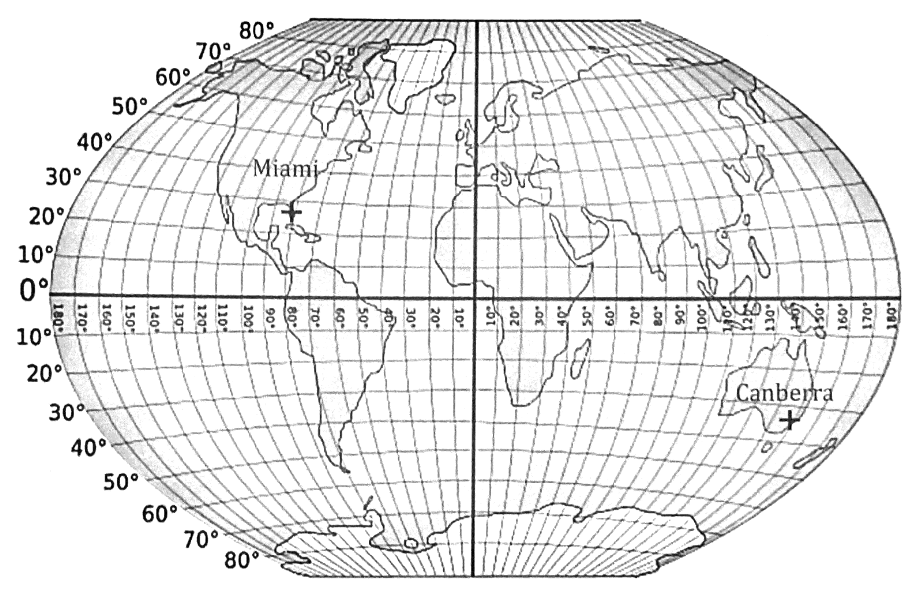
\includegraphics{planisphere.eps}};
		\draw
			(0:1) node[right]{E} --
			(45:0.2) --
			(90:1) node[above]{N} --
			(135:0.2)--
			(180:1) node[left]{O} --
			(215:0.2) --
			(-90:1) node[below]{S} --
			(-45:0.2) -- cycle;
			\foreach \a in {0,90,180,270}
				\fill[fill=black] (0,0)--(\a:1)--(\a+45:.2)--cycle;

	\end{tikzpicture}

\end{center}

On représente la Terre, l'ISS et son orbite (trajectoire de l’ISS) à l'aide du schéma ci-dessous.

\medskip

\begin{minipage}{8cm}
	On considère que:
\begin{itemize}
	\item la Terre est assimilée a une sphère de rayon \np[km]{6371};

	\item l’orbite de l’ISS est un cercle de même centre que celui de la Terre ;

	\item l’ISS tourne autour de la Terre a une altitude de $380$ km.
\end{itemize}
\end{minipage}
\hfill
\begin{tikzpicture}[baseline={(0,0)}]
	\draw[draw = gray,fill=gray!30] (0,0) circle (1.8);
	\draw (-0.2,0)--(0.2,0) (0,-0.2)--(0,0.2);
	\draw[line width=1 pt, dashed] (0,0) circle (3);
	\draw [line width = 1pt , <->,> = stealth]
		(0,0)--(-32:1.8) node [pos=.5,below,sloped] {\np[km]{6371}}
		(56:1.8)--(56:3) node [pos=.5,below,sloped] {\np[km]{380}};

		\fill[line width=0.8pt,fill=black,shift={(0,0)}] (-3.515,0.382) -- (-3.399,0.430) -- (-3.263,-0.069) -- (-3.350,-0.115) -- cycle;
		\fill[line width=0.8pt,fill=black,shift={(0,0)}] (-3.348,0.452) -- (-3.243,0.495) -- (-3.144,-0.006) -- (-3.224,-0.048) -- cycle;
		\fill[line width=0.8pt,fill=black,shift={(0,0)}] (-2.745,0.703) -- (-2.666,0.736) -- (-2.689,0.234) -- (-2.753,0.200) -- cycle;
		\fill[line width=0.8pt,fill=black,shift={(0,0)}] (-2.622,0.754) -- (-2.546,0.785) -- (-2.592,0.285) -- (-2.654,0.252) -- cycle;
		\fill[line width=0.8pt,fill=black,shift={(0,0)}] (-3.427,0.116) -- (-3.020,0.309) -- (-3.011,0.325) -- (-3.003,0.434) -- (-2.932,0.395) -- (-2.927,0.358) -- (-2.570,0.522) -- (-2.573,0.497) -- (-2.804,0.386) -- (-2.810,0.215) -- (-2.862,0.215) -- (-2.875,0.352) -- (-2.937,0.323) -- (-2.937,0.224) -- (-2.930,0.164) -- (-2.929,0.106) -- (-2.901,0.082) -- (-2.948,0.042) -- (-2.990,0.068) -- (-2.973,0.083) -- (-2.974,0.204) -- (-2.990,0.207) -- (-3.029,0.214) -- (-3.032,0.106) -- (-3.086,0.108) -- (-3.091,0.248) -- (-3.418,0.091) -- cycle;
\end{tikzpicture}

\begin{enumerate}[resume]
	\item Montrer que l’ISS parcourt environ \np[km]{42400} pour effectuer un tour complet de la Terre.

	\item On estime que l’ISS tourne autour de la Terre à la vitesse moyenne de \np[km/h]{27600}.
	\begin{enumerate}
		\item Montrer qu’il faut environ 1~h~32~min à l'ISS pour effectuer un tour complet de la Terre.
		\item Le 19 juin 2020, de 14~h~30 à 21~h~45 (heure de Paris), le spationaute français Thomas Pesquet a effectué une sortie extravéhiculaire en restant attaché à |’ISS.

		Durant cette sortie, combien de fois Thomas Pesquet a-t-il fait le tour complet de la Terre ?
	\end{enumerate}
\end{enumerate}
%%%%  fin Asie 20 juin 2022
\newpage
%%%%%%%%%%%%%  Polynésie 20 juin 2022
\hypertarget{Polynesie}{}

\label{Polynesie}

\lfoot{\small{Polynésie}}
\rfoot{\small{23 juin 2022}}
\marginpar{\rotatebox{90}{\textbf{A. P{}. M. E. P{}.}}}
\pagestyle{fancy}
\thispagestyle{empty}
\begin{center}

{\Large \textbf{\decofourleft~Brevet des collèges Polynésie 23 juin 2022~\decofourright}}

\bigskip

\textbf{Durée : 2 heures} \end{center}

\bigskip

\textbf{Exercice 1 \hfill 20 points}

\medskip

Pour chacune des quatre affirmations suivantes, dire si elle vraie ou fausse en expliquant soigneusement la réponse.

\medskip

\begin{enumerate}
\item Adriana doit effectuer le calcul suivant :

\[- \dfrac75 + \dfrac65 \times \dfrac47\]\index{calcul de fractions}


\textbf{Affirmation 1 :} Le résultat qu'elle obtient sous forme de fraction irréductible est $- \dfrac{4}{35}$.
\item Sur la figure ci-dessous, qui n'est pas à l'échelle, les points G, A et R sont alignés et les points E, A et M sont alignés.\index{Thalès}

\begin{center}
\psset{unit=1cm}
\begin{pspicture}(11.5,5)
%\psgrid
\psline(0,5)(5.5,0)%GE
\psline(6,5)(11.5,0)%MR
\psline(0.5,4.58)(10.7,0.7)%GR
\psline(3.5,1.8)(8.58,2.7)%EM
\uput[l](0.4,4.6){G} \uput[u](6.43,2.37){A} \uput[ur](8.58,2.7){M}
\uput[dl](3.5,1.8){E} \uput[ur](10.7,0.7){R}
\uput[u](3.8,3.35){9,8 cm} \uput[u](7.4,2.6){3 cm}
\uput[d](5.2,2.1){4,2 cm}\uput[d](8.5,1.5){7 cm}
\end{pspicture}
\end{center}

\textbf{Affirmation 2 :} Les droites (GE) et (MR) sont parallèles.\index{droites parallèles}
\item \textbf{Affirmation 3 :} La décomposition en produit de facteurs premiers de $126$ est $2 \times 7 \times 9$.\index{produit de facteurs premiers}

\item Dans la recette de sauce de salade de Thomas, les volumes de moutarde, de vinaigre et d'huile sont dans le ratio de 1 : 3 : 7.\index{ratio}

\smallskip

\textbf{Affirmation 4 :} Pour obtenir $330$ mL de sauce de salade, il faut utiliser $210$ mL d'huile
\end{enumerate}

\bigskip

\textbf{Exercice 2 \hfill 16 points}

\medskip

Le graphique ci-dessous représente les deux tarifs pratiqués dans une salle de sport, selon le nombre d'heures effectuées :

\setlength\parindent{9mm}
\begin{itemize}
\item[$\bullet~~$] la droite $\left(d_1\right)$ est la représentation graphique du tarif \og liberté \fg
\item[$\bullet~~$]la droite $\left(d_2\right)$ est la représentation graphique du tarif \og abonné \fg
\end{itemize}
\setlength\parindent{0mm}\index{fonction linéaire}\index{fonction linéaire}

%%%%%%
\begin{center}
\psset{xunit=1cm,yunit=0.2cm}
\begin{pspicture}(-1,-4)(11,35)
\multido{\n=0+1}{12}{\psline[linewidth=0.4pt](\n,0)(\n,35)}
\multido{\n=0+5}{8}{\psline[linewidth=0.4pt](0,\n)(11,\n)}
\psaxes[linewidth=1.25pt,Dy=5,labelFontSize=\scriptstyle]{->}(0,0)(0,0)(11,35)
\psplot[plotpoints=400,linewidth=1.25pt,linecolor=red]{0}{11}{2.5 x mul 7.5 add}
\psplot[plotpoints=400,linewidth=1.25pt,linecolor=blue]{0}{7}{5 x mul}
\uput[u](6.5,33){\blue $\left(d_1\right)$}
\uput[u](10.3,33){\red $\left(d_2\right)$}
\rput{90}(-1,26){Prix payé en euro}
\uput[d](9,-2){Nombres d'heures effectuées}
\end{pspicture}
\end{center}

\begin{enumerate}
\item Le prix payé avec le tarif \og liberté \fg{} est-il proportionnel au nombre d'heures effectuées dans la salle de sport ? Expliquer la réponse.
\item On appelle:

\setlength\parindent{9mm}
\begin{itemize}
\item[$\bullet~~$]$f$ la fonction qui, au nombre d'heures effectuées, associe le prix payé en euro avec le tarif \og liberté \fg
\item[$\bullet~~$]$g$ la fonction qui, au nombre d'heures effectuées, associe le prix payé en euro avec le tarif \og abonné \fg
\end{itemize}
\setlength\parindent{0mm}

Répondre aux questions suivantes par lecture graphique :
	\begin{enumerate}
		\item Quelle est l'image de 5 par la fonction $f$ ?\index{image}
		\item Quel est l'antécédent de 10 par la fonction $g$ ?\index{antécédent}
	\end{enumerate}
\item À l'aide du graphique, indiquer le tarif parmi les deux proposés qui est le plus avantageux pour une personne selon le nombre d'heures qu'elle souhaite effectuer dans la salle de sport.
\item Déterminer le prix payé avec le tarif \og liberté \fg{} pour $15$ heures effectuées.\index{lecture graphique}

Expliquer la démarche, même si elle n'est pas aboutie.
\end{enumerate}

\bigskip

\textbf{Exercice 3 \hfill 23 points}

\medskip

\emph{Les deux parties de cet exercice sont indépendantes}

\medskip

Une entreprise produit et vend des jus de fruit contenus dans des briques en carton qui ont la forme d'un pavé droit.

\bigskip

\textbf{PARTIE A : Briques de jus de pomme}

\medskip

Ces briques sont fabriquées pour contenir 350 mL de jus de pomme.

\smallskip

Lors d'un contrôle, 24 briques sont prélevées au hasard et analysées.

Le tableau ci-dessous donne le volume de jus de pomme (en mL) contenu dans ces briques :

\begin{center}
\begin{tabularx}{\linewidth}{|m{2.5cm}|*{11}{>{\centering \arraybackslash}X|}}\hline
Volume en mL&344 &347 &348 &349 &350 &351& 352 &353 &354 &356 &357\\ \hline
Effectif &1&2 &4 &4 &2 &3 &1&2 &3 &1 &1\\ \hline
\end{tabularx}
\end{center}

\medskip

\begin{enumerate}
\item Déterminer la médiane des volumes de cette série. Interpréter ce résultat.\index{médiane}
\item Calculer l'étendue de cette série
\item On prélève au hasard une brique parmi celles contrôlées, quelle est la probabilité qu'elle contienne exactement $350$~mL de jus de pomme ?\index{probabilité}
\item Lorsque le volume de jus de pomme contenu dans une brique est compris entre $345$~mL et $355$~mL, cette brique peut être vendue. 

Quel est le pourcentage de briques que l'entreprise peut vendre parmi les briques contrôlées ?\index{pourcentage}
\end{enumerate}

\bigskip

\textbf{PARTIE B : Briques de jus de raisin}

\medskip

\begin{minipage}{0.67\linewidth}
L'entreprise souhaite commercialiser une nouvelle brique en forme de pavé droit pour le jus de raisin. Sa base est un rectangle de longueur $6,4$ cm et de largeur $5$ cm.

\medskip

\begin{enumerate}
\item Calculer l'aire de la base de cette brique
\item Quelle doit être la hauteur de cette brique pour que son volume soit de $400$~cm$^3$ ?
\end{enumerate}
\end{minipage}\hfill
\begin{minipage}{0.28\linewidth}
\psset{unit=1cm}
\begin{pspicture}(3.4,4.5)
%\psgrid
\pspolygon(0,3.8)(0,0.8)(2,0.1)(2,3.1)
\psline(2,0.1)(3.4,0.7)(3.4,3.7)(2,3.1)
\psline(3.4,3.7)(1.4,4.4)(0,3.8)
\psline[linestyle=dashed](0,0.8)(1.4,1.4)(3.4,0.7)
\psline[linestyle=dashed](1.4,1.4)(1.4,4.4)
\uput[d](1,0.42){6,4 cm}\uput[d](2.7,0.35){5 cm}
\end{pspicture}
\end{minipage}

\bigskip

\textbf{Exercice 4 \hfill 20 points}

\medskip

On considère le programme de calcul suivant :\index{programme de calcul}

\begin{center}
\psset{unit=0.75cm,arrowsize=2pt 3}
\begin{pspicture}(-5,0)(5,11)
%\psgrid
\rput(0,10.8){Choisir un nombre}
\psline{->}(0,10.7)(0,10)
\psframe(-1.5,9)(1.5,10)
\rput(-3,8.5){Ajouter 5}
\psline{->}(0,9)(-3,7.6)\psline{->}(0,9)(3,7.6)
\psframe(-4,6.6)(-2,7.6)\psframe(4,6.6)(2,7.6)
\rput(3,8.5){Soustraire 5}
\psline{->}(-3,6.6)(0,4)(0,3)\psline(3,6.6)(0,4)
\rput(0,5.8){Multiplier les deux}
\rput(0,5.4){résultats}
\psframe(-1,3)(1,2)
\psline{->}(0,2)(0,1)
\rput(1.3,1.6){Ajouter 25}
\psframe(-1,1)(1,0)
\end{pspicture}
\end{center}

%\medskip

\begin{enumerate}
\item 
	\begin{enumerate}
		\item Si on choisit le nombre $7$, vérifier qu'on obtient 49 à la fin du programme
		\item Si on choisit le nombre $- 4$, quel résultat obtient-on à la fin du programme ?
	\end{enumerate}	
\item On note $x$ le nombre choisi au départ
	\begin{enumerate}
		\item Exprimer en fonction de $x$ le résultat obtenu.
		\item Développer et réduire $(x + 5)(x - 5)$.\index{développement}
		\item Sarah dit : \og Avec ce programme de calcul, quel que soit le nombre choisi au départ, le résultat obtenu est toujours le carré du nombre de départ \fg.
		
Qu'en pensez-vous ?
	\end{enumerate}
\end{enumerate}

\bigskip

\textbf{Exercice 5 \hfill 23 points}

\medskip

\begin{minipage}{0.42\linewidth}
Le centre Pompidou est un musée d'art contemporain à Paris. Pour accéder aux étages, il faut utiliser un ensemble d'escalators extérieurs appelé \og chenille \fg.

La chenille est composée de 5 escalators tous identiques (traits épais sur la figure ci-dessous) et de 6 passerelles horizontales toutes identiques (traits fins horizontaux sur la figure ci-dessous).
\end{minipage}\hfill
\begin{minipage}{0.56\linewidth}
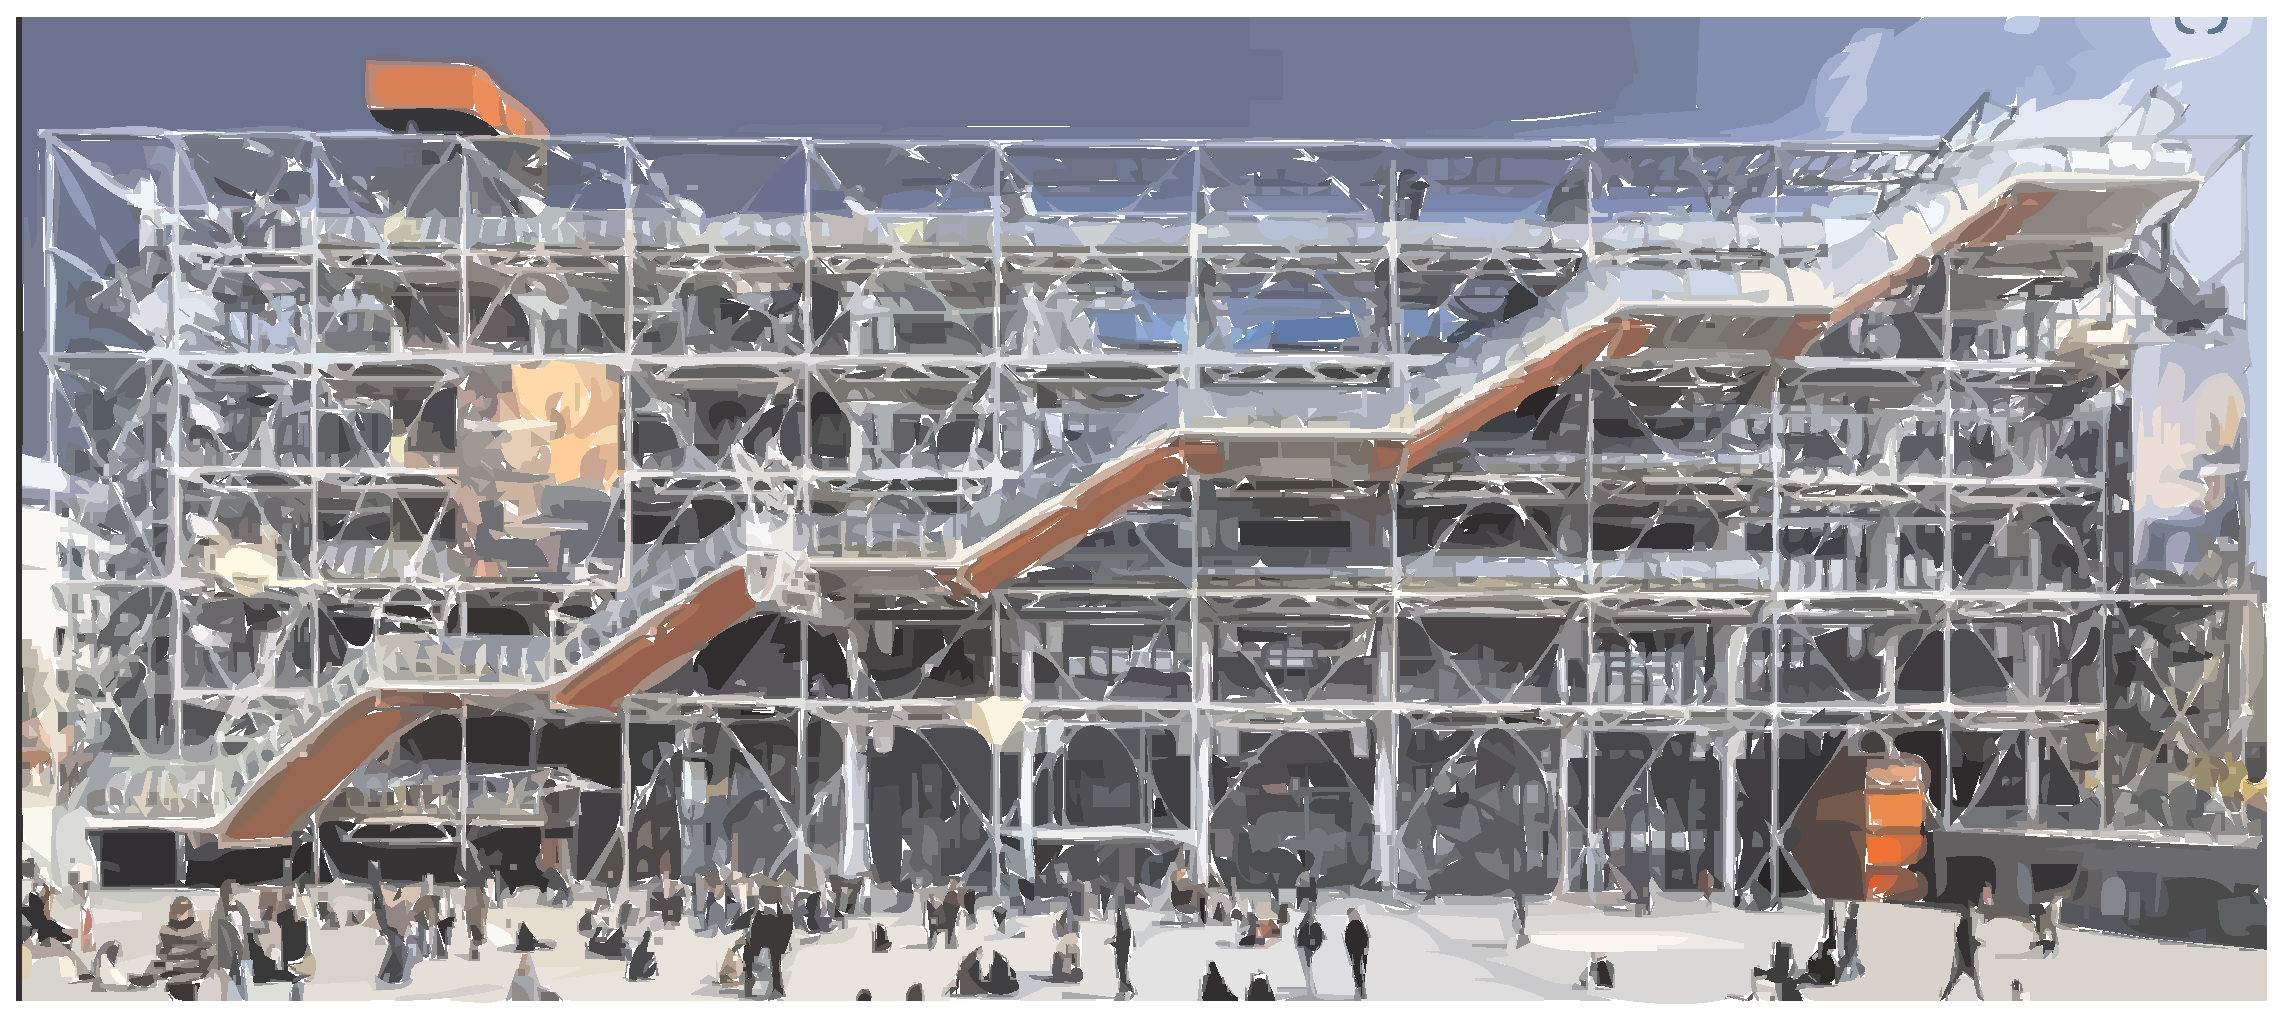
\includegraphics[width=8cm]{Pomp}
\end{minipage}

\begin{center}
\psset{unit=1cm,arrowsize=2pt 3}
\begin{pspicture}(13.5,4.6)
%\psgrid
\psline{<->}(0,0.2)(12.1,0.2)\uput[d](6.05,0.2){135 m}
\psline{<->}(12.7,0.6)(12.7,3.6)\uput[r](12.7,2.25){32 m}
\def\esca{\psline[linewidth=0.5pt](0,0)(1.1,0)\psline[linewidth=0.2pt](0.5,-0.1)(0.5,0.1)\psline[linewidth=0.2pt](0.6,-0.1)(0.6,0.1)\psline[linewidth=1.25pt](1.1,0)(2.2,0.6)\psline[linewidth=1.25pt](1.65,0.35)(1.75,0.25)}
\multido{\n=0.0+2.2,\na=0.6+0.6}{5}{\rput(\n,\na){\esca}}
\psline[linewidth=0.2pt](11,3.6)(12.1,3.6)
\psline{<->}(11,4)(12.1,4)\uput[u](11.55,4){12,5 m}
\psline[linewidth=1.5pt,linestyle=dotted](5.5,1.8)(6.6,1.8)(6.6,2.4)\uput[d](6.05,1.8){$p$}
\uput[r](6.6,2.1){$h$}
\psline[linewidth=0.2pt](11.5,3.7)(11.5,3.5)\psline[linewidth=0.2pt](11.6,3.7)(11.6,3.5)
\psline[linewidth=1.5pt,linestyle=dotted](1.1,0.6)(12.7,0.6)
\end{pspicture}
\end{center}

\medskip

\begin{enumerate}
\item À l'aide de la figure ci-dessus :
	\begin{enumerate}
		\item Vérifier que la profondeur $p$ de chaque escalator est égale à $12$ m
		\item Calculer la hauteur $h$ de chaque escalator
	\end{enumerate}	
\end{enumerate}
\begin{minipage}{0.62\linewidth}
\begin{enumerate}[resume]
\item À l'aide du triangle RST ci-contre :
	\begin{enumerate}
		\item Prouver que la longueur ST d'un escalator est de $13,6$ m.
		\item Montrer que la mesure de l'angle formé par l'escalator avec l'horizontale (c'est-à-dire l'angle $\widehat{\text{RST}}$ arrondie au degré est de $28\degres$.\index{calcul d'angle}
	\end{enumerate}
\end{enumerate}
\end{minipage}\hfill
\begin{minipage}{0.36\linewidth}
\psset{unit=1cm}
\begin{pspicture}(4.8,2.4)
\psline[linewidth=1.5pt,linestyle=dotted](0.2,0.2)(3.8,0.2)(3.8,1.8)%SRT
\psline[linewidth=1.5pt](0.2,0.2)(3.8,1.8)
\uput[dr](3.8,0.2){R} \uput[dl](0.2,0.2){S} \uput[ur](3.8,1.8){T} \uput[d](2,0.2){12 m} \uput[r](3.8,1){6,4 m}
\end{pspicture}
\end{minipage}

\begin{enumerate}[resume*,start=3]		
\item Sabine veut représenter la chenille grâce au logiciel Scratch.

Elle a écrit le programme qui est donné sur l'ANNEXE. On précise que : 1 pas du logiciel correspond à 1 m dans la réalité.

Compléter les lignes 6, 7, 9, et 10, sur l'ANNEXE (à rendre avec la copie), afin d'obtenir le tracé ci-dessous de la chenille :\index{scratch}

\begin{center}
\psset{unit=0.8cm,arrowsize=2pt 3}
\begin{pspicture}(13.5,4.6)
\def\esca2{\psline[linewidth=0.5pt](0,0)(1.1,0)\psline[linewidth=1.25pt](1.1,0)(2.2,0.6)}
\multido{\n=0.0+2.2,\na=0.6+0.6}{5}{\rput(\n,\na){\esca2}}
\psline[linewidth=0.2pt](11,3.6)(12.1,3.6)
\end{pspicture}
\end{center}

Rappel : \og S'orienter à 90 \fg{} signifie que l'on est orienté vers la droite
\end{enumerate}

\newpage

\begin{center}

\textbf{\Large ANNEXE}

\bigskip

\textbf{\large À compléter et à rendre avec la copie}

\end{center}

\bigskip

\textbf{Exercice 5 question 3 :}

\bigskip

\begin{center}
\begin{scratch}[scale=1.75, num blocks]
\blockinit{quand \greenflag est cliqué}
\blockpen{effacer tout}
\blockmove{s'orienter à \ovalnum{90}}
\blockmove{aller à x: \ovalnum{-120} y: \ovalnum{-60}}
\blockpen{stylo en position d'écriture}
\blockrepeat{répéter \ovalnum{} fois}
{
\blockmove{avancer de \ovalnum{}}
\blockmove{tourner \turnleft{} de \ovalnum{28} degrés}
\blockmove{avancer de \ovalnum{}}
\blockmove{tourner \turnright{} de \ovalnum{} degrés}
}
\blockmove{avancer de \ovalnum{12,5}}
\blockpen{relever le stylo}
\end{scratch}
\end{center}
%%%%%%%%%%%%%  fin Polynésie 20 juin 2022
\newpage
%%%%%%%%%%%%%  Métropole 30 juin 2022
\hypertarget{Metropole}{}

\label{Metropole}

\rfoot{\small Métropole Antilles-Guyane}
\lfoot{\small 30 juin 2022}
\pagestyle{fancy}
\thispagestyle{empty}
\begin{center}
{\Large\textbf{\decofourleft~ Diplôme national du Brevet
 ~\decofourright}}\\[6pt]
{\Large \textbf{Métropole  Antilles-Guyane\hspace{1.5em}30 juin 2022}}

\vspace{0,5cm}

\textbf{Durée : 2 heures}
\end{center}
\medskip

\emph{L'usage de calculatrice avec mode examen activé est autorisé.\\
L'usage de calculatrice sans mémoire \og type collège \fg{} est autorisé\\
L'utilisation du dictionnaire est interdite.}

\vspace{0,5cm}
\framebox[16cm]{
\begin{minipage}{15cm}
\begin{center}
\textbf{Indications portant sur l'ensemble du sujet.}
\end{center}
 Toutes les réponses doivent être justifiées, sauf si une indication contraire est donnée.\\
Pour chaque question, si le travail n’est pas terminé, laisser tout de même une trace de la 
recherche ; elle sera prise en compte dans la notation.
\end{minipage}
}
\vspace{0.75cm}

\textbf{{\large \textsc{Exercice 1}} \hfill 20 points}


Une famille se promène au bord d’une rivière.

Les enfants aimeraient connaître la largeur de la rivière.

Ils prennent des repères, comptent leurs pas et dessinent le schéma ci-dessous sur lequel les points C, E et D, de même que A, E et B sont alignés. (Le schéma n'est pas à l’échelle.)

\begin{center}
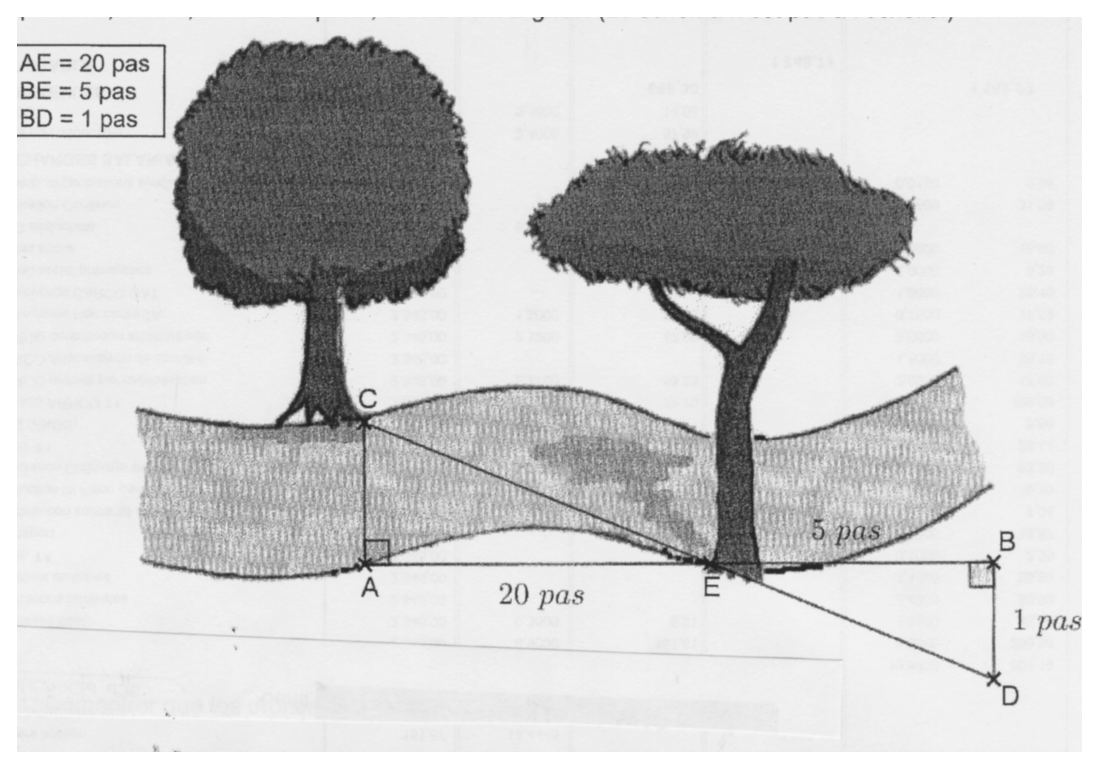
\includegraphics[scale=0.5]{riviere-2}
\end{center}

\begin{enumerate}
\item Démontrer que les droites (AC) et (BD) sont parallèles.\index{droites parallèles}
\item Déterminer, en nombre de pas, la largeur AC de la rivière.\index{Thalès}
\end{enumerate}

 Pour les questions qui suivent, on assimile la longueur d'un pas à 65~cm.

\medskip

\begin{enumerate}[resume]
\item Montrer que la longueur CE vaut $13,3$~m, en arrondissant au décimètre près.
\item 
	\begin{enumerate}
		\item  L’un des enfants lâche un bâton dans la rivière au niveau du point E. Avec le courant, le bâton se déplace en ligne droite en 5 secondes jusqu'au point C.

Calculer la vitesse du bâton en m/s.
	\item Est-il vrai que \og le bâton se déplace à une vitesse moyenne inférieure à \np[km/h]{10}\fg?\index{moyenne}
	\end{enumerate}
\end{enumerate}

\bigskip

\textbf{{\large \textsc{Exercice 2}} \hfill 20 points}

\medskip 
Cet exercice est un questionnaire à choix multiples (QCM). Aucune justification n'est demandée.\index{QCM}

Pour chaque question, trois réponses (A, B et C) sont proposées. \textbf{Une seule réponse est exacte.}

Recopier sur la copie le numéro de la question et la réponse.

\medskip
 
{\footnotesize
\begin{tabularx}{\linewidth}{|m{8cm}|*{3}{>{\centering \arraybackslash}X|}}\hline
\centering{Questions} & Réponse A & Réponse B & Réponse C \\
\hline
\begin{minipage}{7.5cm}
\textbf{1.} On considère les deux figures suivantes.

Par quelle transformation la figure 2 est-elle l'image de la figure 1 ?

\psset{xunit=1.cm,yunit=1.cm,labelFontSize=\scriptstyle}
\begin{pspicture}(-1,-0.5)(5,3.5)
\pscustom[fillcolor=lightgray,fillstyle=solid]{\psline(0,2)(0,3)\psline(0,3)(1,3)\psline(1,3)(1,2)\psline(1,2)(2,1)\psline(2,1)(1,1)\psline(1,1)(0,2)}
\pscustom[fillstyle=solid,fillcolor=lightgray]{\psline(3,1)(3,2)\psline(3,2)(4,2)\psline(4,2)(4,1)\psline(4,1)(5,0)\psline(5,0)(4,0)\psline(4,0)(3,1)}
\multido{\n=0+1}{6}{\psline[linewidth=0.75pt,linecolor=gray](\n,-0.4)(\n,3.2)}
\multido{\n=0+1}{4}{\psline[linewidth=0.75pt,linecolor=gray](-0.2,\n)(5,\n)} 
\uput[ur](1,3){B}\uput[ur](1,2){A}\uput[dr](1,1){E}
\uput[ur](4,2){B'}\uput[ur](4,1){A'}\uput[dr](4,0){E'}
\psline[linewidth=0.15pt,linecolor=lightgray]{->}(1,3)(4,2)
\psline[linewidth=0.15pt,linecolor=lightgray]{->}(1,2)(4,1)
\psline[linewidth=0.15pt,linecolor=lightgray]{->}(1,1)(4,0)
\uput[u](0.5,2){\huge\ding{192}} \uput[u](3.5,1){\huge\ding{193}}
\end{pspicture}
\end{minipage}
&une translation & une homothétie & une symétrie axiale\\\hline\index{translation}\index{homothétie}\index{symétrie axiale}
\begin{minipage}{5cm}
\textbf{2.} On considère la représentation graphique de la fonction $g$ suivante :

\psset{unit=0.8cm,labelFontSize=\scriptstyle}
\begin{pspicture}(-3,-1)(4,5.2)
\multido{\n=-1+1}{6}{\psline[linewidth=0.75pt,linecolor=lightgray](\n,-1)(\n,5.1)}
\multido{\n=-1+1}{7}{\psline[linewidth=0.75pt,linecolor=lightgray](-1.1,\n)(4.1,\n) }
\psaxes[linewidth=0.95pt]{->}(0,0)(-1.1,-1.1)(4.1,5.1)
\psplot[linewidth=1.5pt,linecolor=blue,plotpoints=5000]{-0.50}{2.5}{x 2  mul }
\end{pspicture}

Quel est l'antécédent de 2 par la fonction $g$.\index{antécédent}
\end{minipage}
&2&1&4\\\hline 

\begin{minipage}{7.5cm}

\smallskip
\textbf{3.} Soit $f$ la fonction définie par :
\[f(x)= 3x^2-7 \]
Quelle affirmation est correcte ? 
\end{minipage}
&
 29 est l'image de 2 par la fonction $f$& $f(3) = 20$&$f$ est une fonction affine.\\
\hline\index{fonction affine}

\begin{minipage}{7.5cm}
\smallskip
\textbf{4.} On a relevé les performances, en mètres, obtenues au lancer du poids
 par un groupe de 13 élèves d'une classe.
\np[m]{3,41} ; \np[m]{5.25} ; \np[m]{5.42} ; \np[m]{4.3} ; \np[m]{6.11} ;
\np[m]{4.28} ; \np[m]{5,15} ; \np[m]{3,7} ; \np[m]{6,07} ;
\np[m]{5,82} ; \np[m]{4,62} ; \np[m]{4,91} ; \np[m]{4,01}

Quelle est la médiane de cette série de valeurs ?
\end{minipage}
& 7&\np{4.91}&\np{5.15}\\
\hline
%\end{tabularx}
\begin{minipage}{7.5cm}

\smallskip
\textbf{5.} On considère la configuration suivante, dans laquelle les
triangles LAC et BUT sont semblables. 

\psset{xunit=0.5cm,yunit=0.5cm,linewidth=0.5pt}
\begin{pspicture}(-1.5,-0.5)(7,6.75)
\psline(0,3)(2.49,2.84)\psline(0,3)(1.1,4.79)\psline(1.1,4.79)(2.49,2.84)
\psline(3.7,0)(6.99,5.37)\psline(3.7,0)(11.18,-0.48)\psline(11.18,-0.48)(6.99,5.37)
\uput[l](0,3){L}\uput[u](1.1,4.79){A}\uput[r](2.5,2.9){C}
\uput[l](3.7,0){B}\uput[u](6.99,5.37){U}\uput[r](11.18,-0.48){T}
\labelsep=1pt
\uput[l](0.5,3.7){\np[cm]{2.1}}\uput[dl](2,2.5){\np[cm]{2.5}}\uput[ur](2,3.5){\np[cm]{2.4}}
\uput[dr](3.8,2.7){\np[cm]{6.3}}\uput[dl](6.5,-0.45){\np[cm]{7.5}}\uput[ur](8.6,3.1){\np[cm]{7.2}}
\end{pspicture}

\medskip
Par quel nombre doit-on multiplier l'aire du triangle LAC pour obtenir l'aire du triangle BUT ?\index{aire}
\end{minipage}
&3&6&9\\\hline
\end{tabularx}
}
\bigskip

\textbf{{\large \textsc{Exercice 3}} \hfill 20 points}

\medskip

Une collectionneuse compte ses cartes Pokémon afin de les revendre. Elle possède 252 cartes de type \og feu \fg{} et 156 cartes de type \og terre \fg.
\begin{enumerate}
\item  \begin{enumerate}
\item  Parmi les trois propositions suivantes, laquelle correspond à la décomposition en produit de facteurs premiers du nombre 252 :

\begin{center}
\begin{tabularx}{9cm}{|*{3}{>{\centering \arraybackslash}X|}}\hline
Proposition 1 &Proposition 2& Proposition 3\\
 $2^2\times 9\times 7$ &$2\times 2\times 3\times 21$ &$2^2 \times 3^2\times  7$\\\hline
\end{tabularx}
\end{center}
\item Donner la décomposition en produit de facteurs premiers du nombre $156$.\index{produit de facteurs premiers}
\end{enumerate}
\item Elle veut réaliser des paquets identiques, c'est-à-dire contenant chacun le même nombre de cartes \og terre \fg{} et le même nombre de cartes \og feu \fg{} en utilisant toutes ses cartes.
\begin{enumerate}
\item Peut-elle faire 36 paquets ?
\item Quel est le nombre maximum de paquets qu'elle peut réaliser ?\index{pgcd}
\item Combien de cartes de chaque type contient alors chaque paquet ?
\end{enumerate}
\item Elle choisit une carte au hasard parmi toutes ses cartes. On suppose les cartes  indiscernables au toucher.

Calculer la probabilité que ce soit une carte de type \og terre \fg.\index{probabilité}
\end{enumerate}

\vspace{0.5cm}

\textbf{{\large \textsc{Exercice 4}} \hfill 20 points}

\medskip

Dans cet exercice, $x$ est un nombre strictement supérieur à 3.

On s'intéresse aux deux figures géométriques dessinées ci-dessous :
\begin{itemize}
\item un rectangle dont les côtés ont pour longueurs $x-3$ et $x+7$.
\item un carré de côté $x$.
\end{itemize}

\begin{center}
\begin{pspicture}(-1,-0.5)(13,4.5)
\psframe(0,0)(5,2)\psframe(7,0)(11,4)
\uput[l](0,1){$x - 3$}\uput[d](2.5,0){$x + 7$}\uput[l](7,2){$x$}\uput[d](9,0){$x$}
\end{pspicture}
\end{center}

\begin{enumerate}
\item Quatre propositions sont écrites ci-dessous :

Recopier sur la copie celle qui correspond à l'aire du carré. On ne demande pas de justifier.

\begin{tabularx}{\linewidth}{|*{4}{>{\centering \arraybackslash}X|}}\hline
$4x$&$4+x$&$x^2$&$2x$\\\hline
\end{tabularx}

\item  Montrer que l'aire du rectangle est égale à $x^2 + 4x - 21$.

\item On a écrit le script ci-dessous dans Scratch.\index{scratch}

On veut que ce programme renvoie l'aire du rectangle lorsque l'utilisateur a rentré une valeur de $x$ (strictement supérieure à 3).

Écrire sur la copie les contenus des trois cases vides des lignes 5, 6 et 7, en précisant les numéros de lignes qui correspondent à vos réponses.

\hspace*{2cm}
\begin{scratch}[num blocks]
\blockinit{Quand la touche\selectmenu{espace} est pressée}
\blocklook{demander \ovalnum {combien vaut x ?} et attendre}
\blockvariable{mettre \selectmenu{x} à \ovalsensing{réponse}}
\blockvariable{mettre \selectmenu{R} à \ovalvariable{x}*\ovalvariable{x}}
\blockvariable{ajouter \ovalnum{}*\ovalvariable{x} à \ovalvariable{R}}
\blockvariable{ajouter \ovalnum{} à \ovalvariable{R}}
\blocklook{dire \ovaloperator{regrouper \ovalnum{L'aire du rectangle est }et \ovalnum{}} pendant \ovalnum{2} secondes}
\end{scratch}\\

\item On a pressé la touche espace puis saisi le nombre 8. Que renvoie le programme ?

\item Quel nombre $x$ doit-on choisir pour que l'aire du rectangle soit égale à l'aire du carré ?

\emph{Toute trace de recherche, même non aboutie, sera prise en compte.} 
\end{enumerate}


\vspace{0.5cm}

\textbf{{\large \textsc{Exercice 5}} \hfill 20 points}

\medskip

Dans une habitation, la consommation d'eau peut être anormalement élevée lorsqu’il y a une fuite d'eau.

On considère la situation suivante :
\begin{itemize}
\item Une salle de bain est équipée d'une vasque de forme cylindrique, comme l'illustre l'image ci-dessous.

\item Le robinet fuit à raison d'une goutte par seconde.

\item En moyenne, 20 gouttes d'eau correspondent à un millilitre (\np[ml]{1} ).
\end{itemize}

\begin{multicols}{2}
\begin{minipage}[7cm]{8cm}
\phantom{x}
\includegraphics[scale=0.5]{vasque.ps}
\end{minipage}

\columnbreak

~\\\\\\

\begin{tabular}{|l|}\hline

Caractéristiques de la vasque :\\

\hspace{2em}Diamètre intérieur : \np[cm]{40}\\

\hspace{2em}Hauteur intérieure : \np[cm]{15} \\

\hspace{2em}Masse : \np[kg]{25} \\\hline
\end{tabular}
\end{multicols}
\medskip

Rappels : \hspace{4em} \begin{tabular}{|c|}\hline

Volume du cylindre = $\pi \times \text{rayon}^2 \times \text{hauteur}$\\

\hspace{2.5em} \np[dm^3]{1} = 1 litre\\
\hline
\end{tabular}

\begin{enumerate}
\item En raison de la fuite, montrer qu'il tombe \np{86400}~gouttes dans la vasque en une journée complète.

\item Calculer, en litres, le volume d'eau qui tombe dans la vasque en une semaine en raison de la fuite.

\item  Montrer que la vasque  a un volume de \np{18.85}~litres, arrondi au centilitre près.\index{volume}

\item L'évacuation de la vasque est fermée et le logement inoccupé pendant une semaine. L'eau va-t-elle déborder de la vasque ? Justifier la réponse.
\item  À la fin du XIX\ieme{} siècle, la consommation domestique d'eau par habitant en France était d'environ 17 litres par jour. Elle a fortement augmenté avec la généralisation de la distribution d'eau par le robinet dans les domiciles : elle est passée à $165$~litres par jour et par habitant en 2004.

En 2018, la consommation des Français baisse légèrement pour atteindre $148$~litres d'eau par jour et par habitant.

Calculer le pourcentage de diminution de la consommation quotidienne d'eau par habitant entre 2004 et 2018. On arrondira ce pourcentage à l'unité.
\end{enumerate}
%%%%%%%%%%%%%  fin Métropole 30 juin 2022
\newpage
%%%%%%%%%%%%%  Métropole 30 juin 2022 sujet de secours
\hypertarget{Metropole_secours}{}

\label{Metropole_secours}

\rfoot{\small Métropole Antilles-Guyane (secours)}
\lfoot{\small 30 juin 2022}
\pagestyle{fancy}
\thispagestyle{empty}
\begin{center}
{\Large\textbf{\decofourleft~ Diplôme national du Brevet
 ~\decofourright}}\\[6pt]
{\Large \textbf{Métropole  Antilles-Guyane\hspace{1.5em}Sujet de secours 30 juin 2022}}

\vspace{0,5cm}

\textbf{Durée : 2 heures}
\end{center}
\medskip

\vspace{0,5cm}
\framebox[16cm]{
\begin{minipage}{15cm}
\begin{center}
\textbf{Indications portant sur l'ensemble du sujet.}
\end{center}
Toutes les réponses doivent être justifiées, sauf si une indication contraire est donnée.\\
Pour chaque question, si le travail n’est pas terminé, laisser tout de même une trace de la 
recherche ; elle sera prise en compte dans la notation.
\end{minipage}
}
\vspace{0.75cm}

\textbf{{\large \textsc{Exercice 1}} \hfill 20 points}

\medskip

Voici cinq affirmations. Pour chacune d'entre elles, dire si elle est vraie ou fausse. Chaque réponse doit être justifiée.\index{Vrai-Faux}

\begin{minipage}{0.6\linewidth}
\begin{enumerate}
\item Lors d'une fête foraine, un stand propose de faire tourner une roue pour gagner un lot (porte-clés, ballon ou peluche). Les 8 secteurs angulaires sont de même mesure.\index{probabilité}

\textbf{Affirmation 1 :} La probabilité de l'évènement \og gagner une peluche \fg{} est égale à $\dfrac12$.
\end{enumerate}
\end{minipage}\hfill
\begin{minipage}{0.36\linewidth}
\begin{center}
\psset{unit=1cm}
\begin{pspicture}(-2.8,-2.6)(2.8,3.3)
\pscircle(0,0){2.6}
\multido{\n=0+45}{8}{\psline(2.6;\n)}
\rput(1.6;22.5){Porte-clés}
\rput(1.6;67.5){Peluche}
\rput(1.9;112.5){Porte-clés}
\rput(1.8;157.5){Ballon}
\rput(1.8;202.5){Peluche}
\rput(1.9;247.5){Porte-clés}

\rput(1.6;-22.5){Peluche}
\rput(1.6;-67.5){Peluche}
\pspolygon*(-0.15,3.3)(-0.15,2.9)(-0.2,2.9)(0,2.7)(0.2,2.9)(0.15,2.9)(0.15,3.3)
\end{pspicture}
\end{center}
\end{minipage}

\begin{enumerate}[start=2]
\item \textbf{Affirmation 2 :} Le triangle ABC ci-dessous est un triangle rectangle.\index{Pythagore}

\begin{center}
\psset{unit=1cm}
\begin{pspicture}(5.8,4.3)
\pspolygon(0.6,0.3)(5.1,0.3)(0.6,3.8)%%ACB
\uput[dl](0.6,0.3){A} \uput[ul](0.6,3.8){B} \uput[dr](5.1,0.3){C}
\uput[d](2.85,0.3){6} \uput[l](0.6,2.05){4,5} \uput[ur](2.85,2.05){7,5}
\end{pspicture}
\end{center}


\item Pour son anniversaire, Chloé invite deux de ses amis, Hakim et Manon.\index{probabilité}

Quand arrive l'heure du gâteau, les trois enfants indiquent:

$\bullet~~$Hakim : \og Je souhaite en manger les $\dfrac37$ \fg{} ;

$\bullet~~$Manon: \og Cela me fait plaisir d'en manger les $\dfrac25$ \fg{} ;

$\bullet~~$Chloé: \og $\dfrac17$ du gâteau me convient parfaitement \fg.

\textbf{Affirmation 3 :}  Les trois amis ont mangé la totalité du gâteau.

\item \textbf{Affirmation 4 :}\index{développement}

\[(2x + 3)(5x - 4) - 5(3x - 2) = 10x^2 - 8x - 2\]

\item Les angles d'un triangle DEF sont tels que :

$\bullet~~$$\widehat{\text{DFE}} = 30\degres$

$\bullet~~$La mesure de l'angle $\widehat{\text{DEF}}$ est le quadruple de celle de l'angle $\widehat{\text{FDE}}$.

\textbf{Affirmation 5 :} Le triangle DEF est un triangle isocèle.\index{calcul d'angle}
\end{enumerate}

\bigskip

\textbf{{\large \textsc{Exercice 2}} \hfill 20 points}

\medskip

L'artiste français Jean Lurçat a produit dix tapisseries de surfaces différentes, exposées dans la ville d'Angers.

La surface approximative de chacune de ces tapisseries a été saisie dans la feuille de calcul ci-dessous. (source: https://musees.angers.fr)

\begin{center}
\begin{tabularx}{0.6\linewidth}{|c|c|>{\centering \arraybackslash}X|}\hline
1&\textbf{Nom de la tapisserie}			&\textbf{Surface (en m$^2$)}\\ \hline
2&La Grande Menace				&39,2\\ \hline
3&L'homme d'Hiroshima			&12,8\\ \hline
4&Le Grand charnier				&32,4\\ \hline
5&La Fin de tout				&10,2\\ \hline
6&L'Homme en gloire dans la paix&57,5\\ \hline
7&L'eau et le feu				&27,2\\ \hline
8&Champagne						&30,9\\ \hline
9&La Conquête de l'espace		&45,9\\ \hline
10&La Poésie					&45,4\\ \hline
11&Ornamentos sagrados			&45,4\\ \hline
12&\textbf{Total}				&\\ \hline
\end{tabularx}
\end{center}

\begin{enumerate}
\item Quelle tapisserie a la surface maximale ? On ne demande pas de justifier.
\item Vérifier que la surface médiane de ces tapisseries est égale à 35,8~m$^2$.\index{médiane}
\item Quelle formule peut-on saisir dans la cellule B12 afin de calculer la surface totale de ces
dix tapisseries ?\index{tableur}

On ne demande pas de justifier.
\item Calculer la surface moyenne de ces tapisseries.\index{moyenne}
\item Sara affirme: \og 40\% de ces tapisseries ont une surface supérieure à 45 m$^2$ \fg.\index{pourcentage}

Sara a-t-elle raison ? Justifier.
\end{enumerate}

\bigskip

\textbf{{\large \textsc{Exercice 3}} \hfill 20 points}

\medskip

Un club de sport propose une nouvelle formule annuelle pour ses adhérents :

\og Achat d'une carte d'adhésion à 32~\euro{} donnant droit à un tarif de 4,50~\euro{} par séance \fg.

\medskip

\begin{enumerate}
\item Déterminer le coût à payer pour dix séances dans l'année avec cette formule.
\item Noé a un budget annuel de $95$~\euro{} pour se rendre dans cette salle de sport.

Combien de séances pourrait-il effectuer ?
\item On note $p$ la fonction qui, au nombre $x$ de séances pratiquées, associe le prix à payer pour $x$ séances pratiquées dans l'année.\index{fonction affine}
	\begin{enumerate}
		\item Donner l'expression de $p(x)$.
		\item Vérifier que $p(27) = 153,5$.\index{antécédent}\index{image}
		\item Interpréter par une phrase l'égalité précédente.
\end{enumerate}
\item On s'intéresse au programme qui permet de donner le prix à payer en fonction du nombre de séances pratiquées dans cette salle de sport.\index{scratch}

\begin{center}
\begin{scratch}[num blocks]
\blockinit{Quand \greenflag est cliqué}
\blocksensing{demander \txtbox{Choisir un nombre de séances} et attendre}
\blockvariable{mettre \ovalvariable{nombre de séances} à \ovaloperator{\ovalvariable{réponse}}}
\blockvariable{mettre \ovalvariable{résultat} à \ovaloperator{\ovalvariable{nombre de séances}*\ovalnum{\ldots \ldots}}}
\blockvariable{mettre \ovalvariable{résultat} à \ovaloperator{\ovalnum{\ldots \ldots}+\ovalvariable{resultat}}}
\blocklook{dire \ovaloperator{regrouper \txtbox{le prix à payer est} et \ovalvariable{résultat}} pendant \ovalnum{2} secondes}
\end{scratch}
\end{center}

Compléter sur l'ANNEXE  les lignes 4 et 5 pour que ce script corresponde au programme souhaité.
\end{enumerate}

\bigskip

\textbf{{\large \textsc{Exercice 4}} \hfill 18 points}

\medskip

Le Tour de France 2021 est une compétition de cyclisme s'étant déroulée du 26 juin au 18 juillet 2021.

L'étape 5 était un contre-la-montre individuel de $27,2$~km. Le graphique ci-dessous indique le temps effectué par Tadej Pogacar en fonction de la distance parcourue sur son trajet (source : https://www.letour.fr).

\medskip

On répondra aux questions suivantes à l'aide de ce graphique reproduit en annexe.

On laissera les traits de construction éventuels sur le graphique de l'annexe.

\begin{center}
\psset{xunit=0.2cm,yunit=0.15cm,arrowsize=2pt 3}
\begin{pspicture}(-5,-5)(32,43)
\psaxes[linewidth=1.25pt,labelFontSize=\scriptstyle,Dx=5,Dy=5]{->}(0,0)(0,0)(32,43)
\multido{\n=0+1}{33}{\psline[linewidth=0.1pt](\n,0)(\n,43)}
\multido{\n=0+5}{7}{\psline[linewidth=0.5pt](\n,0)(\n,43)}
\multido{\n=0+1}{44}{\psline[linewidth=0.1pt](0,\n)(32,\n)}
\multido{\n=0+5}{9}{\psline[linewidth=0.5pt](0,\n)(32,\n)}
\psline[linewidth=1.25pt,linecolor=blue](27.2,32)
\uput[u](26,0){distance (en km)}\uput[r](0,42){durée (en minutes)}
\end{pspicture}
\end{center}

\begin{enumerate}
\item Quelle distance approximative Tadej POGACAR a-t-il parcouru en 20 minutes ?\index{lecture graphique}
\item En combien de temps environ Tadej POGACAR a-t-il effectué les $27,2$ km du parcours ?
\item Le cycliste Bryan Coquard a lui aussi effectué ce contre-la-montre.

Le temps, en minutes, mis par Bryan Coquard pour parcourir la distance $x$, exprimée en km, peut être représenté par la fonction linéaire $f$ d'expression algébrique:

\[f(x) = 1,4x.\]\index{fonction linéaire}

	\begin{enumerate}
		\item Représenter la fonction $f$ sur le graphique en annexe.
		\item Lequel de ces deux coureurs a été classé avant l'autre ?
	\end{enumerate}	
\item Est-il vrai que la vitesse moyenne de Tadej Pogacar sur l'ensemble du parcours est
supérieure à $50$ km/h ? Justifier.\index{moyenne}
\end{enumerate}

\bigskip

\textbf{{\large \textsc{Exercice 5}} \hfill 22 points}

\medskip

La tour de la Vade est un monument de Carcassonne.

\begin{minipage}{0.6\linewidth}
Représentation schématique de la tour de la Vade (sans le toit).
\end{minipage}\hfill
\begin{minipage}{0.38\linewidth} 
\begin{center}
\psset{unit=1cm}
\begin{pspicture}(-1,-2.3)(1,0.4)
\psellipse(0,0)(1,0.4)
\psline(-1,0)(-1,-1.8)\psline(1,0)(1,-1.8)
\psellipticarc(0,-1.8)(1,0.4){180}{360}
\psellipticarc[linestyle=dashed](0,-1.8)(1,0.4){0}{180}
\end{pspicture}
\end{center}
\end{minipage}

\begin{enumerate}
\item Afin de déterminer la hauteur de cette tour, Romane et Maël se sont positionnés comme indiqué sur la figure ci-dessous, et ont effectué plusieurs mesures.

L'oeil de Maël est au point M ; le segment [FG] représente Romane.

La figure n'est pas à l'échelle.

\begin{center}
\psset{unit=1cm}
\begin{pspicture}(9,3.6)
\pspolygon(1,0.4)(8.4,0.4)(8.4,3.1)(7.1,3.1)%MCDA
\psframe[fillstyle=solid,fillcolor=lightgray](7.1,0.4)(8.4,3.1)
\psline[linewidth=1.5pt](3.3,0.4)(3.3,1.45)%GF
\uput[u](7.1,3.1){A} \uput[d](7.1,0.4){B} \uput[dr](8.4,0.4){C} \uput[u](8.4,3.1){D}
\uput[ul](3.3,1.45){F} \uput[d](3.3,0.4){G} \uput[ul](1,0.4){M}
\uput[d](1,0.4){Maël}\rput{90}(3.5,0.9){\small Romane}\rput(7.75,1.75){Tour}
\psframe(3.3,0.4)(3.1,0.6)\psframe(7.1,0.4)(6.9,0.6)
\end{pspicture}
\end{center}

Les points M, F et A ainsi que les points M, G et B sont alignés.

Romane et Maël ont mesuré : MG $= 3$~m

\phantom{Romane et Maël ont mesuré : }FG $= 1,4$ m

\phantom{Romane et Maël ont mesuré : }GB $= 51$ m

	\begin{enumerate}
		\item Montrer que les droites (FG) et (AB) sont parallèles.\index{Thalès}
		\item Vérifier que la hauteur AB de la tour est de $25,2$~m.
	\end{enumerate}	
\item La tour de la Vade a une base circulaire de diamètre proche de $14$~m.

Montrer que son volume est d'environ \np{3880}~m$^3$.\index{volume}
\item Romane a acheté une maquette de cette tour à l'échelle $\dfrac{1}{20}$.\index{échelle}

Quel est le volume de cette maquette, réduction de la tour de la Vade ?\index{volume}
\item La tour doit être entretenue ; il faut passer un traitement contre la moisissure sur toute sa
surface. Le coût du traitement est de $39$~\euro{} par m$^2$.

Combien va coûter le traitement de la tour ?

On rappelle que :

\begin{tabular}{|l|}\hline
Aire latérale d'un cylindre $= 2 \times \pi \times \text{rayon} \times \text{hauteur}$\\
Volume d'un cylindre $= \text{aire de la base} \times  \text{hauteur}$\\ \hline
\end{tabular}
\end{enumerate}

\newpage

\begin{center}
\textbf{ANNEXE à rendre avec la copie}
\end{center}

\medskip

\textbf{Annexe de l'exercice 3}

\medskip

\begin{scratch}[num blocks]
\blockinit{Quand \greenflag est cliqué}
\blocksensing{demander \txtbox{Choisir un nombre de séances} et attendre}
\blockvariable{mettre \ovalvariable{nombre de séances} à \ovaloperator{\ovalvariable{réponse}}}
\blockvariable{mettre \ovalvariable{résultat} à \ovaloperator{\ovalvariable{nombre de séances}*\ovalnum{\ldots \ldots}}}
\blockvariable{mettre \ovalvariable{résultat} à \ovaloperator{\ovalnum{\ldots \ldots}+\ovalvariable{resultat}}}
\blocklook{dire \ovaloperator{regrouper \txtbox{le prix à payer est} et \ovalvariable{résultat}} pendant \ovalnum{2} secondes}
\end{scratch}

\bigskip

\textbf{Annexe de l'exercice 4}

\medskip

\begin{center}
\psset{xunit=0.3cm,yunit=0.2cm,arrowsize=2pt 3}
\begin{pspicture}(-5,-5)(32,43)
\psaxes[linewidth=1.25pt,labelFontSize=\scriptstyle,Dx=5,Dy=5]{->}(0,0)(0,0)(32,43)
\multido{\n=0+1}{33}{\psline[linewidth=0.1pt](\n,0)(\n,43)}
\multido{\n=0+5}{7}{\psline[linewidth=0.5pt](\n,0)(\n,43)}
\multido{\n=0+1}{44}{\psline[linewidth=0.1pt](0,\n)(32,\n)}
\multido{\n=0+5}{9}{\psline[linewidth=0.5pt](0,\n)(32,\n)}
\psline[linewidth=1.25pt,linecolor=blue](27.2,32)
\uput[u](27,0){distance (en km)}\uput[r](0,42){durée (en minutes)}
\end{pspicture}
\end{center}
%%%%%%%%%%%%%  fin Métropole 30 juin 2022 sujet de secours
\newpage
%%%%%%%%%%%%%  Polynésie 6 septembre 2022
\hypertarget{Polynesiesep}{}

\label{Polynesiesep}

\rfoot{\small Polynésie}
\lfoot{\small 6 septembre 2022}
\pagestyle{fancy}
\thispagestyle{empty}
\begin{center}
{\Large\textbf{\decofourleft~ Diplôme national du Brevet Polynésie
 ~\decofourright}}\\[6pt]
{\Large \textbf{6 septembre 2022}}

\vspace{0,5cm}

\textbf{Durée : 2 heures}
\end{center}
\medskip

\emph{L'usage de calculatrice avec mode examen activé est autorisé.\\
L'usage de calculatrice sans mémoire \og type collège \fg{} est autorisé}

\vspace{0,5cm}
\framebox[16cm]{
\begin{minipage}{15cm}
\begin{center}
\textbf{Indications portant sur l'ensemble du sujet.}
\end{center}
 Toutes les réponses doivent être justifiées, sauf si une indication contraire est donnée.\\
Pour chaque question, si le travail n’est pas terminé, laisser tout de même une trace de la 
recherche ; elle sera prise en compte dans la notation.
\end{minipage}
}
\vspace{0.75cm}

\textbf{{\large \textsc{Exercice 1}} \hfill 22 points}

\medskip

Cet exercice est constitué de six questions indépendantes.

\medskip

\begin{enumerate}
\item Calculer $\dfrac56 + \dfrac78$ et donner le résultat sous la forme d'une fraction irréductible.\index{calcul de fractions}

On détaillera les calculs.
\item 
	\begin{enumerate}
		\item Donner, sans justifier, la décomposition en facteurs premiers de $198$ et de $84$.\index{produit de facteurs premiers}
		\item En déduire la forme irréductible de la fraction $\dfrac{198}{84}$.
	\end{enumerate}	
\item  On donne l'expression littérale suivante : $E = 5(3x - 4) - (2x - 7)$.

Développer et réduire $E$.\index{développement}
\item  On désigne par $b$ un nombre positif.

\begin{minipage}{0.58\linewidth}
Déterminer la valeur de $b$ telle que le périmètre du rectangle ci-contre soit égal à 25.
\end{minipage}\hfill
\begin{minipage}{0.38\linewidth}
\psset{unit=1cm,arrowsize=2pt 3}
\begin{pspicture}(5.8,3.5)
\psframe(1,0)(5.8,2.8)
\psline(1.9,2.7)(1.9,2.9)\psline(2.8,2.7)(2.8,2.9)\psline(3.7,2.7)(3.7,2.9)
\psline(1.4,2.7)(1.5,2.9)\psline(2.3,2.7)(2.4,2.9)\psline(3.2,2.7)(3.3,2.9)
\psline[linewidth=0.6pt]{<->}(1,3)(1.9,3)\uput[u](1.45,3){$b$}
\psline[linewidth=0.6pt]{<->}(3.7,3)(5.8,3)\uput[u](4.75,3){$2,9$}
\psline[linewidth=0.6pt]{<->}(0.8,0)(0.8,2.8)\uput[l](0.8,1.4){4,5}
\end{pspicture}
\end{minipage}

\item ~

\begin{minipage}{0.58\linewidth}
Calculer le volume de la pyramide à base rectangulaire de hauteur SH $= 6$ ci-contre.
\end{minipage}\hfill
\begin{minipage}{0.38\linewidth}
\psset{unit=1cm,arrowsize=2pt 3}
\begin{pspicture}(-2.5,-1)(2.6,4.6)
\psline(0,4.2)(-2.5,-0.5)(0.9,-0.5)(0,4.2)(2.5,0.5)(0.9,-0.5)
\pspolygon[linestyle=dashed](-2.5,-0.5)(2.5,0.5)(-0.9,0.5)
\psline[linestyle=dashed](0,0)(0,4.2)(-0.9,0.5)(0.9,-0.5)
\uput[l](0,2.1){6}\uput[d](-0.8,-0.5){4}\uput[dr](1.7,0){3}
\uput[u](0,4.2){S}\uput[d](0,0){H}
\end{pspicture}
\end{minipage}
\item Le nombre d'habitants d'une ville a augmenté de 12\,\% entre 2019 et 2020.\index{pourcentage}

Cette ville compte \np{20692}~habitants en 2020.

Quel était le nombre d'habitants de cette ville en 2019 ?

\end{enumerate}

\bigskip

\textbf{{\large \textsc{Exercice 2}} \hfill 22 points}

\medskip

\begin{minipage}{0.53\linewidth}
Un poteau électrique vertical [BC] de $5,2$ m de haut est retenu par un câble métallique [AC] comme montré sur le schéma 1 qui n'est pas en vraie grandeur.
\end{minipage}\hfill
\begin{minipage}{0.43\linewidth}
\psset{unit=1cm}
\begin{pspicture}(5.5,5)
\psline[linewidth=1.5pt](3.7,0.3)(3.7,4.7)%BC
\psline(3.7,4.7)(0.5,0.3)(3.7,0.3)%CAB
\psframe(3.7,0.3)(3.5,0.5)
\uput[r](3.7,2.5){Poteau : 5,2 m}
\uput[d](2.1,0.3){Sol : 3,9 m}
\uput[ul](2.1,2.5){Câble}
\rput(1.7,4){\textbf{Schéma 1}}
\uput[dl](0.5,0.3){A} \uput[dr](3.7,0.3){B} \uput[ur](3.7,4.7){C} 
\end{pspicture}
\end{minipage}

\medskip

\begin{enumerate}
\item Montrer que la longueur du câble [AC] est égale à $6,5$~m.\index{Pythagore}
\item Calculer la mesure de l'angle $\widehat{\text{ACB}}$ au degré près.\index{calcul d'angle}
\end{enumerate}

Deux araignées se trouvant au sommet du poteau (point C) décident de rejoindre le bas du câble (point A) par deux chemins différents.

\begin{enumerate}[resume]
\item La première araignée se déplace le long du câble [AC] à une vitesse de $0,2$~m/s. 

Vérifier qu'il lui faut 32,5 secondes pour atteindre le bas du câble.
\item La deuxième araignée décide de parcourir le chemin CFHA indiqué en pointillés sur le schéma 2 (qui n'est pas en vraie grandeur) : elle suit le morceau de câble [CF] en marchant, puis descend verticalement le long de [FH] grâce à son fil et enfin marche sur le sol le long de [HA].

Calculer les longueurs FH et HA.

\begin{center}
\psset{unit=1cm,arrowsize=2pt 3}
\begin{pspicture}(7,6.8)
%\psgrid
\psline[linewidth=1.5pt](5.4,0.8)(5.4,6.1)%BC
\psline(3.9,4.1)(1.5,0.8)%FA
\psline[linestyle=dashed,ArrowInside=->](5.4,6.1)(3.9,4.1)(3.9,0.8)(1.5,0.8)%CFHA
\psline(3.9,0.8)(5.4,0.8)%HB
\uput[dl](1.5,0.8){A} \uput[dr](5.4,0.8){B} \uput[ur](5.4,6.1){C} \uput[r](3.9,4.1){F} \uput[ur](3.9,0.8){H} 
\rput(1.4,6){\textbf{Schéma 2}}
\psline[linewidth=0.6pt]{<->}(5.8,0.8)(5.8,6.1)\rput{90}(6,3.45){5,2 m}
\psline[linewidth=0.6pt]{<->}(1.5,0.4)(5.4,0.4)\uput[d](3.45,0.4){3,9 m}
\psline[linewidth=0.6pt]{<->}(1.3,1)(3.7,4.3)\rput{57.03}(2.4,2.7){4 m}
\psline[linewidth=0.6pt]{<->}(1,1.4)(4.9,6.7)\rput{57.03}(2.8,4.2){6,5 m}
\psframe(3.9,0.8)(3.7,1)\psframe(5.4,0.8)(5.2,1)
\end{pspicture}
\end{center}

\item La deuxième araignée marche à une vitesse de 0,2 m/s le long des segments [CF] et [HA] et descend le long du segment [FH] à une vitesse de 0,8 m/s.

Laquelle des deux araignées met le moins de temps à arriver en A ?
\end{enumerate}

\bigskip

\textbf{{\large \textsc{Exercice 3}} \hfill 17 points}

\medskip

On utilise un logiciel de programmation.

On rappelle que \og s'orienter à $0\degres$ \fg{} signifie qu'on oriente le stylo vers le haut.

On considère les deux scripts suivants:\index{scratch}

\begin{center}
\begin{tabularx}{\linewidth}{X X}
\multicolumn{1}{c}{Script 1}&\multicolumn{1}{c}{Script 2}\\
\begin{scratch}
\blockinit{Quand \greenflag est cliqué}
\blockpen{effacer tout}
\blockpen{stylo en position d'écriture}
\blockmove{s’orienter à \ovalnum{0} }
\blockrepeat{répéter \ovalnum{2} fois}
{\blockmove{avancer de \ovalnum{20}}
\blockmove{tourner \turnright{} de \ovalnum{90} degrés}
\blockmove{avancer de \ovalnum{40}}
\blockmove{tourner \turnleft{} de \ovalnum{90} degrés}
}
\end{scratch}&
\begin{scratch}
\blockinit{Quand \greenflag est cliqué}
\blockpen{effacer tout}
\blockpen{stylo en position d'écriture}
\blockmove{s’orienter à \ovalnum{0} }
\blockvariable{mettre \selectmenu{longueur} à \ovalnum{20}}
\blockrepeat{répéter \ovalnum{2} fois}
{\blockmove{avancer de \selectmenu{longueur}}
\blockmove{tourner \turnright{} de \ovalnum{90} degrés}
\blockmove{avancer de \selectmenu{longueur}}
\blockmove{tourner \turnleft{} de \ovalnum{90} degrés}
\blockvariable{ajouter à \selectmenu{longueur} \ovalnum{20}}
}
\end{scratch}\\
\end{tabularx}
\end{center}

\medskip

\begin{enumerate}
\item On exécute le script 1 ci-dessus.

Représenter le chemin parcouru par le stylo sur l'ANNEXE à rendre avec la copie.
\item Quel dessin parmi les trois ci-dessous correspond au script 2 ? 

On expliquera pourquoi les deux autres dessins ne correspondent pas au script 2.

Chaque côté de carreau mesure 20 pixels.

\begin{center}
\begin{tabularx}{\linewidth}{*{3}{>{\centering \arraybackslash}X}}
\textbf{Dessin 1}&\textbf{Dessin 2} &\textbf{Dessin 3}\\
\psset{unit=4.5mm,arrowsize=2pt 3}
\begin{pspicture}(9,12)
\multido{\n=0+1}{10}{\psline[linewidth=0.2pt](\n,3)(\n,12)}
\multido{\n=3+1}{10}{\psline[linewidth=0.2pt](0,\n)(9,\n)}
\psframe(9,2)
\rput(4.5,1){Position de départ}
\psline[linewidth=1.5pt](1,4)(1,5)(2,5)(2,6)(3,6)
\psline{->}(4.5,2)(1,4)
\end{pspicture}&
\psset{unit=4.5mm,arrowsize=2pt 3}
\begin{pspicture}(9,12)
\multido{\n=0+1}{10}{\psline[linewidth=0.2pt](\n,3)(\n,12)}
\multido{\n=3+1}{10}{\psline[linewidth=0.2pt](0,\n)(9,\n)}
\psframe(9,2)
\rput(4.5,1){Position de départ}
\psline[linewidth=1.5pt](1,4)(1,5)(2,5)(2,7)(4,7)
\psline{->}(4.5,2)(1,4)
\end{pspicture}&
\psset{unit=4.5mm,arrowsize=2pt 3}
\begin{pspicture}(9,12)
\multido{\n=0+1}{10}{\psline[linewidth=0.2pt](\n,3)(\n,12)}
\multido{\n=3+1}{10}{\psline[linewidth=0.2pt](0,\n)(9,\n)}
\psframe(9,2)
\rput(4.5,1){Position de départ}
\psline[linewidth=1.5pt](1,4)(2,4)(2,5)(4,5)(4,7)
\psline{->}(4.5,2)(1,4)
\end{pspicture}
\end{tabularx}
\end{center}

\item On souhaite maintenant obtenir le motif représenté sur le dessin 4 : 

\begin{center}
\psset{unit=4.5mm,arrowsize=2pt 3}
\begin{pspicture}(9,13)
\multido{\n=0+1}{10}{\psline[linewidth=0.2pt](\n,3)(\n,12)}
\multido{\n=3+1}{10}{\psline[linewidth=0.2pt](0,\n)(9,\n)}
\psframe(9,2)
\uput[u](4.5,12){\textbf{Dessin 4}}
\rput(4.5,1){Position de départ}
\pspolygon[linewidth=1.5pt](1,4)(1,5)(3,5)(3,9)(5,9)(5,10)(6,10)(6,4)
\psline{->}(4.5,2)(1,4)
\end{pspicture}
\end{center}

Compléter sans justifier les trois cases du script 3 donné en ANNEXE à rendre avec la copie, permettant d'obtenir le dessin 4.
\item À partir du motif représenté sur le dessin 4, on peut obtenir le pavage ci-dessous :

\begin{center}
\psset{unit=4.5mm}
\begin{pspicture}(24,18)
\psline[linewidth=1.5pt](0,0)(1,0)(1,1)(3,1)(3,5)(5,5)(5,7)(3,7)(3,11)(1,11)(1,13)(3,13)(3,17)(5,17)(5,18)(7,18)(7,17)(9,17)(9,13)(11,13)(11,11)(9,11)(9,7)(7,7)(7,5)(9,5)(9,1)(11,1)(11,0)(13,0)
\psline[linewidth=1.5pt](13,0)(13,1)(15,1)(15,5)(17,5)(17,7)(15,7)(15,11)(13,11)(13,13)(15,13)(15,17)(17,17)(17,18)(19,18)(19,17)(21,17)(21,13)(23,13)(23,11)(21,11)(21,7)(19,7)(19,5)(21,5)(21,1)(23,1)(23,0)(25,0)
\psframe[linewidth=1.5pt](18,12)\psframe[linewidth=1.5pt](6,0)(12,18)
\psframe[linewidth=1.5pt](18,6)
\psline[linewidth=1.5pt](6,12)(6,18)\psline[linewidth=1.5pt](12,12)(12,18)
\psline[linewidth=1.5pt](18,12)(18,18)
\psline[linewidth=1.5pt](12,18)(19,18)\psline[linewidth=1.5pt](18,12)(23,12)
\psline[linewidth=1.5pt](18,6)(19,6)\psline[linewidth=1.5pt](18,0)(23,0)
\uput[ul](1,12){A} \uput[ul](6,12){B} \uput[dl](12,18){C} \uput[ur](13,12){D} 
\uput[ur](18,12){E} \uput[ur](0,6){F} \uput[ur](12,6){G}
\multido{\n=4.5+3.0,\na=1+1}{6}{\rput(\n,14){\na}}
\multido{\n=2.+3.0,\na=7+1}{7}{\rput(\n,9){\na}}
\multido{\n=2.+3.0,\na=14+1}{7}{\rput(\n,3){\na}}
\end{pspicture}
\end{center}

Répondre aux questions suivantes sur votre copie en indiquant le numéro du motif qui convient (on ne demande pas de justifier la réponse) :

	\begin{enumerate}
		\item Quelle est l'image du motif 1 par la translation qui transforme le point B en E ?\index{translation}
		\item Quelle est l'image du motif 1 par la symétrie de centre B ?\index{symétrie centrale}
		\item Quelle est l'image du motif 16 par la symétrie de centre G ?
		\item Quelle est l'image du motif 2 par la symétrie d'axe (CG) ?\index{symétrie axiale}
	\end{enumerate}	
\end{enumerate}

\bigskip

\textbf{{\large \textsc{Exercice 4}} \hfill 20 points}

\medskip

\begin{enumerate}
\item Voici un tableau de valeurs d'une fonction $f$ :

\begin{center}
\begin{tabularx}{\linewidth}{|*{8}{>{\centering \arraybackslash}X|}}\hline
$x$		&$-2$	&$-1$	&0	&1		& 3		& 4		& 5\\ \hline
$f(x)$	&5 		&3 		&1 	&$-1$ 	&$-5$	& $-7$	& $-9$\\ \hline
\end{tabularx}
\end{center}

	\begin{enumerate}
		\item Quelle est l'image de $3$ par la fonction $f$ ?\index{image}
		\item Donner un nombre qui a pour image $5$ par la fonction $f$.
		\item Donner un antécédent de $1$ par la fonction $f$.\index{antécédent}
	\end{enumerate}
\item On considère le programme de calcul suivant:
\begin{center}
\begin{tabular}{|l|}\hline
Choisir un nombre\\
Ajouter 1\\
Calculer le carré du résultat\\ \hline
\end{tabular}
\end{center}
	\begin{enumerate}
		\item Quel résultat obtient-on en choisissant $1$ comme nombre de départ ? Et en choisissant $- 2$ comme nombre de départ?
		\item On note $x$ le nombre choisi au départ et on appelle $g$ la fonction qui à $x$ fait correspondre le résultat obtenu avec le programme de calcul.
		
Exprimer $g(x)$ en fonction de $x$.
	\end{enumerate}
\item La fonction $h$ est définie par $h(x) = 2x^2 - 3$.
	\begin{enumerate}
		\item Quelle est l'image de $3$ par la fonction $h$ ?\index{image}
		\item Quelle est l'image de $-4$ par la fonction $h$ ?
		\item Donner un antécédent de $5$ par la fonction $h$. En existe-t-il un autre ?\index{antécédent}
	\end{enumerate}	
\item On donne les trois représentations graphiques suivantes qui correspondent chacune à une des fonctions $f$, $g$ et $h$ citées dans les questions précédentes.

Associer à chaque courbe la fonction qui lui correspond, en expliquant la réponse.

\begin{center}
\begin{tabularx}{\linewidth}{*{3}{>{\centering \arraybackslash}X}}
\psset{unit=4.5mm,arrowsize=2pt 3}
\begin{pspicture*}(-4,-5)(4,6)
\rput(0,5.5){Représentation \no 1}
\psaxes[linewidth=1.25pt,labelFontSize=\scriptstyle]{->}(0,0)(-4,-4.9)(4,5)
\psplot[plotpoints=1000,linewidth=1.25pt]{-2}{5}{1 2 x mul sub}
\end{pspicture*} &
\psset{xunit=4.4mm,yunit=2.2mm,arrowsize=2pt 3}
\begin{pspicture*}(-4,-4.5)(4,18.2)
\rput(0,17){Représentation \no 2}
\psaxes[linewidth=1.25pt,Dy=2,labelFontSize=\scriptstyle]{->}(0,0)(-4,-4)(4,16)
\psplot[plotpoints=1000,linewidth=1.25pt]{-3.1}{3.1}{x dup mul 2 mul 3 sub}
\end{pspicture*}&
\psset{xunit=4.5mm,,yunit=4mm,arrowsize=2pt 3}
\begin{pspicture*}(-5,-1.5)(3,11)
\rput(-1,10.5){Représentation \no 3}
\psaxes[linewidth=1.25pt,labelFontSize=\scriptstyle]{->}(0,0)(-5,-1.5)(3,10)
\psplot[plotpoints=1000,linewidth=1.25pt]{-4.1}{2.1}{1  x add  dup mul}
\end{pspicture*}\\
\end{tabularx}
\end{center}
\end{enumerate}

\bigskip

\textbf{{\large \textsc{Exercice 5}} \hfill 19 points}

\medskip

Une urne contient 20 boules rouges, 10 boules vertes, 5 boules bleues et 1 boule noire.

Un jeu consiste à tirer une boule au hasard dans l'urne.

Lorsqu'un joueur tire une boule noire, il gagne 10 points.

Lorsqu'il tire une boule bleue, il gagne 5 points.

Lorsqu'il tire une boule verte, il gagne 2 points.

Lorsqu'il tire une boule rouge, il gagne 1 point.

\medskip

\begin{enumerate}
\item Un joueur tire au hasard une boule dans l'urne.
	\begin{enumerate}
		\item Quelle est la probabilité qu'il gagne $10$ points ?\index{probabilité}
		\item Quelle est la probabilité qu'il gagne plus de $3$ points?
		\item A-t-il plus de chance de gagner $2$ points ou de gagner $5$ points ?
	\end{enumerate}	

\item~

\begin{minipage}{0.48\linewidth}	
Le tableau ci-contre récapitule les scores obtenus par 15 joueurs:
	\begin{enumerate}
		\item Quelle est la moyenne des scores obtenus par ces joueurs ?\index{moyenne}
		\item Quelle est la médiane des scores ?\index{médiane}
		\item Déterminer la fréquence du score \og 10 points \fg.\index{fréquence}
		\end{enumerate}
\end{minipage}	\hfill
\begin{minipage}{0.48\linewidth}
\begin{tabularx}{\linewidth}{|*{2}{>{\centering \arraybackslash}X|}}\hline
\textbf{JOUEUR}&\textbf{SCORE}\\ \hline
JOUEUR A&2 points\\ \hline
JOUEUR B& 1 point\\ \hline
JOUEUR C&1 point\\ \hline
JOUEUR D&5 points \\ \hline
JOUEUR E&10 points\\ \hline
JOUEUR F&2 points\\ \hline
JOUEUR G&2 points\\ \hline
JOUEUR H&5 points\\ \hline
JOUEUR I&1 point\\ \hline
JOUEUR J&2 points\\ \hline
JOUEUR K&5 points\\ \hline
JOUEUR L&10 points\\ \hline
JOUEUR M&1 point\\ \hline
JOUEUR N&1 point\\ \hline
JOUEUR O&2 points\\ \hline
\end{tabularx}
\end{minipage}

\item Mille joueurs ont participé au jeu. Peut-on estimer le nombre de joueurs ayant obtenu le score de $10$ points ?

La réponse, affirmative ou négative, devra être argumentée.
\end{enumerate}

\newpage

\begin{center}
\textbf{\large ANNEXE à compléter et à rendre avec la copie }
\end{center}

\bigskip

\textbf{Exercice 3. Question 1}

\medskip

\begin{minipage}{0.48\linewidth}
\psset{unit=5mm,arrowsize=2pt 3}
\begin{pspicture}(10,12)
\multido{\n=0+1}{10}{\psline[linewidth=0.2pt](\n,3)(\n,12)}
\multido{\n=3+1}{10}{\psline[linewidth=0.2pt](0,\n)(9,\n)}
\multido{\n=0+1}{10}{\multido{\na=3+1}{10}{\psdots(\n,\na)}}
\psframe(9,2)
\rput(4.5,1){Position de départ}
%\psline[linewidth=1.5pt](1,4)(1,5)(2,5)(2,6)(3,6)
\psline{->}(4.5,2)(1,4)
\end{pspicture}
\end{minipage}\hfill
\begin{minipage}{0.48\linewidth}
Chaque côté de carreau mesure 20 pixels.

La position de départ du stylo est indiquée sur la figure ci-contre.
\end{minipage}

\bigskip

\textbf{Exercice 3. Question 3}

%\begin{center}
\psset{unit=1cm,arrowsize=2pt 3}
\begin{pspicture}(12,12)
%\psgrid
\rput(1,11.5){Script 3}\psframe(0,11)(2,12)
\psline{->}(8,6)(2,6)
\psline{->}(8,1.5)(2,1.5)
\psline{->}(8,-1.5)(2,-1.5)
\rput(8,2.25){\psscaleboxto(1,8){\}}}
\rput(2,4){\begin{scratch}[scale=0.8]
\blockinit{Quand \greenflag est cliqué}
\blockpen{effacer tout}
\blockpen{stylo en position d'écriture}
\blockmove{s’orienter à \ovalnum{0}}
\blockmove{avancer de \ovalnum{20}}
\blockmove{tourner \turnright{} de \ovalnum{90} degrés}
\blockmove{avancer de ~~}
\blockmove{tourner \turnleft{} de \ovalnum{90} degrés}
\blockmove{avancer de \ovalnum{80}}
\blockmove{tourner \turnright{} de \ovalnum{90} degrés}
\blockmove{avancer de \ovalnum{40}}
\blockmove{tourner \turnleft{} de \ovalnum{90} degrés}
\blockmove{avancer de ~~}
\blockmove{tourner \turnright{} de \ovalnum{90} degrés}
\blockmove{avancer de \ovalnum{20}}
\blockmove{tourner \turnright{} de \ovalnum{90} degrés}
\blockmove{avancer de ~~}
\blockmove{tourner \turnright{} de \ovalnum{90} degrés}
\blockmove{avancer de \ovalnum{100}}
\end{scratch}}
\rput(10.5,2.2){Trois cases à compléter}
\psframe(8.5,1.7)(13,2.7)
\end{pspicture}
%%%%% fin Polynésie 6 septembre 2022
\newpage
%%%%%%%%%%%%%  Métropole 12 septembre 2022
\hypertarget{Metropolesep}{}

\label{Metropolesep}

\rfoot{\small Métropole Antilles-Guyane}
\lfoot{\small 12 septembre  2022}
\pagestyle{fancy}
\thispagestyle{empty}
\begin{center}
{\Large\textbf{\decofourleft~ Diplôme national du Brevet
 ~\decofourright}}\\[6pt]
{\Large \textbf{Métropole  Antilles-Guyane 12 septembre 2022}}

\vspace{0,5cm}

\textbf{Durée : 2 heures}
\end{center}
\medskip

\emph{L'usage de calculatrice avec mode examen activé est autorisé.\\
L'usage de calculatrice sans mémoire \og type collège \fg{} est autorisé\\
L'utilisation du dictionnaire est interdite.}

\vspace{0,5cm}
\framebox[16cm]{
\begin{minipage}{15cm}
\begin{center}
\textbf{Indications portant sur l'ensemble du sujet.}
\end{center}
Toutes les réponses doivent être justifiées, sauf si une indication contraire est donnée.\\
Pour chaque question, si le travail n’est pas terminé, laisser tout de même une trace de la 
recherche ; elle sera prise en compte dans la notation.
\end{minipage}
}
\vspace{0.75cm}

\textbf{{\large \textsc{Exercice 1}} \hfill 20 points}

\medskip

Cet exercice est un QCM (Questionnaire à Choix Multiples).\index{QCM}

Chaque question n'a qu'une seule bonne réponse.

Pour chaque question, précisez \textbf{sur la copie} le numéro de la question et la réponse choisie.

Aucune justification n'est demandée pour cet exercice.

Aucun point ne sera retiré en cas de mauvaise réponse.

\begin{center}
\renewcommand\arraystretch{2}
\begin{tabularx}{\linewidth}{|m{5cm}|*{3}{>{\centering \arraybackslash}X|}}\cline{2-4}
\multicolumn{1}{c|}{~}&\textbf{Réponse A}&\textbf{Réponse B}&\textbf{Réponse C}\\ \hline
\textbf{1.~} $\dfrac{5^7 \times 5^3}{5^2}$&$5^{13}$&$5^5$&$5^8$\\ \hline
\textbf{2.~} La fraction irréductible égale à $\dfrac{630}{882}$ est :&$\dfrac57$&$\dfrac{35}{49}$&$\dfrac{315}{441}$\\ \hline
\textbf{3.~} Une expression développée de 
$A = (x - 2)(3x + 7)$ est:&$3x^2 +13x +14$&$3x^2 +x +5$&$3x^2 +x -14$\\ \hline\index{développement}
\textbf{4.~} 
Les solutions de l'équation $(2x + 1)(- x + 3) = 0$ sont:&2 et $- 3$&$- \dfrac12$ et 3&$- 1$ et $- 3$\\ \hline\index{équation produit}
\textbf{5.~} 
Une urne contient 9 boules indiscernables au toucher :
\begin{itemize}
\item[$\bullet~~$]3 boules noires,
\item[$\bullet~~$]4 boules blanches,
\item[$\bullet~~$]2 boules rouges.
\end{itemize}

Quelle est la probabilité de ne pas tirer de boule noire ?&$\dfrac29$&$\dfrac13$&$\dfrac69$\\ \hline\index{probabilité}
\end{tabularx}
\renewcommand\arraystretch{1}
\end{center}

\bigskip

\textbf{{\large \textsc{Exercice 2}} \hfill 20 points}

\bigskip

Yanis vit en France métropolitaine. Il part cet été en Guadeloupe en vacances.

Il se renseigne quant aux locations de véhicules.

Une société de location de voitures à Pointe-à-Pitre propose les tarifs suivants pour un véhicule  5 places de taille moyenne,  assurances non comprises :

\begin{itemize}
\item[$\bullet~~$]Tarif \og Affaire \fg{} : 0,50~\euro{} par kilomètre parcouru.
\item[$\bullet~~$]Tarif \og Voyage court \fg{} : un forfait de 120~\euro{} puis 20 centimes par 
kilomètre parcouru
\item[$\bullet~~$]Tarif \og Voyage long \fg : un forfait de 230~\euro, quel que soit le nombre de kilomètres effectués.
\end{itemize}

\medskip

\begin{enumerate}
\item Yanis a préparé son plan de route et il fera $280$~km. Il choisit le tarif
\og Affaire \fg. 

Combien va-t-il payer ?
\item S'il parcourt $450$~km, quelle offre est la plus avantageuse financièrement ?
\item Dans la suite, $x$ désigne le nombre de kilomètres parcourus en voiture.

On considère les trois fonctions  $l,\:m,\:n$ suivantes :

\[l(x) = 230 \qquad m(x) = 0,5x \qquad n(x) = 0,2x + 120\]\index{fonction linéaire}\index{affine}

	\begin{enumerate}
		\item Associer, sans justifier, chacune de ces fonctions au tarif correspondant.
		\item Déterminer le nombre de kilomètres à parcourir pour que le tarif \og Voyage court \fg{} soit égal au tarif \og Affaire \fg.
	\end{enumerate}
\item 
	\begin{enumerate}
		\item Sur l'annexe jointe, tracer les courbes représentatives des fonctions $l,\:m$ et $n$ sur la feuille \og Annexes \fg.
		\item Déterminez graphiquement le nombre de kilomètres que devra atteindre Yanis  pour que le tarif \og Voyage long \fg soit le plus avantageux.\index{lecture graphique}
		
\emph{On laissera les traits de constructions apparents sur le graphique.}
	\end{enumerate}
\end{enumerate}

\bigskip

\textbf{{\large \textsc{Exercice 3}} \hfill 20 points}

\bigskip

La figure ci-dessous est un pavage constitué de cerfs-volants.

Les triangles SLP et PLA ainsi formés sont des triangles équilatéraux.

\begin{center}
\psset{unit=1cm}
\begin{pspicture}(7.8,4.4)
\pspolygon(0.2,0.2)(4.6,0.2)(6.8,4.01)(2.4,4.01)%SLAP
\psline(2.4,4.01)(4.6,0.2)%PL
\pspolygon[fillstyle=solid,fillcolor=lightgray](2.4,4.01)(1.3,2.105)(2.4,1.4)(3.5,2.105)
\pspolygon[fillstyle=solid,fillcolor=lightgray](3.5,2.105)(4.6,0.2)(5.7,2.105)(4.6,2.7)
\psline(2.4,0.2)(2.4,1.4)
\psline(4.6,4.01)(4.6,2.7)
\uput[dl](0.2,0.2){S} \uput[dr](4.6,0.2){L} \uput[ur](6.8,4.01){A} \uput[ul](2.4,4.01){P} \uput[u](3.5,2.105){J}
\rput(2.4,2.5){1} \rput(1.5,0.9){2} \rput(3.4,0.9){3} \rput(3.7,3.3){4} \rput(5.4,3.3){5} \rput(4.6,1.7){6}
\end{pspicture}
\end{center}

\textbf{PARTIE A :}

\medskip

\begin{enumerate}
\item Déterminer la mesure de l'angle $\widehat{\text{PSL}}$.\index{mesure d'angle}
\item Quelle est l'image du cerf-volant 2 par la symétrie d'axe (PL)? On ne demande pas de
justification.
\item Déterminer par quelle transformation du plan le cerf-volant 1 devient le cerf-volant 6 ? 

On ne demande pas de justification.
\end{enumerate}

\bigskip

\textbf{PARTIE B :}

\medskip

Dans cette partie, on se propose de construire le cerf-volant ci-dessous.

Essya, Nicolas et Tiago souhaitent construire cette figure à l'aide d'un logiciel de programmation.

\begin{center}
\psset{unit=1cm}
\begin{pspicture}(3.6,3.6)
%\psgrid
\pspolygon(0.2,0.2)(3.6,0.2)(3.6,1.9)(2.17,2.95)
\rput{-120}(2.17,2.95){\psframe(0.2,0.2)}
\rput{90}(3.6,0.2){\psframe(0.2,0.2)}
\psline(2.75,2.4)(2.95,2.6)
\psline(3.5,1.)(3.7,1.1)
\psline(2,0.05)(2,0.35)\psline(2.1,0.05)(2.1,0.35)
\psline(1.15,1.8)(1.35,1.6)\psline(1.2,1.9)(1.4,1.7)
\end{pspicture}
\end{center}

Ils écrivent tous un programme \og  Cerf-volant \fg{} différent.

\begin{center}\index{scratch}
\begin{tabularx}{\linewidth}{|*{3}{>{\centering \arraybackslash}X|}}\hline
Programme de Essya&Programme de Nicolas&Programme de Tyago\\ \hline
\begin{scratch}
\initmoreblocks{définir \namemoreblocks{Cerf-volant}}
\blockmove{avancer de \ovalnum{300} pas}
\blockmove{tourner \turnleft{} de \ovalnum{90} degrés}
\blockmove{avancer de \ovalnum{173} pas}
\blockmove{tourner \turnleft{} de \ovalnum{60} degrés}
\blockmove{avancer de \ovalnum{173} pas}
\blockmove{tourner \turnleft{} de \ovalnum{90} degrés}
\blockmove{avancer de \ovalnum{300} pas}
\end{scratch}&\begin{scratch}
\initmoreblocks{définir \namemoreblocks{Cerf-volant}}
\blockmove{avancer de \ovalnum{300} pas}
\blockmove{tourner \turnleft{} de \ovalnum{120} degrés}
\blockmove{avancer de \ovalnum{300} pas}
\blockmove{tourner \turnleft{} de \ovalnum{120} degrés}
\blockmove{avancer de \ovalnum{300} pas}
\end{scratch}&\begin{scratch}
\initmoreblocks{définir \namemoreblocks{Cerf-volant}}
\blockmove{avancer de \ovalnum{173} pas}
\blockmove{tourner \turnleft{} de \ovalnum{60} degrés}
\blockmove{avancer de \ovalnum{300} pas}
\blockmove{tourner \turnleft{} de \ovalnum{90} degrés}
\blockmove{avancer de \ovalnum{173} pas}
\blockmove{tourner \turnleft{} de \ovalnum{120} degrés}
\blockmove{avancer de \ovalnum{300} pas}
\end{scratch}\\ \hline
\end{tabularx}
\end{center}

\begin{enumerate}
\item Tracer le programme \og Cerf-Volant \fg{} de Nicolas, en prenant $1$~cm pour $100$ pas.
\item Un élève a écrit le script correct. Donner le nom de cet élève en justifiant la réponse.
\end{enumerate}

\bigskip

\textbf{{\large \textsc{Exercice 4}} \hfill 20 points}

\bigskip

Voici le nombre de passages de véhicules au péage du pont de l'île de Ré au cours de l'année 2020, reporté dans une feuille de calcul :

\begin{center}
\begin{tabularx}{0.5\linewidth}{|c|*{2}{>{\centering \arraybackslash}X|}}\hline
	&A		&B\\ \hline
1 	&Mois 	&Nombre de passages\\ \hline
2 	&Janvier&\np{210320}\\ \hline
3 	&Février&\np{218464}\\ \hline
4 	&Mars 	&\np{138395}\\ \hline
5 	&Avril 	&\np{62930}\\ \hline
6 	&Mai 	&\np{179699}\\ \hline
7 	&Juin 	&\np{295333}\\ \hline
8 	&Juillet&\np{389250}\\ \hline
9 	&Août	&\np{376551}\\ \hline
10 	&Septembre&\np{313552}\\ \hline
11 	&Octobre &\np{267864}\\ \hline
12 	&Novembre&\np{142152}\\ \hline
13 	&Décembre&\np{206662}\\ \hline
14 	&Total&\np{2801172}\\ \hline
\end{tabularx}
\end{center}

\begin{enumerate}
\item Quelle formule a-t-on saisi dans la cellule B14 pour obtenir le nombre total de passages en 2020?\index{tableur}
\item Calculer le nombre moyen de passages par mois.\index{moyenne}
\item Donner l'étendue de la série.\index{étendue}
\item Afin d'étudier les effets du confinement de 2020, on souhaite comparer le nombre de
passages de véhicules sur le pont de l'île de Ré du mois de mai 2020 avec celui du mois de mai 2021.

En mai 2021, \np{305214} véhicules ont passé le péage du pont.

Calculer le pourcentage d'augmentation du nombre de passages de véhicules entre mai 2020 et mai 2021. Arrondir à l'unité.\index{pourcentage}
\item Sachant que le pont a une longueur de \np{3000} mètres, quelle est la vitesse moyenne, exprimée en km/h, d'un cycliste qui le traverse en $10$~minutes ?\index{moyenne}
\end{enumerate}

\bigskip

\textbf{{\large \textsc{Exercice 5}} \hfill 20 points}

\bigskip

Lya passe la journée dans un parc aquatique. 

Elle y trouve une cabane dans un chêne d'où part une tyrolienne qui mène au-dessus d'une piscine.

Le câble de la tyrolienne relie la cabane et le pied du peuplier situé juste derrière la piscine.

\medskip

\begin{center}
\psset{unit=1cm,arrowsize=2pt 3}
\begin{pspicture}(0,-1)(12,5)
%\psgrid
\psframe[fillstyle=solid,fillcolor=blue!30](5,-0.8)(8.5,0.8)
\rput(6,4.7){\textbf{Document 1} : schéma de la situation}
\pspolygon(1,0)(1,2.8)(11.6,0)%BAC
\psframe(1,0)(1.2,0.2)\psline(7,0)(7,1.2)
\psframe(7,0)(7.2,0.2)\uput[dl](7,0){D}\uput[ul](7,1.2){E}
\rput{90}(6.8,0.6){1,50 m}
\rput(2,3.6){Départ}\rput(8,2.4){Arrivée}
\psline{->}(2,3.4)(1,2.8)\psline{->}(8,2.2)(7,1.2)
\uput[ul](1,0){B} \uput[ul](1,2.8){A} \uput[dr](11.6,0){C} 
\rput{90}(11.6,01){peuplier}\rput{90}(0.8,3.8){chêne}
\rput{90}(0.8,1.4){5,50 m}\rput(7,-0.6){Piscine}
\psline[linewidth=0.6pt]{<->}(1,-0.6)(5,-0.6)\uput[d](3,-0.6){12,20 m}
\psline[linewidth=0.6pt]{<->}(8.5,-0.6)(11.6,-0.6)\uput[d](10.05,-0.6){1,80 m}
\end{pspicture}
\end{center}

\textbf{Document 2 :}  La réglementation exige que l'angle formé par le câble de la tyrolienne et l'horizontale ait une mesure inférieure à $30\degres$.

\textbf{Document 3 :} La piscine a la forme d'un parallélépipède rectangle de longueur
$6$~m, largeur $6$~m et profondeur $1,60$~m.

\textbf{Document 4 :}  Lorsque Lya est suspendue à la tyrolienne, corps et bras tendus, elle mesure exactement $1,50$~m.

\medskip

\begin{enumerate}
\item Vérifier par un calcul que BC $= 20$~m.\index{Pythagore}
\item Le positionnement de la tyrolienne est-il conforme à la réglementation en vigueur ?\index{calcul d'angle}
\item Déterminer la longueur AC, en mètres, de câble nécessaire. Arrondir à l'unité.
\item Lya est suspendue à la tyrolienne verticalement. À quelle distance DC du peuplier,
en mètres, les pieds de Lya toucheront-ils l'eau de la piscine ? Arrondir au centième.
\item  Calculer le volume de la piscine, en m$^3$ ?\index{volume}

\emph{Rappel: Le volume d'un parallélépipède rectangle est } \:$V = \text{Longueur} \times \text{largeur} \times  \text{hauteur}$.
\end{enumerate}

\begin{landscape}
\psset{xunit=0.0325cm,yunit=0.05cm}
\begin{center}
\begin{pspicture}(600,260)
\multido{\n=0+20}{31}{\psline[linewidth=0.15pt](\n,0)(\n,260)}
\multido{\n=0+20}{14}{\psline[linewidth=0.15pt](0,\n)(600,\n)}
\psaxes[linewidth=1.25pt,Dx=40,Dy=40]{->}(0,0)(0,0)(600,260)
\uput[u](528,0){distance parcourue en km}
\uput[r](0,255){Coût en euro}
\end{pspicture}
\end{center}
\end{landscape}
%%%%%%%%  fin Métropole 12 septembre 2022
\newpage
%%%%%%%%%%%%%  Amérique du Sud 16 novembre 2022
\hypertarget{AmeriqueSud}{}

\label{AmeriqueSud}

\lfoot{\small{Amérique du Sud}}
\rfoot{\small{16 novembre 2022}}
\pagestyle{fancy}
\thispagestyle{empty}
\begin{center}

{\Large \textbf{\decofourleft~Brevet des collèges Amérique du Sud 16 novembre 2022~\decofourright}}

\bigskip

\textbf{Durée : 2 heures}

\end{center}

\medskip

\textbf{\large Exercice 1 \hfill 25 points}

\medskip

Voici six affirmations. Pour chacune d'entre elles, dire si elle est vraie ou fausse.

\smallskip

\textbf{On rappelle que chaque réponse doit être justifiée}

\medskip

\begin{enumerate}
\item Deux urnes opaques contiennent des boules de couleur, indiscernables au toucher. 

Voici la composition de chaque urne :

\begin{itemize}
\item[$\bullet~~$] Urne A : $20$ boules dont $8$ boules bleues
\item[$\bullet~~$] Urne B : $11$ boules bleues et $14$ boules vertes
\end{itemize}

\textbf{Affirmation 1} : on a plus de chance de tirer au hasard une boule bleue dans l'urne B que dans l'urne A.\index{probabilité}
\item Voici une série statistique: 14 ; 12 ; 3 ; 14 ; 7 ; 11 ; 7 ; 12 ; 14.

\textbf{Affirmation 2} : la médiane de cette série statistique est 11.\index{médiane}
\item Lors d'une course à pied, un coureur a parcouru $36$~km en 3~h~20.

\textbf{Affirmation 3} : sa vitesse moyenne est de $11,25$~km/h.\index{moyenne}
\item On considère deux fonctions $f$ et $g$. 

La fonction $f$ est définie par : $f(x)= - 4x - 5$.\index{fonction affine}

Voici la représentation graphique de la fonction $g$ :

\begin{center}
\psset{unit=1.25cm,arrowsize=2pt 3}
\begin{pspicture*}(-3,-3)(2.5,4.5)
\psgrid[gridlabels=0pt,subgriddiv=2,gridwidth=0.2pt,subgridwidth=0.1pt]
\uput[u](2.3,0){$x$} \uput[r](0,4.3){$y$}
\psaxes[linewidth=1.25pt]{->}(0,0)(-2.99,-2.99)(2.5,4.5)
\psplot[plotpoints=2000,linewidth=1.25pt,linecolor=blue]{-3}{2.5}{ x dup mul x 2 div add 1.5 sub}
\end{pspicture*}
\end{center}

\textbf{Affirmation 4} : l'image de $-1$ par la fonction $f$ est inférieure à l'image de $-1$ par la fonction $g$.\index{image}
\item \textbf{Affirmation 5} : pour tout nombre $x$, on a : $(x + 5)^2- 4 = (x + 1)(x + 9)$.\index{développement}
\item On considère un carré de longueur de côté 6 mètres.

\textbf{Affirmation 6} : les diagonales de ce carré mesurent $\sqrt{72}$ mètres.\index{Pythagore}
\end{enumerate}

\medskip

\textbf{\large Exercice 2 \hfill 20 points}

\medskip

Le diagramme ci-dessous représente la production d'énergie solaire photovoltaïque en TWh (Térawattheure) des cinq plus gros producteurs dans l'Union européenne qui compte vingt-huit pays en 2019.

\begin{center}
\psset{xunit=1.15cm,yunit=0.167cm,arrowsize=2pt 3}
\begin{pspicture*}(-1,-5)(11,60)
\multido{\n=0+5}{11}{\psline[linewidth=0.2pt](0,\n)(11,\n)}
\psframe[fillstyle=solid,fillcolor=lightgray](1,0)(2,47.5)
\psframe[fillstyle=solid,fillcolor=lightgray](3,0)(4,23.7)
\psframe[fillstyle=solid,fillcolor=lightgray](5,0)(6,12.75)
\psframe[fillstyle=solid,fillcolor=lightgray](7,0)(8,11.6)
\psframe[fillstyle=solid,fillcolor=lightgray](9,0)(10,9.5)
\uput[r](0,55){Production (en TWh)}
\rput(5.5,59){\textbf{Production photovoltaïque des cinq plus gros producteurs}}
\rput(5.5,56){ \textbf{dans l'Union européenne en 2019}}
\uput[d](1.5,0){Pays A}\uput[d](3.5,0){Pays B}
\uput[d](5.5,0){Pays C} \uput[d](7.5,0){Pays D}  \uput[d](9.5,0){Pays E}
\psline[linewidth=1.25pt]{->}(11,0)(0,0)(0,60)
\multido{\n=0+5}{11}{\uput[l](0,\n){\n}}
\end{pspicture*}
\end{center}

\begin{enumerate}
\item Avec la précision permise par le graphique, donner approximativement la production photovoltaïque enTWh du pays E.\index{lecture graphique}
\item La production photovoltaïque totale des $28$ pays de l'Union européenne en 2019 est de $131,8$~TWh.
	\begin{enumerate}
		\item Montrer que les pays A et B totalisent à eux seuls environ 54\,\% de la production européenne.\index{pourcentage}
		\item La production photovoltaïque totale des $28$ pays de l'Union européenne était de $122,3$~TWh en 2018.

Quel est le pourcentage d'augmentation de la production photovoltaïque totale entre 2018 et 2019 ?

Arrondir le résultat au dixième.
	\end{enumerate}
\item On veut étudier dans le pays D l'évolution de la production électrique par type d'énergie de 2017 à 2019. On utilise alors le tableur pour réaliser le tableau suivant.

\begin{center}
\begin{tabularx}{\linewidth}{|c|m{4cm}|*{3}{>{\centering \arraybackslash}X|}}\hline
&A&B&C&D\\ \hline
1&Type d'énergie&\multicolumn{3}{c|}{Production électrique (en TWh)}\\ \cline{3-5}
2&				&en 2017		&en 2018&en 2019\\ \hline
3&Nucléaire		&379,1	&393,2	&379,5\\ \hline
4&Thermique (gaz, fioul, charbon)	&53,9&39,4&42,6\\ \hline
5&Hydraulique	&53,5	&68,3	&60\\ \hline
6&Éolien		&24,1	&27,8	&34,1\\ \hline
7&Solaire		&9,2	&10,2	&11,6\\ \hline
8&Bioénergies	&9,5	&9,7	&9,9\\ \hline\hline
9&Total			&529,3	&548,6	&537,7\\ \hline
\end{tabularx}
\end{center}

	\begin{enumerate}
		\item Citer les types d'énergie dont la production a augmenté chaque année de 2017 à 2019.
		\item Quelle formule a-t-on pu saisir dans la cellule B9 avant de l'étirer jusqu'à la cellule D9 ?
	\end{enumerate}	
\end{enumerate}

\medskip

\textbf{\large Exercice 3 \hfill 20 points}

\medskip

Dans le triangle ADC rectangle en D, l'angle $\widehat{\text{DCA}}$ mesure $30\degres$.

Le point B est le point du segment [AC] tel que les longueurs DB et CB sont égales.

\emph{La figure ci-dessous n'est pas représentée en vraie grandeur}

\begin{center}
\psset{unit=1.15cm,arrowsize=2pt 3}
\begin{pspicture}(6,4.2)
%\psgrid
\pspolygon(0.2,3.5)(0.2,0.3)(5.7,0.3)%ADC
\psline(0.2,0.3)(2.95,1.9)%DB
\uput[ul](0.2,3.5){A} \uput[d](2.95,1.9){B} \uput[dr](5.7,0.3){C} \uput[dl](0.2,0.3){D} 
\psarc(5.7,0.3){0.5}{150}{180}\rput(5.,0.46){$30\degres$}
\psframe(0.2,0.3)(0.4,0.5)
\psline[linestyle=dashed]{<->}(0.4,3.7)(5.8,0.6)\rput{-30}(3.1,2.55){10~cm}
\rput{50}(1.6,1.1){/}\rput{50}(1.65,1.14){/}\rput{-20}(4.1,1.24){/}\rput{-20}(4.13,1.19){/}
\end{pspicture}
\end{center}

\begin{enumerate}
\item Calculer la mesure de l'angle $\widehat{\text{DBC}}$.\index{mesure d'angle}
\item Montrer par le calcul que le segment [AD] mesure $5$~cm.\index{Pythagore}
\item Calculer la longueur DC au millimètre près.
\item Déterminer la nature du triangle ABD.
\end{enumerate}

\medskip

\textbf{\large Exercice 4 \hfill 18 points}

\medskip

\emph{Dans cet exercice. aucune justification n'est attendue}

\smallskip

On souhaite réaliser le logo ci-dessous avec le logiciel Scratch à partir du script incomplet ci- dessous.

\begin{center}
\begin{tabularx}{\linewidth}{|X| X|}\hline
\multicolumn{1}{|c|}{Logo}&\multicolumn{1}{|c|}{Script principal}\\
\begin{center}
\psset{unit=1cm,arrowsize=2pt 3}
\begin{pspicture}(-3.3,-3.3)(3.3,3.3)
\def\drapeau{\psline(0,0)(2.3,0)(3.1,-0.75)(1.95,-0.75)(1.15,0)}
\multido{\n=0+72}{5}{\rput{\n}(0;0){\drapeau}}
\end{pspicture}\end{center}&\begin{scratch}[num blocks,num start = 0]
\blockinit{Quand \greenflag est cliqué}
\blockmove{aller à x: \ovalnum0 y: \ovalnum0}
\blockmove{s'orienter à \ovalnum{90\selectarrownum} degrés}
\blockpen{effacer tout}
\blockrepeat{répéter \ovalnum{...} fois}
     {\blockmove{Motif}
     \blockmove{aller à x: ... y: ...}
     \blockmove{tourner \turnright{} de \ovalnum{...} degrés}
     }
\end{scratch}\\ \hline
\end{tabularx}
\begin{tabularx}{\linewidth}{|X|}\hline
On rappelle que l'instruction \begin{scratch}\blockmove{s'orienter à \ovalnum{90\selectarrownum} degrés}\end{scratch} consiste à orienter le lutin et le stylo horizontalement vers la droite.\\ \hline
Le bloc \begin{scratch}\blockmove{Motif}\end{scratch} permet de réaliser la figure ci-contre :\quad 
\psset{unit=1cm,arrowsize=2pt 3}
\begin{pspicture}(-2,-1.2)(3.3,0.2)
\def\drapeau{\psline(0,0)(2.3,0)(3.1,-0.75)(1.95,-0.75)(1.15,0)}
\rput(0;0){\drapeau}
\rput(-1,-1){Point de départ}
\psline[linewidth=2pt]{->}(-1,-0.7)(0,0)
\end{pspicture}\\ \hline
\end{tabularx}
\end{center}\index{scratch}

\begin{enumerate}
\item En mathématiques, comment appelle-t-on la transformation géométrique qui permet de
passer d'un motif du logo au suivant ?
\item Ici, le stylo est orienté horizontalement vers la droite au départ.

Parmi les trois propositions suivantes, quelle est celle qui permet d'obtenir le motif souhaité ?

\begin{center}
\begin{tabularx}{\linewidth}{|X| X| X|}\hline
Proposition 1 &Proposition 2& Proposition 3\\ \hline
{\small \begin{scratch}
\initmoreblocks{définir \namemoreblocks{Motif}}
\blockpen{stylo en position d’écriture}
\blockrepeat{répéter \ovalnum{2} fois}
{\blockmove{avancer de \ovalnum{50}}
\blockmove{tourner \turnright{} de \ovalnum{140} degrés}
\blockmove{avancer de \ovalnum{50}}
\blockmove{tourner \turnright{} de \ovalnum{40} degrés}
}
\blockpen{relever le stylo}
\end{scratch}}&{\small \begin{scratch}
\initmoreblocks{définir \namemoreblocks{Motif}}
\blockpen{stylo en position d’écriture}
\blockmove{avancer de \ovalnum{50}}
\blockrepeat{répéter \ovalnum{2} fois}
{\blockmove{avancer de \ovalnum{50}}
\blockmove{tourner \turnright{} de \ovalnum{40} degrés}
\blockmove{avancer de \ovalnum{50}}
\blockmove{tourner \turnright{} de \ovalnum{140} degrés}
}
\blockpen{relever le stylo}
\end{scratch}}&{\small \begin{scratch}
\initmoreblocks{définir \namemoreblocks{Motif}}
\blockpen{stylo en position d’écriture}
\blockmove{avancer de \ovalnum{50}}
\blockrepeat{répéter \ovalnum{2} fois}
{\blockmove{avancer de \ovalnum{50}}
\blockmove{tourner \turnleft{} de \ovalnum{40} degrés}
\blockmove{avancer de \ovalnum{50}}
\blockmove{tourner \turnleft{} de \ovalnum{140} degrés}
}
\blockpen{relever le stylo}
\end{scratch}}\\ \hline
\end{tabularx}
\end{center}


\item Compléter le script principal en recopiant sur la copie uniquement la boucle « répéter» (c'est-à-dire les instructions 4, 5, 6 et 7).
\item On veut placer l'instruction \begin{scratch} \blockpen{ajouter \ovalnum{10} à la couleur du style}\end{scratch} de façon à changer de couleur à chaque motif.

Sur la copie, indiquer un numéro d'instruction du script principal après laquelle on peut placer cette instruction.
\end{enumerate}

\medskip

\textbf{\large Exercice 5 \hfill 17 points}

\medskip

On souhaite construire un carré potager en utilisant des planches en bois et en suivant le montage ci-dessous.

Le carré potager souhaité n'a pas de fond et il a la forme d'un pavé droit de base carrée et de hauteur $30$~cm.

\begin{center}
\begin{tabularx}{\linewidth}{|c|X|}\hline
\textbf{Vue de dessus} &\textbf{Plan et indications pour le montage}

Prévoir dans chaque angle une équerre à visser avec 8 vis pour assembler les 4 planches formant l'angle.\\
\psset{unit=1cm}
\begin{pspicture}(4.8,5)
%\psgrid
\psframe(0,0.6)(4.4,4.9)
\psline(0.2,0.8)(0.2,4.7)\psline(4.2,0.8)(4.2,4.7)
\psline(0,4.7)(4.4,4.7)
\psline(0,0.8)(4.2,0.8) \psline(4.2,0.6)(4.2,4.7)
\psline[linestyle=dashed]{<->}(0,0.4)(4.2,0.4)\uput[d](2.1,0.4){1,20~m}
\psline[linestyle=dashed]{<->}(4.4,0.4)(4.2,0.4)\uput[d](4.3,0.4){2 cm}
\end{pspicture}&\psset{unit=0.9cm}
\begin{pspicture}(9.5,4.5)
%\psgrid
\psframe(0,0.8)(5.2,2.1)\psline(0,1.45)(5.3,1.45)(7.9,3.75)\psline(7.1,3.75)(2.6,3.75)(0.8,2.1)
\pspolygon(5.3,0.8)(7.9,3.1)(7.9,4.4)(5.3,2.1)
\psline(7.9,4.4)(2.6,4.4)(0,2.1)
\psline(5.2,2.1)(7.7,4.3)(2.6,4.3)(0.15,2.1)
\psline(2.6,4.3)(2.6,3.1)
\psline(6.3,3.1)(2.6,3.1)(1.6,2.1)
\psline(5.2,2.1)(5.3,2.1)\psline(5.2,0.8)(5.3,0.8)
\rput(0.7,4.2){2 planches}
\psline{->}(0.7,4)(2.2,3.6)
\psline{->}(0.7,4)(2,2.8)
\psline[linestyle=dashed]{<->}(0,0.6)(5.2,0.6)\uput[d](2.6,0.6){1,20~m}
\psline[linestyle=dashed]{<->}(5.5,0.7)(8.1,3.1)\uput[dr](6.8,1.9){1,20~m}
\psline[linestyle=dashed]{<->}(8.1,3.1)(8.1,4.4)\uput[r](8.1,3.75){30~cm}
\rput(5.4,0.4){2 cm}\rput(8.4,2.7){2 cm}
\end{pspicture}\\ \hline
\end{tabularx}
\begin{tabularx}{\linewidth}{|*{4}{>{\centering \arraybackslash}X|}}\hline
\multicolumn{4}{|c|}{\textbf{Prix}}\\\hline
Équerre à 8 trous &Planche en bois&Vis&\small Sac de terre végétale\\
&{\footnotesize 250 cm $\times$ 15 cm $\times$ 2 cm}&Lot de 100&40 L\\
2,90~\euro{} la pièce&5,60~\euro{} la pièce&5,70~\euro{} le lot&6,90~\euro{} le sac\\ \hline
\end{tabularx}
\end{center}

\smallskip

\begin{enumerate}
\item À l'achat, les planches en bois mesurent $2,50$~m de longueur.
	\begin{enumerate}
		\item Combien de planches devra-t-on acheter ?
		\item Déterminer le budget nécessaire (hors coût de la terre) pour réaliser ce carré potager.
	\end{enumerate}
\end{enumerate}

On remplit le carré potager de terre végétale au minimum jusqu'aux deux tiers de sa hauteur.\index{volume}

On dispose la terre afin qu'elle forme un pavé droit dont la longueur du côté de la base carrée est de $118$~cm.

\begin{enumerate}[resume]
\item Sept sacs de terre végétale seront-ils suffisants pour compléter au minimum le carré potager ?

On rappelle que : 1~L = 1dm$^3$.
\end{enumerate}
%%%%%%%% fin Amérique du Sud 16 novembre 2022
\newpage
%%%%%%%%  Nouvelle Calédonie 13 décembre 2022
\hypertarget{Caledoniedec}{}

\label{Caledoniedec}

\lfoot{\small{Nouvelle-Calédonie}}
\rfoot{\small{13 décembre 2022}}
\marginpar{\rotatebox{90}{\textbf{A. P{}. M. E. P{}.}}}
\pagestyle{fancy}
\thispagestyle{empty}

\begin{center}\textbf{Durée : 2 heures}

\vspace{0,5cm}

{\Large\textbf{\decofourleft~Diplôme national du Brevet
Nouvelle--Calédonie~\decofourright}}\\[7pt]
{\Large \textbf{13 décembre 2022}}
\end{center}

\vspace{0,5cm}

\textbf{Exercice 1 : Vrai ou Faux\hfill 18 points}

\medskip

Pour chacune des trois affirmations ci-dessous, indiquer si elle est vraie ou fausse en justifiant la réponse.

\medskip

\textbf{Affirmation \no 1 :} La vitesse d'un avion qui vole à \np{1200} km/h est supérieure à la vitesse du son qui est $340,29$~m/s.

\smallskip

\textbf{Affirmation \no 2 :} Pour tout nombre $x$, on a $4(4x - 4) + 16 = 16 x^2$.

\smallskip

\textbf{Affirmation \no 3 :}  $33 \times 13$ est la décomposition en produit de facteurs premiers de $429$.

\bigskip

\textbf{Exercice 2 : QCM\hfill 12 points}

\medskip

Cet exercice est un questionnaire à choix multiples (QCM).

Pour chaque question, \textbf{une seule} des trois réponses proposées est exacte.

\textbf{Sur la copie, indiquer le numéro de la question et la réponse A, B ou C choisie.}

\textbf{Aucune justification n'est demandée.}

Aucun point ne sera enlevé en cas de mauvaise réponse.

\begin{center}
\begin{tabularx}{\linewidth}{|c|m{5cm}|*{3}{>{\centering \arraybackslash}X|}}\hline
\multicolumn{2}{c|}{Questions}&Réponse A&Réponse B&Réponse C\\ \hline
1&Dans un tableur, quelle formule faut-il saisir dans la cellule D1 pour afficher la somme des nombres des cellules A1, B1 et C1 ?

\begin{tabular}{|*{5}{c|}}\hline
	&A&B&C&D\\ \hline
1	&3&5&4&\\ \hline
\end{tabular}&=somme(A1:~C1)&=(A1:~C1)&somme(A1*C1)\\ \hline
2&Soit la série de nombres:

15 ; 10 ; 13 ; 9 ; 10 ; $x$.

La moyenne de la série est 11 pour $x$
égal à \ldots&9&10&11\\ \hline
3&Sur la Terre, l'équateur est:&un méridien&un demi-cercle&un parallèle\\ \hline
4&Le volume exact, en cm$^3$, d'une boule de $6$~cm de diamètre est :

{\footnotesize On rappelle le volume $V$ d'une boule de rayon $R$
: $V = \dfrac{4\pi R^3}{3}$}\rule[-3mm]{0mm}{9mm}&$36\pi$&\np{113,0973355}&$288\pi$\\ \hline
\end{tabularx}
\end{center}

\bigskip

\textbf{Exercice 3 : Le vent\hfill 12 points}

\medskip

On a relevé la vitesse du vent à 13 heures du 1\up{er} au 15 novembre sur une plage de Nouvelle- Calédonie. 

Les vitesses approchées sont données, en nœuds, dans le tableau ci-dessous :

\begin{center}
\begin{tabularx}{\linewidth}{|m{3cm}|*{15}{>{\centering \arraybackslash}X|}}\hline
Jours du 1\up{er} au 15 novembre&1 &2 &3 &4 &5 &6 &7 &8 &9 &10 &11 &12 &13 &14 &15\\ \hline
Vitesse du vent en nœuds& 10 &15 &20 &20 &15 &10 &10 &20 &15 &25 &25 &25 &20 &15 &15\\ \hline
\end{tabularx}
\end{center}

\begin{enumerate}
\item À partir des données ci-dessus, compléter le tableau figurant sur l'annexe.
\item Calculer le pourcentage de jours où la vitesse de vent est supérieure ou égale à 15 nœuds sur la plage, entre le 1\up{er} et le 15 novembre.
\item Déterminer la vitesse médiane du vent sur la plage durant cette période.
\end{enumerate}

\bigskip

\textbf{Exercice 4 : Construction\hfill 20 points}

\medskip

Un triangle MWB est tel que MB $= 7,5$cm; WB $= 4,5$~cm et MW $= 6$~cm.

\medskip

\begin{enumerate}
\item Sur la copie, construire le triangle MWB.
\item Montrer que le triangle MWB est rectangle en W.

\textbf{Rédiger la réponse en faisant apparaître les différentes étapes.}
\item Calculer la mesure de l'angle $\widehat{\text{BMW}}$. Arrondir le résultat au degré près.
\item
	\begin{enumerate}
		\item Placer le point F sur le segment [WB] tel que WF $= 3$~cm.
		\item Tracer la parallèle à (MB) passant par F. Elle coupe (MW) en E. Placer le point E. 
		\item Calculer WE.

\textbf{Rédiger la réponse en faisant apparaître les différentes étapes.}
	\end{enumerate}
\item 
	\begin{enumerate}
		\item Placer le point T sur la demi-droite [MW) de la figure précédente tel que MT $= 10$~cm.
		\item Tracer le segment [TB].
	\end{enumerate}
\item Calculer la longueur TE.

\textbf{Faire apparaître les différentes étapes du calcul.}
\end{enumerate}

\bigskip

\textbf{Exercice 5 : Le club \hfill 20 points}

\medskip

Juliette désire apprendre la planche à voile, elle prend des renseignements auprès d'un club qui propose trois tarifs mensuels.

\begin{itemize}
\item[$\bullet~~$] \textbf{e tarif découverte} à \np{1600}~F par heure de cours.
\item[$\bullet~~$] \textbf{Le tarif personnalisé} qui comprend une carte d'adhérent à \np{4800}~F et un prix fixe de $600$~F par heure de cours.
\item[$\bullet~~$] \textbf{Le tarif renforcé} à \np{9600}~F pour un nombre illimité d'heures de cours.
\end{itemize}

\medskip

\begin{enumerate}
\item Calculer le prix à payer pour $4$ heures de cours avec le tarif découverte.
\item 
	\begin{enumerate}
		\item Montrer que $4$ heures de cours avec le tarif personnalisé coûtent \np{7200}~F.
		\item Calculer le prix à payer pour $10$ heures de cours avec le tarif personnalisé.

On désigne par $x$ le nombre d'heures de cours. On note $P(x)$ le prix à payer en francs avec le tarif personnalisé.
		\item Exprimer $P(x)$ en fonction de $x$.
	\end{enumerate}
\end{enumerate}

Les fonctions donnant les prix à payer avec les tarifs découverte et renforcé sont représentées sur l'annexe.

\begin{enumerate}[resume]
\item 
	\begin{enumerate}
		\item Pour combien d'heures de cours ces deux tarifs sont-ils égaux?
		\item Tracer la représentation graphique de la fonction $P$ définie par $P(x) = 600x + \np{4800}$ sur l'annexe.
		\item Quel est le tarif le plus économique pour Juliette si elle décide de prendre $7$ heures de cours ? Justifier la réponse.
	\end{enumerate}
\item Pour combien d'heures de cours Juliette paie-t-elle le même prix avec le tarif personnalisé et le tarif renforcé ?
\end{enumerate}

\bigskip

\textbf{Exercice 6 : Les dés\hfill 13 points}

\medskip

\begin{minipage}{0.6\linewidth}
Gabriel lance deux fois de suite un dé équilibré à quatre faces numérotées de 1 à 4 et il relève le numéro qui figure sur la face cachée du dé.

Si Gabriel obtient 2 au premier lancer puis 4 au second, il note (2~;~4).
\end{minipage}\hfill
\begin{minipage}{0.35\linewidth}
\begin{center}
\psset{unit=1cm}
\begin{pspicture}(4.5,3.7)
\pspolygon[fillstyle=solid,fillcolor=red](0,0.2)(1.95,3.6)(4.15,1.1)(4,0)
\psline[linewidth=2pt,linecolor=white](1.95,3.6)(4,0)
\rput(2,1.5){\white \Huge 3}
\rput{28}(3.4,1.5){\white \Huge 1}
\end{pspicture}
\end{center}
\end{minipage}

\medskip

\begin{enumerate}
\item Gabriel a noté (3 ; 2).
	\begin{enumerate}
		\item Quel numéro a-t-il obtenu au premier lancer ?
		\item Quel numéro a-t-il obtenu au second lancer ?
	\end{enumerate}
\item Quelles sont les $16$ issues possibles de ce jeu ?
\item Que dire de l'évènement $A$ : \og Obtenir 1 en additionnant les deux numéros obtenus\fg{} ?

L'évènement $B$ : \og Obtenir 7 en additionnant les deux numéros obtenus \fg{} peut être réalisé avec l'issue (3~;~4) ou avec l'issue (4~;~3).
\item Donner les quatre issues possibles qui réalisent l'évènement $C$ : \og Obtenir 5 en additionnant les deux numéros obtenus \fg.
\item Quelle est la probabilité que l'évènement $C$ se réalise?
\end{enumerate}

\bigskip

\textbf{Exercice 7 : Le drapeau\hfill 11 points}

\medskip

\begin{minipage}{0.6\linewidth}
\begin{enumerate}
\item Dessiner sur la copie le motif correspondant au script Scratch
ci-contre, le stylo étant en position d'écriture.

On prendra 1 cm pour $10$ pas.
\end{enumerate}
\end{minipage}\hfill
\begin{minipage}{0.35\linewidth}
\begin{scratch}
\initmoreblocks{définir \namemoreblocks{motif de base}}
\blockmove{avancer de \ovalnum{60} pas}
\blockrepeat{répéter \ovalnum{4} fois}
{\blockmove{avancer de \ovalnum{40} pas}
\blockcontrol{attendre \ovalnum{0,5} seconde}
\blockmove{tourner \turnright{} de \ovalnum{90} degrés}
}
\end{scratch}
\end{minipage}

\begin{enumerate}[start=2]
\item \textbf{Sur l'annexe}, compléter les informations manquantes du script \no 2 qui permet d'obtenir la figure ci-dessous.

\begin{center}
\psset{unit=1cm}
\begin{pspicture}(-2.5,-2.5)(2.5,2.5)
\def\drapeau{\psline[linecolor=blue](0,0)(2.1,0)(2.1,-0.8)(1.3,-0.8)(1.3,0)}
\multido{\n=0+45}{8}{\rput{\n}(0,0){\drapeau}}
\end{pspicture}
\end{center}
\end{enumerate}

\newpage
\begin{center}\textbf{ANNEXE À RENDRE AVEC LA COPIE} \end{center}

\medskip

\textbf{Exercice 3 : question 1}

\begin{center}
\begin{tabularx}{\linewidth}{|m{6.5cm}|*{4}{>{\centering \arraybackslash}X|}}\hline
Vitesse du vent (en nœuds)	&10 &15 &20 &25\\ \hline
Nombre de jours				&3	&	&	&3\\ \hline
Fréquence en \,\% arrondie à l'unité&&33&&\\ \hline
\end{tabularx}
\end{center}

\bigskip

\textbf{Exercice 5 : question 3}

\begin{center}
\psset{xunit=0.8cm,yunit=0.0005cm,arrowsize=2pt 3}
\begin{pspicture}(-1,-1000)(16.5,16000)
\multido{\n=0+1}{17}{\psline[linewidth=0.1pt](\n,0)(\n,16000)}
\multido{\n=0+2000}{8}{\psline[linewidth=0.1pt](0,\n)(16.5,\n)}
\multido{\n=0+2000}{8}{\uput[l](0,\n){\np{\n}}}
\psaxes[linewidth=1.25pt,Dy=16000]{->}(0,0)(0,0)(16.5,16000)
\psline(0,9600)(16.5,9600)
\psplot[plotpoints=500]{0}{9.8}{1600 x mul}
\rput{45}(8.75,13500){Tarif découverte}
\uput[d](15,9600){Tarif renforcé}
\uput[u](15,0){Durée en heures}
\uput[r](0,15500){Tarif en F}
\end{pspicture}
\end{center}

\bigskip

\textbf{Exercice 8 : question 2}

\medskip

\begin{center}
\textbf{Script \no 2}

\begin{scratch}
\blockinit{Quand \greenflag est cliqué}
\blockpen{effacer tout}
\blockpen{stylo en position d'écriture}
\blockmove{aller à x: \ovalnum0 y: \ovalnum0}
\blockrepeat{répéter \ovalnum{} fois}
{\blockmoreblocks{motif de base}
\blockmove{aller à x: \ovalnum{} y: \ovalnum{} }
\blockmove{tourner \turnright{} de \ovalnum{} degrés}
\blockcontrol{attendre \ovalnum{0,5} seconde}
}
\end{scratch}
\end{center}
%%%%%%%% fin Nouvelle Calédonie 13 décembre 2022
\phantomsection
\hypertarget{Index}{}
\setlength{\columnsep}{1.5cm}
\printindex
\end{document}